\documentclass[11pt]{scrartcl}

\usepackage{etex}
\usepackage[utf8]{inputenc}
\usepackage[T1]{fontenc}
\usepackage[english]{babel}
\usepackage[usenames,dvipsnames]{xcolor}
\usepackage{graphicx}
%\usepackage{color}
\usepackage{url}
\usepackage{appendix}
\usepackage{placeins}
\usepackage{float}
%\usepackage{newtxtext}
%\usepackage{multirow}
%\usepackage{array}
%\usepackage{comment}
\usepackage{amsmath}
\usepackage{amssymb}
\usepackage{amsthm}
\usepackage{xspace}
\usepackage{tikz}
\usetikzlibrary{arrows}
\usetikzlibrary{patterns}
\usetikzlibrary{shapes}
\usetikzlibrary{positioning}
\usetikzlibrary{crypto.symbols}
\usepackage{rotating}
\usepackage{verbatimbox}
\usepackage{booktabs}
\usepackage{tabularx}
\usepackage{hyperref}
%\usepackage{breakurl}
\usepackage{fourier-orns}
\usepackage{textcomp}
\usepackage{bbding}
\usepackage{xfrac}
\usepackage{yfonts}
\usepackage{MnSymbol}
%\usepackage{listings}
\usepackage[section]{minted}

\usepackage[mathcal]{euscript}


\usepackage[a4paper,hmargin=3cm,vmargin=2.5cm]{geometry}

\hypersetup{
  colorlinks=true,
  citecolor=NavyBlue,
  linkcolor=ForestGreen,
  urlcolor=Fuchsia
}

\renewcommand{\thetable}{\thesection.\arabic{table}}
\makeatletter\@addtoreset{table}{section}\makeatother
\renewcommand{\thefigure}{\thesection.\arabic{figure}}
\makeatletter\@addtoreset{figure}{section}\makeatother

\renewcommand{\labelitemi}{--}
\renewcommand{\labelitemii}{--}
\renewcommand{\labelitemiii}{--}
\renewcommand{\labelitemiv}{--}

\newcommand{\shazero}              {SHA-0\xspace}
\newcommand{\shaone}               {SHA-1\xspace}
\newcommand{\shatwo}               {SHA-2\xspace}
\newcommand{\shathree}             {SHA-3\xspace}
\newcommand{\mdfive} 			   {MD5\xspace}
\newcommand{\mdfour} 			   {MD4\xspace}
\newcommand{\mdsha} 			   {MD-SHA\xspace}
\newcommand{\md} 			   	   {MD\xspace}
\newcommand{\sha} 			 	   {SHA\xspace}
\newcommand{\ripemd} 			   {RIPEMD\xspace}
\newcommand{\hmac}			       {HMAC\xspace}
\newcommand{\shiun}			       {SHI-1\xspace}
\newcommand{\groestl}			       {Gr\o stl\xspace}
\newcommand{\keccak}			       {\textsc{Keccak}\xspace}

\newcommand{\gtx}              {GTX\,970\xspace}

\newcommand\merkdam{Merkle-Damg{\aa}rd\xspace}
\newcommand\iv{\textit{IV}\xspace}
\newcommand\ivs{\textit{IVs}\xspace}
\newcommand\dv{\textit{DV}\xspace}
\newcommand\dvs{\textit{DVs}\xspace}

\newcommand{\etal}{\mbox{\emph{et al.}}\xspace}
\newcommand\ie{\emph{i.e.}\xspace}
\newcommand\eg{\emph{e.g.}\xspace}

\DeclareMathOperator\bigo{\mathcal{O}}

\newcommand\messblock{\mathfrak{m}}
\newcommand\freeiv{\mathfrak{i}}
\newcommand\mess{\mathcal{M}}
\newcommand\eem{\mathfrak{W}}
\newcommand\chain{\mathfrak{c}}
\newcommand\mainmess{\mathcal{M}}
\newcommand\expmess{\mathcal{W}}
\newcommand\dexpmess{\mathcal{\widetilde W}}
\newcommand\state{\mathcal{A}}
\newcommand\dstate{\mathcal{\widetilde A}}
\DeclareMathOperator\compress{\mathfrak{H}}
\DeclareMathOperator\hash{\mathcal{H}}
\DeclareMathOperator\blockE{\mathfrak{E}}
\DeclareMathOperator\boolF{\varphi}
\newcommand\fif{\boolF_\text{IF}}
\newcommand\fxor{\boolF_\text{XOR}}
\newcommand\fmaj{\boolF_\text{MAJ}}
\newcommand\messhash{\mathfrak{m}}
\newcommand\targ{\mathfrak{t}}
\newcommand\dig{\mathfrak{r}}
\newcommand\key{\mathfrak{k}}
\newcommand\tagg{\mathfrak{t}}
\DeclareMathOperator\ro{\mathcal{R}}
\DeclareMathOperator\sign{\mathcal{S}}
\DeclareMathOperator\mac{\mathcal{T}}
\DeclareMathOperator\perm{\mathfrak{p}}

\DeclareMathOperator\diff{\Delta}

\newcommand\nodiff{\textopenbullet\hspace{.22mm}}
\newcommand\nodiffz{\ensuremath{\smalltriangledown\xspace}}
\newcommand\nodiffo{$\smalltriangleup$\xspace}
\newcommand\onediff{\textbullet\hspace{.22mm}}
\newcommand\onediffd{$\filledtriangledown$\xspace}
\newcommand\onediffu{$\filledtriangleup$\xspace}
\newcommand\monediff{\bullet}
\newcommand\mnodiff{\circ}
\newcommand\monediffd{\filledtriangledown}
\newcommand\monediffu{\filledtriangleup}
\newcommand\mnodiffz{\smalltriangledown}
\newcommand\mnodiffo{\smalltriangleup}
%\newcommand\dunnodiff{{\fontsize{2.34mm}{2.34mm}$\circledast$}}
%\newcommand\dunnodiff{{\fontsize{3.34mm}{3.34mm}$\ast$}}
\newcommand\dunnodiff{{\fontsize{3.84mm}{3.84mm}$\ast$}}
\newcommand\equaup{$\smallstar$}
\newcommand\diffup{$\filledstar$}
\newcommand\equarightup{$\smalldiamond$}
\newcommand\diffrightup{$\filleddiamond$}
\newcommand\equarightupup{$\smallsquare$\hspace{.48mm}}
\newcommand\diffrightupup{$\filledsquare$\hspace{.48mm}}

\newcommand\ftwo{\mathbf{F}_{2}}
\newcommand\ztt{\mathbf{Z}/2^{32}\mathbf{Z}}

\newcommand\defas{:=}

%\newcolumntype{P}[1]{>{\centering\arraybackslash}p{#1}}

\newtheorem{fact}{Fact}[section]
\newtheorem{prop}{Proposition}[section]
\theoremstyle{definition}
\newtheorem{defi}{Definition}[section]
\newtheorem{example}{Example}[section]

%\lstdefinestyle{customc}{
%  belowcaptionskip=1\baselineskip,
%  breaklines=true,
%  % frame=L,
%  xleftmargin=\parindent,
%  language=C,
%  showstringspaces=false,
%  basicstyle=\scriptsize\ttfamily,
%  keywordstyle=\bfseries\color{YellowOrange},
%  commentstyle=\itshape\color{LimeGreen},
%  identifierstyle=\color{Fuchsia},
%  stringstyle=\color{Red},
%  otherkeywords={uint64_t,uint32_t,__device__},
%  numbers=left,
%  numbersep=10pt,
%  numberstyle=\tiny\color{MidnightBlue}
%}

\usemintedstyle{tango}

\pagestyle{plain}

\begin{document}

\renewcommand{\sectionautorefname}{Section}
\renewcommand{\subsectionautorefname}{Section}
\renewcommand{\subsubsectionautorefname}{Section}
\newcommand{\appendixref}[1]{\hyperref[#1]{Appendix~\ref*{#1}}}
\newcommand{\defiautorefname}{Definition}
\newcommand{\listingautorefname}{Listing}
\newcommand{\exampleautorefname}{Example}
%[1]{\hyperref[#1]{Appendix~\ref*{#1}}}

% For custom thanks symbols
\makeatletter
\renewcommand*{\@fnsymbol}[1]{\ensuremath{\ifcase#1\or \text{\decosix} \or \text{\leafNE} \or \text{\aldine} \or \text{\floweroneleft} \or \text{\textxswdown}
\or \ddagger \or \ddagger\ddagger \else\@ctrerr\fi}}
\makeatother


\title{
Practical freestart collision attacks on \textswab{SHA-1}
%\thanks{This article presents two recent papers on practical freestart collision attacks on \shaone in a unified and expanded way:
%the 76-step attack of Karpman \etal from CRYPTO~2015~\cite{DBLP:conf/crypto/KarpmanPS15,76stepFull} and the 80-step (full) attack of Stevens \etal from
%EUROCRYPT~2016~\cite{DBLP:conf/eurocrypt/StevensKP16,80stepFull}.}
}

\author{Pierre Karpman}

\maketitle

%\begin{abstract}
%It's been a while since we learned that SHA-1 is weak against collision attacks. This paper gives an account of two practical collision attacks on its compression
%function, including one on the full 80 steps. This is actually quite nice.
%\end{abstract}

\setcounter{footnote}{0}

\tableofcontents

\section{Introduction}

The use of \emph{MDS} matrices over finite fields as linear mappings in block cipher design is an old trend, followed by many prominent algorithms such as the \AES/\rijndael{} family~\cite{aes} and its predecessors~\cite{shark,square}.
These matrices are called MDS as they are derived from \emph{maximum distance separable} linear error-correcting codes, which achieve the highest minimum distance possible
for a given length and dimension. This notion of minimum distance coincides with the one of \emph{branch number} of a mapping~\cite{phddaemen}, which is a measure of the effectiveness
of a diffusion layer.
MDS matrices thus have an optimal diffusion, in a cryptographic sense, which makes them attractive for cipher design.

The good security properties that can be derived from MDS matrices are often counter-balanced by the cost of their computation. The standard matrix-vector product is
quadratic in the dimension of the vector, and finite field operations are not always efficient.
For that reason, there is often a focus on finding matrices allowing efficient implementations. For instance, the \AES{} matrix is circulant and has small coefficients.
More recently, the \photon{} hash function~\cite{photon} introduced the use of matrices that can be obtained as the power of a companion matrix, whose sparsity may be useful in
lightweight hardware implementations. The topic of finding such so-called recursive diffusion layers has been quite active in the past years, and led to a series
of papers investigating some of their various aspects~\cite{recursive1,recursive2,recursive3}. One recent development shows how to systematically construct some of these matrices
from BCH codes~\cite{recursive4}. This allows in particular to construct very large recursive MDS matrices, for instance of dimension sixteen over $\Fth$. This defines a linear mapping over
a full 128-bit block with excellent diffusion properties, at a moderate hardware implementation cost.

As interesting as it may be in hardware, the cost in software of a large linear mapping tends to make these designs rather less attractive than more balanced solutions.
An early attempt to use a large matrix was the block cipher \shark{}, a \rijndael{} predecessor~\cite{shark}; the same kind of design
was also later used for \khazad~\cite{khazad}. Both are  64-bit ciphers which use an MDS matrix of dimension
eight over $\Fth$ for their linear diffusion. The usual technique for implementing such a mapping in software is to rely on a table of precomputed multiples of
the matrix rows. However, table-based implementations now tend to be frown upon as they may lead to \emph{timing attacks}~\cite{timinattacks}, and this could
leave ciphers with a structure similar to \shark{}'s without reasonable software implementations when resistance to these attacks is required.
Yet, such designs also have advantages of their own; their diffusion acts on the whole state at every round, and therefore makes structural attacks harder,
while also ensuring that many S-Boxes are kept active.
Additionally, the simplicity of the structure makes it arguably easier to analyse than in the case of most ciphers.

\paragraph{Our contributions.}

In this chapter, we revisit the use of a \emph{\shark{} structure} for block cipher design and endeavour to find good matrices and appropriate algorithms
to achieve both a linear mapping with very good diffusion and efficient software implementations that are not prone to timing attacks.
To be more specific on this latter point, we target software running on 32 or 64-bit CPUs featuring an SIMD vector unit.

A possible way of making a mapping more efficient is to decrease the size of the field from $\Fth$ to $\Fst$. However, according to the \emph{MDS conjecture},
there is no MDS code over $\Fst$ of length greater than seventeen~\cite{mdsConj}. Because a diffusion matrix of dimension $n$ is typically
obtained from a code of length $2n$, MDS matrices over $\Fst$ are therefore restricted to dimensions less than eight. Hence, the prospect
of finding an MDS matrix over $\Fst$ diffusing on more than $8\times4 = 32$ bits is hopeless.
Obviously,
32 bits is not enough for a large mapping \emph{à la} \shark{}. We must therefore search for codes with a slightly smaller minimum distance
in the hope that they can be made longer.

Our proposed solution to this problem is to use \emph{algebraic geometry codes}, as they precisely offer this tradeoff.
One way of defining these codes is as evaluation codes on algebraic curves; thus our proposal brings a nice connection between these objects and
symmetric cryptography: although elliptic and hyperelliptic curves are now commonplace in public-key cryptography, we show an unusual application of
a hyperelliptic curve to the design of block ciphers. We present a specific code of length 32 and dimension 16 over $\Fst$ with minimum distance 15, which is only
two less than what an MDS code would achieve; this is also much better than a random code for these alphabet, length and dimension, as such a code
would typically have an expected minimum distance of 11.
This lets us deriving a very good diffusion matrix on $16\times4 = 64$ bits in a straightforward way. Interestingly, this matrix can also be applied
to vectors over an extension of $\Fst$ such as $\Fth$, while keeping the same good diffusion properties.
This allows for instance to increase the diffusion to $16\times8 = 128$ bits.

We also study two simple yet efficient algorithms for implementing the matrix-vector multiplication needed in a \shark{}
structure, when a \emph{vector permute} instruction is available. From one of these, we derive conditions on the matrix to make the matrix-vector product
faster to compute, in the form of a cost function; we then search for matrices with a low cost, both randomly, and by using automorphisms of the code and of the hyperelliptic
curve on which it is based. The use of codes automorphisms to derive efficient encoders is not new~\cite{sysgrob,grobarch},
but it is not generally applied to the architecture and dimensions that we consider in our case.

We conclude the chapter by presenting examples of performance figures of assembly implementations of our algorithms when used as the linear mapping of
a block cipher.


\section{Preliminaries}
\label{not}

We introduce a few notations, definitions and background notions that are used in this chapter. We illustrate some of these with classical examples, such as \emph{Reed-Solomon} codes. However,
our goal is not to provide a detailed exposition on coding theory, and we refer the reader to any good textbook such as \cite{vanlint} for a thorough treatment.

\subsection{Notations}
We write `$\defas$' equality by definition.
We note $\Fq$ an arbitrary finite field and \Ftwom{} the finite field with $2^m$ elements. We often consider $\Fst$, and implicitly use this specific field if not mentioned otherwise.
W.l.o.g. we use the representation
$\Fst \cong \mathbf{F}_2[\alpha]/(\alpha^4 + \alpha + 1)$ when a specific one is needed. We freely use ``integer representation'' for elements of $\Ftwom \cong \Ftwom[\alpha]/I(\alpha)$
by writing $n \in \{0\ldots2^n-1\} = \sum_{i = 0}^{n-1} a_i 2^i$ to represent the element
$x \in \Ftwom = \sum_{i = 0}^{n-1} a_i \alpha^i$. In the remainder of this section, and especially in \autoref{sec:ag}, we usually consider an arbitrary algebraically closed field, written $k$
(it will usually be clear from the context whether $k$ is a field or the dimension of a linear code, see \autoref{def:lincode} below).
$\mathfrak{S}_n$ denotes the group of permutations of $n$ elements.

Bold variables denote vectors (in the sense of elements of a vector space), and subscripts are used to denote their $i^\text{th}$ coordinate, starting from zero. For instance,
let $\veci \defas (1, 2, 7)$, then  $\veci_2 = 7$.
If $\mat$ is a matrix of $n$ columns, we call $\mat_i \defas (\mat_{i,j},~j = 0\ldots n - 1)$ the row vector formed from the coefficients of
its $i^\text{th}$ row.
We use angle brackets ``$\langle$'' and ``$\rangle$'' to delimit ordered sets.

Arrays, or tables, (in the sense of software data structures) are denoted by regular variables such as $x$ or $T$, and their elements are accessed by using square brackets.
For instance, $T[i]$ is the $i^\text{th}$ element of the table $T$, starting from zero.

The operator ``$\wedge_{64}$'' denotes the  \emph{logical and} on 64-bit values. We use $\mathbf{0}_{n}$ and $\mathbf{1}_n$ for binary vectors of length $n$ all made of
zeros and ones respectively. If $n$ is a multiple of a power of two, these vectors may freely be interpreted as elements of the relevant vector spaces.
The function $\indic(\cdot)$ takes as input a set and returns one if it is non-empty, zero otherwise; $\#$ denotes the cardinality of a set.
We may also use subscripts to show the base in which a number is written when it is not ten, \eg $1010_2$ is the number 10 written in base two.

% We may use the term ``vector'' as well to denote such variables,
% but the notation should make it clear if we mean a logical array or an element of a vector space; sometimes both notions might coincide.

%Other notations or specific variables are introduced when they are needed, and keep their meaning through the remainder of the text if not otherwise stated.
%Some background notions might not be redefined if they are not deemed to be essential for the understanding of the paper.

\subsection{Linear codes}

\begin{defi}[Hamming weight, Hamming distance]
Let $\veci$ be a vector of $k^n$. Its \emph{Hamming weight} $\weight(\veci) \in [0,\ldots,n]$ is $\#\{\veci_i, i = 0,\ldots,n-1~|~ \veci_i \neq 0\}$,
the number of its coordinates which are non-zero.
The \emph{Hamming distance} $\hdist(\veci,\veco)$ between two vectors is defined as $\weight(\veci - \veco)$.
\end{defi}


\begin{defi}[Linear code]
\label{def:lincode}
A \emph{linear code} of \emph{length} $n$, \emph{dimension} $k$ and \emph{minimal distance} $d$ over the alphabet $\Fq$ is a $k$-dimensional linear subspace of $\Fq^n$ such that $\veci, \veco \in \code \Rightarrow \hdist(\veci, \veco) \geq d$
and $\exists \veci, \veco \in \code,  \hdist(\veci, \veco) = d$.
The last conditions can equivalently be expressed as $\veci \neq \nullvec \in \code \Rightarrow \weight(\veci) \geq d$ and $\exists \veci \in \code, \weight(\veci) = d$.
We use the usual ``NKD'' notation to characterize codes: an $[n, k, d]_{\Fq}$ code $\code$ is a code of length $n$, dimension $k$ and minimum distance $d$
with symbols in \Fq.
\end{defi}

We only consider linear codes in this manuscript and we will therefore omit this qualifier in the remainder of the text. 
We usually view a code as a set, and call \emph{codewords} its elements. By an abuse of terminology, we may call \emph{messages} the elements of $\Fq^k$.

\begin{defi}[Dual code]
Let $\code$ be an $[n, k, d]_{\Fq}$ code over $\Fq$ equipped with a scalar product $\langle\cdot,\cdot\rangle$. The \emph{dual}
$\code^\bot$ of $\code$ is defined as $\{\veci \in \Fq | \forall \veco \in \code, \langle\veci,\veco\rangle = \nullvec\}$.
\end{defi}

A code $\code$ equal to its dual $\code^\bot$ is called \emph{self-dual}.


\begin{defi}[Generator matrix, systematic form]
A \emph{generator matrix} $G$ of an $[n, k, d]_{\Fq}$ code $\code$ is a matrix of $\matspace_{k,n}(\Fq)$ such that
$\code = \{\veci G, \veci \in \Fq^k\}$. It is in \emph{systematic form} if it is of the form $(I_k~A)$ with
$I_k$ the identity matrix of dimension $k$. 
\end{defi}

If $(I_k~A)$ is a generator matrix for a code $\code$, then $(-A^t~I_{n-k})$ (or equivalently $(I_{n-k}~-A^t)$)
is a generator matrix for its dual $\code^\bot$. It follows that if $\code$ is self-dual, $A$ is symmetric and
orthogonal.
% TODO why not just A.A^t diagonal?

\begin{defi}[MDS code, MDS matrix]
An $[n,k,d]_{\Fq}$ code $\code$ is called \emph{maximum distance separable}, or simply \emph{MDS}, if $d = n - k + 1$.
By abuse of definition, if $n = 2k$ and $(I_k~A)$ is a generator matrix of $\code$, we call $A$ an \emph{MDS matrix}.
\end{defi}

It is easy to see that this is the highest possible minimum distance that can be achieved by a code with a
systematic generator matrix, as all rows of such a matrix have weight at most $n - k + 1$.

A useful alternative characterization of MDS matrices is given by the following theorem.

\begin{thm}[\cite{mdsConj}]
\label{thm:mds_minors}
A matrix $M$ is MDS if and only if all of its minors are non-zero (\ie all the square sub-matrices of $M$ are invertible).
\end{thm}

A consequence of this is that the dual of an MDS code is also MDS.
We also have the following (in simplified form):

\begin{conj}[MDS conjecture]
There is no MDS code with symbols in $\Fu$ of length $n$ with $n > \#\Fu + 1$\footnote{This maximal length can be increased by one
for some values of $q$ and $k$.}.
\end{conj}

The next definition rephrases and generalizes some of the above concepts in a way that is more suitable to cryptographic applications.
We assume in this case that $\Fq = \Ftwom$ for some $m$.

\begin{defi}[Branch number~\cite{aes}]
Let $A$ be the matrix of a linear mapping over $\Fu$.
The \emph{differential branch number} of $A$
is equal to $\min_{\veci \neq 0}(\weight(\veci) + \weight(\veci A))$,
and the \emph{linear branch number} of $A$ is equal to $\min_{\veci \neq 0}(\weight(\veci) + \weight(\veci A^t))$.
\end{defi}

If $A$ is such that $(I_k~A)$ is a generator matrix of a code of minimum distance $d$ which dual has minimum distance $d'$,
then $A$ has a differential (resp. linear) branch number of $d$ (resp. $d'$).

\subsubsection{Evaluation codes}

The algebraic-geometry codes that we use in this chapter are conveniently defined as instantiations of the general framework of \emph{evaluation codes}, for which
we give a brief overview.
We start with a general definition:

\begin{defi}[Evaluation code]
Let $\funcspace$ be an $\Fq$-vector space of dimension $k$ of functions $\fun : \dom \rightarrow \Fq$ (the \emph{function space}). Let $\points \defas \langle P_0,\ldots, P_{n-1}\rangle$
be an ordered subset of $\dom$ of cardinality $n$ (the \emph{evaluation domain}). Let $\evmap_\points : \funcspace \rightarrow \Fq^n$ be the \emph{evaluation map}
defined as $\evmap_\points(\fun) \defas (\fun(P_0),\ldots,\fun(P_{n-1}))$.
The \emph{evaluation code} $\evcode(\funcspace,\points)$ for an injective evaluation map $\evmap_\points$ is defined as $\{\evmap_\points(\fun)~|~\fun \in \funcspace\}$.
It is an $[n,k,\ast]_{\Fq}$ code.
\end{defi}

A generator matrix $G$ of an evaluation code can easily be constructed by evaluating a basis for $\funcspace$ on $\points$. Call $(\fun_0,\ldots,\fun_{k-1})$
such a basis, then $G = (\evmap_\points(\fun_0),\ldots,\evmap_\points(\fun_{k-1}))$.
If the code admits a systematic generator matrix, it can simply be obtained by computing the reduced row echelon form of $G$.

We use ordered sets for the evaluation domain $\points$ in this definition. Although the order that is chosen does not impact the parameters of the code (hence we
may sometimes abuse our definition and talk about \emph{the} code for any of the codes based on the same $\funcspace$ and $\dom$), it may have
an influence on the performance of explicit instantiations, through \eg properties of the generator matrices. Most of the work
of this chapter is actually based on this fact.

The probably best-known evaluation codes are the \emph{Reed-Solomon codes} (``RS codes''):

\begin{defi}[Reed-Solomon codes]
An $[n,k,\ast]_{\Fq}$ \emph{Reed-Solomon} code is an evaluation code obtained by taking $\funcspace$ to be the polynomials $\Fq[x]$
of degree less than $k-1$ and $\points$ any ordered subset of $\Fq$. 
\end{defi}

As we must have $n \geq k$ by definition of a code, all polynomials of $\funcspace$
can be uniquely interpolated on any $n$ points, hence $\evmap_\points$ is injective and Reed-Solomon codes are well-defined.
Furthermore, for any $\points$, any non-zero polynomial of $\funcspace$ is zero on at most $k - 1$ positions. The minimal distance of a Reed-Solomon code is thus $n - (k - 1)$, which makes them MDS codes.


\section{The SHA-1 hash function}
\label{sec:description}

This section gives a brief description of the \shaone hash function, going again over some features already presented in \autoref{sec:intro}. We refer to the most recent NIST standard document~\cite{Nist-SHA} for a more thorough
presentation.

\shaone is a hash function from the \mdsha family which produces digests of $160$ bits.
Its high-level structure follows the Merkle-Damg{\aa}rd framework~\cite{DBLP:conf/crypto/Merkle89a,DBLP:conf/crypto/Damgard89a}: the input message to the function
is first padded to a length multiple of the block size, which is 512 bits, defining $k$ similarly-sized blocks.
Each block $\messblock_i$ is then fed to a compression function $\compress$ which is used to update a 160-bit chaining value $\chain_i$:
$\chain_{i+1} \defas \compress(\chain_i,\messblock_{i})$.
The first chaining value $\chain_0$ is a predefined constant set to an initial value \iv given in the specifications of the function, and the last value $\chain_k$ is the final output of the hash function.
The padding rule of \shaone is a straightforward application of \merkdam strengthening; it is at least 65-bit long and is made of one `1' bit followed by a (possibly zero)
number of `0' bits, and the length of the message to be hashed (without the padding) in bits as a 64-bit integer. The value of the \iv is given in \autoref{tab:sha_iv} as five 32-bit words
(each of these words initializes one of the five internal registers of the compression function, described below).
Note that neither the padding nor the \iv actually play any role in our attacks.

\begin{table}[ht]
\caption{\label{tab:sha_iv}The initial value (\iv) of \shaone.}
\begin{center}
\begin{tabular}{c c c c c} \toprule
$\mathcal{A}_0$:\texttt{0x67452301} & $\mathcal{B}_0$:\texttt{0xefcfab89} & $\mathcal{C}_0$:\texttt{0x98badcfe} & $\mathcal{D}_0$:\texttt{0x10325476} & $\mathcal{E}_0$:\texttt{0xc3d2e1f0} \\ 
\bottomrule
\end{tabular}
\end{center}
\end{table}

Similarly to other members of the \mdsha family, the compression function $\compress$ is built around an \emph{ad hoc} block cipher $\blockE$ used in a Davies-Meyer construction.
%$\chain_{i+1} \defas \blockE(\messblock_{i+1},\chain_i) \boxplus \chain_i$, where $\blockE(x,y)$ is the encryption of the plaintext $y$ with the key $x$ and ``$\boxplus$'' denotes
%wordiwse addition of the five state registers (cf. below) in $\ztt$.
%and ``$\boxplus$'' denotes word-wise addition in $\mathbf{Z}/2^{32}\,\mathbf{Z}$. 
The block cipher itself is a five-branch generalized Feistel network using an Add-Rotate-XOR ``ARX'' step function with the addition of two non-linear Boolean functions, see \autoref{tab:sha_spec}.
In its full version, the step function is iterated 80 times (divided in four rounds of 20 steps).

The internal state of $\blockE$ consists of five 32-bit registers $(\mathcal{A}_i, \mathcal{B}_i, \mathcal{C}_i, \mathcal{D}_i, \mathcal{E}_i)$; at each step, a 32-bit \emph{expanded} message word $\expmess_i$ derived from
a message block $\messblock$
is used to update the five registers:

\[
\left\{
\begin{array}{lcl}
\mathcal{A}_{i+1} & = & (\mathcal{A}_i \circlearrowleft 5) + \boolF_i(\mathcal{B}_i,\mathcal{C}_i,\mathcal{D}_i) + \mathcal{E}_i + \mathcal{K}_i + \expmess_i\\
\mathcal{B}_{i+1} & = & \mathcal{A}_i\\
\mathcal{C}_{i+1} & = & \mathcal{B}_i \circlearrowright 2 \\
\mathcal{D}_{i+1} & = & \mathcal{C}_i \\
\mathcal{E}_{i+1} & = & \mathcal{D}_i \\
\end{array},
\right.	
\]

\noindent with $\mathcal{K}_i$ a constant and $\boolF_i$ one of three possible bitwise Boolean functions (see \autoref{tab:sha_spec} for their specifications).
We give a graphical representation of this step function in \autoref{fig:sha1_step}.
From this figure and the definition of the function, one can notice that all updated registers except $\mathcal{A}_{i+1}$ are just rotated copies of another;
thus it is possible to equivalently express \shaone's step function in a recursive way, using only (past values of) the register $\mathcal{A}$. The definition then becomes:
\begin{equation}
\label{eq:rec_step}
\mathcal{A}_{i+1} = (\mathcal{A}_i \circlearrowleft 5) + \boolF_i(\mathcal{A}_{i-1},\mathcal{A}_{i-2}\circlearrowright 2,\mathcal{A}_{i-3}\circlearrowright 2) + (\mathcal{A}_{i-4}\circlearrowright 2) + \mathcal{K}_i + \expmess_i.
\end{equation}

\noindent
With this notation, the output of one application of the compression function is made of the (possibly rotated) last five state words, $\mathcal{A}_{76}\ldots \mathcal{A}_{80}$.

\begin{figure}[ht]
\begin{center}
%% Public TikZ libraries
\usetikzlibrary{positioning}

%% Custom TikZ addons
\usetikzlibrary{crypto.symbols}
\tikzset{shadows=no}        % Option: add shadows to XOR, ADD, etc.

%% Document
\begin{tikzpicture}[
	thick,
	node distance=2.1cm and 0cm,
	]

    \tikzstyle{word} = [
		draw,
		rectangle,
		fill=Fuchsia!50,
		text centered,
		text width=3em,
		minimum width=2cm,	
		%blur shadow={shadow blur steps=5},	
	]

    \tikzstyle{dot} = [
		fill,
		shape=circle,
		minimum size=5pt,
		inner sep=0pt,
	]	

    \tikzstyle{F} = [
		draw,
		rectangle,
		fill=LimeGreen!80,
		text centered,
		text width=2em,
		minimum width=1em,
		minimum height=2em,	
		%blur shadow={shadow blur steps=5},	
	]

    \tikzstyle{rotatebox} = [
		draw,
		rectangle,
		fill=YellowOrange!70,
		text centered,
		text width=1cm,
		minimum width=1cm,	
		%blur shadow={shadow blur steps=5},		
	]
	
	\node[word] (a0) {$\mathcal{A}_{i}$};
	\node[word,right of = a0] (b0) {$\mathcal{B}_{i}$};
	\node[word,right of = b0] (c0) {$\mathcal{C}_{i}$};
	\node[word,right of = c0] (d0) {$\mathcal{D}_{i}$};
	\node[word,right of = d0] (e0) {$\mathcal{E}_{i}$};
    
	\node[MODADD,scale=1.5,below = 2em of e0] (add1) {};
	\node[MODADD,scale=1.5,below = 2em of add1] (add2) {};
	\node[MODADD,scale=1.5,below = 2em of add2] (add3) {};
	\node[MODADD,scale=1.5,below = 2em of add3] (add4) {};

	\path let \p1=(a0.east),\p2=(add2) in node[rotatebox] (rot1) at (\x1+0.5em,\y2) {$\circlearrowleft 5$};	
	\path let \p1=(b0),\p2=(add3) in node[rotatebox] (rot2) at (\x1,\y2) {$\circlearrowright 2$};

	\node[F,left = 1em of add1] (F) {$\boolF_{i}$};

	\node[word,below of = add4] (e1) {$\mathcal{E}_{i+1}$};
	\node[word,left of = e1] (d1) {$\mathcal{D}_{i+1}$};
	\node[word,left of = d1] (c1) {$\mathcal{C}_{i+1}$};
	\node[word,left of = c1] (b1) {$\mathcal{B}_{i+1}$};
	\node[word,left of = b1] (a1) {$\mathcal{A}_{i+1}$};

	\draw[line] (e0) -- (add1);
	\draw[line] (add1) -- (add2);
	\draw[line] (add2) -- (add3);
	\draw[line] (add3) -- (add4);
	\draw[line] (b0) -- (rot2);
	\draw[line] (rot1) -- (add2);

	\draw[line] let \p1=(add4.south),\p2=(a1.north),\p3=(add4.south) in 
		(\x1,\y1) 
		-- (\x1,\y3-0.5em)
		-- (\x2, \y2+1em)
		-- (\x2, \y2);

	\draw[line] let \p1=(c0.south),\p2=(d1.north),\p3=(add4.south) in 
		(\x1,\y1) 
		-- (\x1,\y3-0.5em)
		-- (\x2, \y2+1em)
		-- (\x2, \y2);

	\draw[line] let \p1=(rot2.south),\p2=(c1.north),\p3=(add4.south) in 
		(\x1,\y1) 
		-- (\x1,\y3-0.5em)
		-- (\x2, \y2+1em)
		-- (\x2, \y2);
		
	\draw[line] let \p1=(d0.south),\p2=(e1.north),\p3=(add4.south) in 
		(\x1,\y1) 
		-- (\x1,\y3-0.5em)
		-- (\x2, \y2+1em)
		-- (\x2, \y2);
				
	\draw[line] let \p1=(a0.south),\p2=(b1.north),\p3=(add4.south) in 
		(\x1,\y1) 
		-- (\x1,\y3-0.5em)
		-- (\x2, \y2+1em)
		-- (\x2, \y2);

	\draw[line] (F) -- (add1);

	\node[right = 2em of add3] (m) {$\mathcal{W}_{i}$};
	\draw[line] (m) -- (add3);

	\node[right = 2em of add4] (k) {$\mathcal{K}_{i}$};
	\draw[line] (k) -- (add4);

	\path let \p1=(rot1.west),\p2=(a0.south) in node[dot] (dotA) at (\x2,\y1) {};
	
	\path let \p1=(F.west),\p2=(d0.south) in node[dot] (dotD) at (\x2,\y1-0.6em) {};
	\path let \p1=(F.west),\p2=(c0.south) in node[dot] (dotC) at (\x2,\y1) {};
	\path let \p1=(F.west),\p2=(b0.south) in node[dot] (dotB) at (\x2,\y1+0.6em) {};
	
	\draw[line] (dotA) -- (rot1);
	\draw[line] let \p1=(dotD),\p2=(F.west) in (dotD) -- (\x2,\y1);
	\draw[line] let \p1=(dotC),\p2=(F.west) in (dotC) -- (\x2,\y1);
	\draw[line] let \p1=(dotB),\p2=(F.west) in (dotB) -- (\x2,\y1);

\end{tikzpicture}

\caption{One step of \shaone. Figure adapted from \cite{TiKZ:Cryptographers}.\label{fig:sha1_step}}
\end{center}
\end{figure}


\renewcommand{\arraystretch}{1.2}
\begin{table}[ht]
\caption{\label{tab:sha_spec}Boolean functions and constants of \shaone.}
\begin{center}
% why was it like this again?? \begin{tabular}{c c c c r @{}} \toprule
\begin{tabular}{c c c c} \toprule
$\;\; \textnormal{round} \;\;$ & step $i$ & $\boolF_i(x,y,z)$ &  $\mathcal{K}_i$ \\ \midrule
1 & $\;\;  \:\:0 \leq i <  20 \;\;$  & $\boolF_{\text{IF}} = (x \wedge y) \vee (\neg x \wedge z)$ & $\;\; \texttt{0x5a827999} \;\;$ \\
2 & $20 \leq i <  40$ & $\boolF_{\text{XOR}} = x \oplus y \oplus z$ & \texttt{0x6ed6eba1} \\
3 & $40 \leq i <  60$ & $\;\;  \boolF_{\text{MAJ}} = (x \wedge y) \vee (x \wedge z) \vee (y \wedge z) \;\;$  & \texttt{0x8fabbcdc} \\
4 & $60 \leq i <  80$ & $\boolF_{\text{XOR}} = x \oplus y \oplus z $ & \texttt{0xca62c1d6} \\
\bottomrule
\end{tabular}
\end{center}
\end{table}

\noindent
Finally, the expanded message words $\expmess_i$ are computed from the 512-bit message block $\messblock$. This message is first expressed as
sixteen 32-bit words $\mess_0,\ldots, \mess_{15}$, which are then used to recursively define the eighty 32-bit words $\expmess_i$:
\begin{equation}
\label{eq:exp_mess}
\expmess_i=
\left\{
\begin{array}{ll}
\mess_i, & \textnormal{ for } 0\leq i\leq 15 \\
(\expmess_{i-3} \oplus \expmess_{i-8} \oplus \expmess_{i-14} \oplus \expmess_{i-16}) \circlearrowleft 1, & \textnormal{ for } 16\leq i\leq 79
\end{array}.
\right.
\end{equation}

\noindent
The step function and the message expansion can both easily be inverted as follows:
\begin{equation}
\label{eq:rec_step_inv}
\mathcal{A}_{i}\hspace{-0.7mm}=\hspace{-0.8mm}(\mathcal{A}_{i+5} - \expmess_{i+4} - \mathcal{K}_{i+4} - \boolF_{i+4}(\mathcal{A}_{i+3},\mathcal{A}_{i+2}\circlearrowright 2,\mathcal{A}_{i+1}\circlearrowright 2) -
(\mathcal{A}_{i+4} \circlearrowleft 5))\hspace{-0.8mm}\circlearrowleft 2,
\end{equation}
\begin{equation}
\label{eq:exp_mess_inv}
\expmess_{i} = (\expmess_{i+16} \circlearrowright 1) \oplus \expmess_{i+13} \oplus \expmess_{i+8} \oplus \expmess_{i+2}.
\end{equation}


%\section[A history of \shaone attacks]{The collision attack on \shaone from CRYPTO 2005, its ancestors and its developments}
%\section{A brief history of collision attacks on \shaone}
\label{sec:history}

In this chapter we give a background on the literature of collision attacks on \shaone, that was initiated by the major work of Wang, Yin and Yu from CRYPTO~2005~\cite{DBLP:conf/crypto/WangYY05a}.
Some of the techniques used to attack \shaone had been previously introduced to attack other hash functions, and in particular \shazero, \shaone's close predecessor. Consequently, we start by
discussing some of these earlier work. We then review some of the more recent developments of the original attacks.

None of the material presented in this chapter is new, and it may be safely skipped by an experienced reader. We believe however that it may be of some use to a public less familiar with
the matter.

\medskip

All the attacks presented in this chapter are differential in nature. In its simplest form, the idea such attacks is to find a ``good'' \emph{message difference}\footnote{
Strictly speaking, the difference is imposed on the non-expanded message words $\mess_i$. However, the message expansion being linear,
we will usually rather consider the implied probability-one difference on the expanded message $\expmess_i$.} $\diff(\expmess,\dexpmess)$
(or $\diff\expmess$)
and associated state differential path $\diff(\state,\dstate)$ (or $\diff\state$) such that a pair of states following the differential path
$\diff\state$ results in a collision and finding a pair of messages of difference $\diff\expmess$ such that the corresponding pair of states follows $\diff\state$ is
``efficient''; in particular, this means that searching for a collision in that way is faster than searching for one by brute force.


\section{Preliminaries: collision attacks on \shazero}

In the initial SHA standard of 1993, there was no rotation by one to the left in the message expansion of the compression function~\cite{Nist-SHA0}; the corresponding original algorithm was
retrospectively named \shazero, to distinguish it from the updated standard \shaone, first published in 1995~\cite{Nist-SHA1}.
At CRYPTO~1998, Chabaud and Joux presented a theoretical collision attack on \shazero, with an estimated complexity of searching through $2^{61}$ message pairs~\cite{DBLP:conf/crypto/ChabaudJ98},
equivalent to $2^{58}$ calls to the compression function of \shazero~\cite{DBLP:journals/joc/BihamCJ15}. However, the modified message
expansion of \shaone prevents a straightforward application of the same approach from leading to an attack better than brute force.

There are four main components in the original attack on \shazero and its first improvements~\cite{DBLP:conf/crypto/BihamC04,DBLP:conf/eurocrypt/BihamCJCLJ05,DBLP:journals/joc/BihamCJ15},
all of which found their way to the attacks on \shaone, either \emph{as is} or in a modified form:
\begin{enumerate}
\item \emph{Local collisions} in the step function as a springboard for a collision for the full function (\autoref{sec:local_coll}).
\item Using \emph{signed differences} and a fine analysis of difference conditions in the Boolean functions (\autoref{sec:diffs_ana}).
\item Regrouping local collisions along a \emph{disturbance vector} (\autoref{sec:dv_sha0}).
\item Efficient implementation of the probabilistic search for colliding messages (\autoref{sec:acc_techs_sha0}).
\end{enumerate}

We will only briefly mention the multi-block techniques as used for \shazero~\cite{DBLP:conf/eurocrypt/BihamCJCLJ05,DBLP:journals/joc/BihamCJ15}, as these are not directly relevant to the best attacks on \shaone.
The improvements by Wang \etal used to attack the full \shaone are presented next in \autoref{sec:full_sha1}.

\section{Local collisions for a few steps of \sha}
\label{sec:local_coll}
An instructive starting point when searching for collisions on \sha is to first consider a \emph{linearized} variant (over $\ftwo$) of the step function, obtained by replacing
the Boolean functions $\boolF_\text{IF}$ and $\boolF_\text{MAJ}$ by $\boolF_\text{XOR}$ and the additions in $\ztt$ by additions in $\ftwo^{32}$ \ie XORs. Although collisions for this simple
variant named \shiun by Chabaud and Joux~\cite{DBLP:conf/crypto/ChabaudJ98} are trivial to find, \shiun is useful as a simple model to build the main structure of the attack,
in particular the differential paths $\diff\expmess$ and $\diff\state$,
one element of which being the concept of \emph{local collisions} for the step function.

It is easy to see for instance from \autoref{eq:rec_step} that only five consecutive state words are used in the step function of \sha to determine the value of the next or previous word. Consequently, if
we could introduce a difference in the message, such that after some steps the five current state words of $\state$ and $\dstate$ were equal, then the final hash values for the
two computations would form a collision,
as long as no more differences were present in the remainder of the message. Of course, the latter condition is hard to meet in general, but meeting the former seems to be quite easy as long as some limited
control on the message words is available. It is also a good first objective, as it locally achieves the result that we wish to get at the end of the computation.

\medskip

Let us assume that we have full control over six consecutive expanded message words: $\expmess_{i\ldots i + 5}$ and $\dexpmess_{i\ldots i + 5}$
used in the computation of two related \sha states $\state$, $\dstate$ and that we have $\expmess_j = \dexpmess_j$ for $j < i$.

The first step of a local collision is to introduce a difference, for instance in one bit, so that the two messages are not consistently equal, as we are not interested in any trivial equality.
For the linear variant \shiun, the exact index where this difference is introduced does not matter much;
let us assume w.l.o.g. that $\expmess_i$ and $\dexpmess_i$ are different exactly on bit 7, \ie
\begin{center}
\begin{tabular}{c}
$\diff(\expmess_i, \dexpmess_i) =$ \nodiff \nodiff \nodiff \nodiff \nodiff \nodiff \nodiff \nodiff \nodiff \nodiff \nodiff \nodiff \nodiff \nodiff
\nodiff \nodiff \nodiff \nodiff \nodiff \nodiff \nodiff \nodiff \nodiff \nodiff \onediff \nodiff \nodiff \nodiff \nodiff \nodiff \nodiff \nodiff \\
\end{tabular}.
\end{center}
From \autoref{eq:rec_step}, we see that this introduces a difference between $\state_{i + 1}$ and $\dstate_{i + 1}$ in the same position, \ie on bit 7. Our goal is now to ensure that this
difference does not propagate further, and that there are no differences between $\state_{i + 2\ldots i + 6}$ and $\dstate_{i + 2\ldots i + 6}$:
\begin{itemize}
\item At ($\state_{i + 2},\dstate_{i + 2}$), we must cancel the difference coming from $(\state_{(i + 2) - 1}, \dstate_{(i + 2) - 1}) \circlearrowleft 5 = (\state_{i + 1}, \dstate_{i + 1}) \circlearrowleft 5$;
this is done by inserting a difference in bit 12 of $\expmess_{i + 1}$:
\begin{center}
\begin{tabular}{c}
$\diff(\expmess_{i+1}, \dexpmess_{i+1}) =$ \nodiff \nodiff \nodiff \nodiff \nodiff \nodiff \nodiff \nodiff \nodiff
\nodiff \nodiff \nodiff \nodiff \nodiff \nodiff \nodiff \nodiff \nodiff \nodiff \onediff \nodiff \nodiff \nodiff \nodiff \nodiff \nodiff \nodiff \nodiff \nodiff \nodiff \nodiff \nodiff \\
\end{tabular}.
\end{center}
%
\item At ($\state_{i + 3},\dstate_{i + 3}$), we must cancel the difference coming from $(\state_{(i + 3) - 2}, \dstate_{(i + 3) - 2}) = (\state_{i + 1}, \dstate_{i + 1})$; this is done by inserting a difference in bit 7 of $\expmess_{i + 2}$:
\begin{center}
\begin{tabular}{c}
$\diff(\expmess_{i+2}, \dexpmess_{i+2}) =$ \nodiff \nodiff \nodiff \nodiff \nodiff \nodiff \nodiff \nodiff \nodiff \nodiff \nodiff \nodiff \nodiff \nodiff
\nodiff \nodiff \nodiff \nodiff \nodiff \nodiff \nodiff \nodiff \nodiff \nodiff \onediff \nodiff \nodiff \nodiff \nodiff \nodiff \nodiff \nodiff \\
\end{tabular}.
\end{center}
%
\item At ($\state_{i + 4},\dstate_{i + 4}$), we must cancel the difference coming from $(\state_{(i + 4) - 3}, \dstate_{(i + 4) - 3}) \circlearrowright 2 = (\state_{i + 1}, \dstate_{i + 1}) \circlearrowright 2$;
this is done by inserting a difference in bit 5 of $\expmess_{i + 3}$:
\begin{center}
\begin{tabular}{c}
$\diff(\expmess_{i+3}, \dexpmess_{i+3}) =$  \nodiff \nodiff \nodiff \nodiff \nodiff \nodiff \nodiff \nodiff \nodiff \nodiff \nodiff \nodiff \nodiff \nodiff \nodiff \nodiff
\nodiff \nodiff \nodiff \nodiff \nodiff \nodiff \nodiff \nodiff \nodiff \nodiff \onediff \nodiff \nodiff \nodiff \nodiff \nodiff\\
\end{tabular}.
\end{center}
%
\item At ($\state_{i + 5},\dstate_{i + 5}$), we must cancel the difference coming from $(\state_{(i + 5) - 4}, \dstate_{(i + 5) - 4}) \circlearrowright 2 = (\state_{i + 1}, \dstate_{i + 1}) \circlearrowright 2$;
this is done by inserting a difference in bit 5 of $\expmess_{i + 4}$:
\begin{center}
\begin{tabular}{c}
$\diff(\expmess_{i+4}, \dexpmess_{i+4}) =$  \nodiff \nodiff \nodiff \nodiff \nodiff \nodiff \nodiff \nodiff \nodiff \nodiff \nodiff \nodiff \nodiff \nodiff \nodiff \nodiff
\nodiff \nodiff \nodiff \nodiff \nodiff \nodiff \nodiff \nodiff \nodiff \nodiff \onediff \nodiff \nodiff \nodiff \nodiff \nodiff\\
\end{tabular}.
\end{center}
%
\item At ($\state_{i + 6},\dstate_{i + 6}$), we must cancel the difference coming from $(\state_{(i + 6) - 5}, \dstate_{(i + 6) - 5}) \circlearrowright 2 = (\state_{i + 1}, \dstate_{i + 1}) \circlearrowright 2$;
this is done by inserting a difference in bit 5 of $\expmess_{i + 5}$:
\begin{center}
\begin{tabular}{c}
$\diff(\expmess_{i+5}, \dexpmess_{i+5}) =$  \nodiff \nodiff \nodiff \nodiff \nodiff \nodiff \nodiff \nodiff \nodiff \nodiff \nodiff \nodiff \nodiff \nodiff \nodiff \nodiff
\nodiff \nodiff \nodiff \nodiff \nodiff \nodiff \nodiff \nodiff \nodiff \nodiff \onediff \nodiff \nodiff \nodiff \nodiff \nodiff\\
\end{tabular}.
\end{center}
\end{itemize}
At this point, we have reached our goal of having no differences in a pair of five consecutive state words.

The pattern formed by the successive message differences of a local collision is commonly seen in various stages of attacks on \sha, and as such it deserves to be shown in its entirety:
\begin{center}
\begin{tabular}{cc}
$\diff(\expmess_{i\ldots i+5}, \dexpmess_{i\ldots i+5}) =$ & \nodiff \nodiff \nodiff \nodiff \nodiff \nodiff \nodiff \nodiff \nodiff \nodiff \nodiff \nodiff \nodiff \nodiff
\nodiff \nodiff \nodiff \nodiff \nodiff \nodiff \nodiff \nodiff \nodiff \nodiff \onediff \nodiff \nodiff \nodiff \nodiff \nodiff \nodiff \nodiff \\
& \nodiff \nodiff \nodiff \nodiff \nodiff \nodiff \nodiff \nodiff \nodiff
\nodiff \nodiff \nodiff \nodiff \nodiff \nodiff \nodiff \nodiff \nodiff \nodiff \onediff \nodiff \nodiff \nodiff \nodiff \nodiff \nodiff \nodiff \nodiff \nodiff \nodiff \nodiff \nodiff \\
& \nodiff \nodiff \nodiff \nodiff \nodiff \nodiff \nodiff \nodiff \nodiff \nodiff \nodiff \nodiff \nodiff \nodiff
\nodiff \nodiff \nodiff \nodiff \nodiff \nodiff \nodiff \nodiff \nodiff \nodiff \onediff \nodiff \nodiff \nodiff \nodiff \nodiff \nodiff \nodiff \\
&  \nodiff \nodiff \nodiff \nodiff \nodiff \nodiff \nodiff \nodiff \nodiff \nodiff \nodiff \nodiff \nodiff \nodiff \nodiff \nodiff
\nodiff \nodiff \nodiff \nodiff \nodiff \nodiff \nodiff \nodiff \nodiff \nodiff \onediff \nodiff \nodiff \nodiff \nodiff \nodiff\\
&  \nodiff \nodiff \nodiff \nodiff \nodiff \nodiff \nodiff \nodiff \nodiff \nodiff \nodiff \nodiff \nodiff \nodiff \nodiff \nodiff
\nodiff \nodiff \nodiff \nodiff \nodiff \nodiff \nodiff \nodiff \nodiff \nodiff \onediff \nodiff \nodiff \nodiff \nodiff \nodiff\\
&  \nodiff \nodiff \nodiff \nodiff \nodiff \nodiff \nodiff \nodiff \nodiff \nodiff \nodiff \nodiff \nodiff \nodiff \nodiff \nodiff
\nodiff \nodiff \nodiff \nodiff \nodiff \nodiff \nodiff \nodiff \nodiff \nodiff \onediff \nodiff \nodiff \nodiff \nodiff \nodiff\\
\end{tabular}.
\end{center}

In the case of \shiun, the probability of obtaining a local collision when following the above pattern is equal to one. However, this is not the case anymore when the true \sha step function is used.
For instance, there is a probability $2^{-1}$ that the introduction of the difference in $(\state_{i+1},\dstate_{i+1})$ with modular addition rather than XOR
leads to a difference in more than one bit because of different
behaviours in the propagation of the carry in the two states, on which we do not assume to have any direct control. Overall, the probability of obtaining a successful local collision depends on several factors, including which Boolean function is used
and whether several collisions are chained together or not. We partially address this matter next.

\section{Difference analysis for impure ARX}
\label{sec:diffs_ana}
We now move away from \shiun and start to analyse the behaviour of local collisions for the true \sha function. There are two main points in this analysis: what conditions \emph{at the bit level}
ensure the highest probability of success for the different types of single local collisions, and under optimal conditions, what is the probability of a chain of interdependent local collisions?
We focus on the first question here, and defer the answer to the second to \autoref{sec:chain_lc}.

\medskip

In the case of \sha, and more generally ARX primitives, the way of expressing differences between messages is less obvious than for
\eg{} bit or byte-oriented primitives. It is indeed natural to consider both ``XOR differences'' over $\ftwo^{32}$ and
``modular differences'' over $\ztt$, as both operations are used in the function.
In practice, the literature on \sha uses several hybrid representations of differences based on \emph{signed XOR differences}.
In its most basic form, such a difference is similar to an XOR difference with the additional information of the value of the differing bits and of bits equal to each other,
which is a ``sign'' for the difference.

This is an important information when one works with modular addition as the sign impacts the (absence of) propagation of carries in the addition of two differences.
Let us for instance consider the two pairs of words $a = 11011000001_2$, $\widetilde{a} = 11011000000_2$ and $b = 10100111000_2$, $\widetilde{b} = 10100111001_2$; the XOR
differences $(a \oplus \widetilde{a})$ and $(b \oplus \widetilde{b})$ are both $00000000001_2$, \ie \nodiff\nodiff\nodiff\nodiff\nodiff\nodiff\nodiff\nodiff\nodiff\nodiff\onediff,
meaning that $(a \oplus b) = (\widetilde{a} \oplus \widetilde{b})$. On the other hand, the signed
XOR difference between $a$ and $\widetilde{a}$ may be written \nodiff\nodiff\nodiff\nodiff\nodiff\nodiff\nodiff\nodiff\nodiff\nodiff\onediffd to convey the fact that they are different on their lowest bit \emph{and} that
the value of this bit is 1 for $a$ and thence 0 for $\widetilde{a}$, \ie $\widetilde{a} = a - 1$; similarly, the signed difference between $b$ and $\widetilde{b}$ may be written
\nodiff\nodiff\nodiff\nodiff\nodiff\nodiff\nodiff\nodiff\nodiff\nodiff\onediffu, which is a difference in the same position but of a different sign, \ie $\widetilde{b} = b + 1$. From these differences, we can deduce that $(a + b) = (\widetilde{a} + \widetilde{b})$
because differences of different signs cancel while differences of the same sign do not; if we were to swap the values $b$ and $\widetilde{b}$, both differences on $a$ and $b$ would have the same sign and
indeed we have $(a + \widetilde{b}) \neq (\widetilde{a} + b)$ though $(a \oplus \widetilde{b})$ and $(\widetilde{a} \oplus b)$ remain equal.
In the case of bits with no difference, we may similarly want to use different notations to express the fact that two bits are equal to zero (\nodiffz) or equal to one (\nodiffo).

It is possible to extend signed differences to account for more generic combinations of possible
values for each message bit; this was for instance done by De~Canni\`ere and Rechberger to aid in the automatic search of differential paths \cite{DBLP:conf/asiacrypt/CanniereR06}.
Another possible extension  is to consider relations between various bits of different possibly rotated state words;
this allows to efficiently keep track of the propagation of differences through the step function. Such differences are for instance used by Stevens \cite{DBLP:conf/eurocrypt/Stevens13},
and also later in this work.

\medskip

Using signed differences, we can express a first simple necessary condition for a local collision to happen: because the initial difference in $\diff\state_{i+1}$ has to be
canceled in $\diff\state_{i+2}$ through the modular addition of $\diff\expmess_{i+1}$, we know that these differences have to be of different sign. As we have some control on the
message, we can ensure that this is always the case for successful introductions of the difference on $\diff\state_{i+1}$, \ie ones that do not result in different carry propagations for
$\state_{i+1}$ and $\dstate_{i+1}$, by analysing what may happen in the four possible cases  of an introduction (depending on the signs of the involved differences), at the level of one bit:
\begin{enumerate}
\item \onediffu (the difference in $\diff\expmess_i$, introducing the perturbation) + \nodiffz{} (the ``difference'' in the same position of the partial sum used to compute $\diff\state_{i+1}$) = \onediffu,
with no different carry propagation in the remainder of $\diff\state_{i+1}$).
\item \onediffu  + \nodiffo = \onediffd, with different carry propagation.
\item \onediffd  + \nodiffz = \onediffd, with no different carry propagation.
\item \onediffd  + \nodiffo = \onediffu, with different carry propagation.
\end{enumerate}
Of these four cases, (1) and (3) are always favourable to a local collision; (2) and (4) are not considered to be favourable here, except if the differences are on the most significant bit
of the message and state words, as in this case the carry propagation is absorbed by the modular reduction; in that unique case, unsigned differences may be used safely.
We will also later see in \autoref{sec:chain_lc} that in some cases, a difference in the carry propagation does not actually always result in the absence of a local collision. We ignore this fact in the current analysis.
Thus, except when the difference is introduced on the MSB, we see that
a successful introduction on $\diff\state_{i+1}$ preserves the sign of the difference $\diff\expmess_i$, and thence we must always
choose a different sign for the difference on $\diff\expmess_{i+1}$ if we want the two to cancel.

We can analyse the rest of the conditions for a successful local collision in a similar fashion; it is helpful at this point to consider the possible behaviours of the Boolean functions of \sha
for their different signed inputs. We follow here the approach by Joux~\cite[Chapter 5]{algocrypt} and start by analysing the propagation of signed differences \nodiffz, \nodiffo,
\onediffd, \onediffu through $\boolF_\text{IF}$ (\autoref{tbl:diff_if}), $\boolF_\text{XOR}$ (\autoref{tbl:diff_xor}) and $\boolF_\text{MAJ}$ (\autoref{tbl:diff_xor}), before
considering what happens for each remaining correction of the local collision in $\diff\state_{i+3\ldots i+6}$.
An essentially identical analysis can for instance be found in~\cite{phdpeyrin,DBLP:journals/joc/BihamCJ15}.

We should note that for reasons that will be made clear in \autoref{sec:dv_sha0}, the corrections used to obtain a local collision must work with every possible Boolean function\footnote{This is not
true if our goal is to build boomerangs, which is something that we will consider in \autoref{sec:acc_techs_sha0}.}.
A consequence is that we cannot use the fact
that the non-linear functions $\boolF_\text{IF}$ and $\boolF_\text{MAJ}$ may absorb a single difference, for instance as in
$\boolF_\text{IF}(\text{\nodiffz, \onediffu, \nodiffz})$,
as there is never such a behaviour with $\boolF_\text{XOR}$; thus, there is always a correction introduced in every message, true to the local collision pattern
of \shiun of \autoref{sec:local_coll}. In general, the following things may then happen in the Boolean functions: the difference is absorbed (this never happens
with $\boolF_\text{XOR}$);
the difference is preserved, but its sign is changed (this never happens with $\fmaj$); the difference is preserved and its sign is not changed.
As we already mentioned, knowing the sign of a difference is important if we want to cancel it with another one; thus, the possibility of
unpredictable changes of signs decreases the success probability of a local collision.
Let us see in general how this latter is impacted by the behaviours of the different Boolean functions.
\begin{itemize}
\item $\diff\state_{i+3}$: the difference is on the first input ($x$) of the Boolean function. With $\fif$, there is a probability $2^{-1}$ that it is absorbed and $2^{-2}$
that the sign is changed otherwise, for a total success probability of $2^{-2}$ ($2^{-1}$ on the MSB, where a change of sign has no consequence).
With $\fxor$, there is a probability $2^{-1}$ that the sign is changed (total success of $2^{-1}$, 1 on the MSB).
With $\fmaj$, there is a probability $2^{-1}$ that it is absorbed (total success of $2^{-1}$).
\item  $\diff\state_{i+4}$: the difference is on the second input ($y$) of the Boolean function. With $\fif$, there is a probability $2^{-1}$ that it is absorbed (total success of $2^{-1}$).
With $\fxor$ there is a probability $2^{-1}$ that the sign is changed (total success of $2^{-1}$, 1 on the MSB). With $\fmaj$ there is a probability $2^{-1}$ that it is absorbed (total success of
$2^{-1}$).
\item $\diff\state_{i+5}$: the difference is on the third input ($z$) of the Boolean function. This case is the same as for $\diff\state{i+4}$.
\item $\diff\state_{i+6}$: the difference is on a modular addition. If it is on the MSB, nothing needs to be done. Otherwise, it needs to be of sign opposite the one of the introductory difference to
ensure a correction, which will then happen with probability 1. This condition can be enforced for free by properly choosing the signed message difference $\diff\expmess$.
\end{itemize}

This analysis may be useful in several ways. First, it gives some necessary conditions on the signs of the corrections, possibly conditioned on the Boolean function of the round being considered;
more generally, it may actually be used as a nearly exhaustive list of inputs resulting in local collisions, but this is less useful as we do not have control on the values of $\diff\state$ in general. Second,
it helps us to position the local collisions in an ``optimal'' way, by ensuring that many corrections involve bits that are at the most significant position, as we have seen that these may
have higher success probabilities. Finally, it
may be used to check in advance if a given local collision is going to happen or not, without necessarily computing the two states $\state$ and $\dstate$. For instance, in the first round,
assuming a perturbation on bit $j$ of $\diff\state_{i+1}$, we can predict that there will be no local collision if the bits $j - 2$ of $\diff\state_{i}$ and $\diff\state_{i-1}$ are equal, even if the perturbation is properly
introduced. Indeed, none of $\fif(\text{\onediffu,\nodiffz,\nodiffz})$, $\fif(\text{\onediffu,\nodiffo,\nodiffo})$, $\fif(\text{\onediffd,\nodiffz,\nodiffz})$, $\fif(\text{\onediffd,\nodiffo,\nodiffo})$
results in a difference,
which is a direct consequence of the very definition of the IF function. This means that there will be no difference in the Boolean function computation at $\diff\state_{i+3}$ and thus the tentative correction
in $\diff\expmess_{i+2}$ will actually introduce a difference.

\begin{table}[ht]
\caption{Signed difference analysis of $\boolF_\text{IF}(x,y,z)$.\label{tbl:diff_if}}
\begin{center}
\begin{tabularx}{\textwidth}{c | c c c c  X  c | c c c c}
\toprule
$x$ = \nodiffz & $y$ = \nodiffz & $y$ = \nodiffo & $y$ = \onediffu & $y$ = \onediffd & & $x$ = \nodiffo & $y$ = \nodiffz & $y$ = \nodiffo & $y$ = \onediffu & $y$ = \onediffd \\
\hline
$z$ = \nodiffz & \nodiffz & \nodiffz & \nodiffz & \nodiffz &                   & $z$ = \nodiffz & \nodiffz & \nodiffo & \onediffu & \onediffd\\
$z$ = \nodiffo & \nodiffo & \nodiffo & \nodiffo & \nodiffo &                   & $z$ = \nodiffo & \nodiffz & \nodiffo & \onediffu & \onediffd\\
$z$ = \onediffu & \onediffu & \onediffu & \onediffu & \onediffu &                   & $z$ = \onediffu & \nodiffz & \nodiffo & \onediffu & \onediffd\\
$z$ = \onediffd & \onediffd & \onediffd & \onediffd & \onediffd &                   & $z$ = \onediffd & \nodiffz & \nodiffo & \onediffu & \onediffd\\
\midrule
$x$ = \onediffu & $y$ = \nodiffz & $y$ = \nodiffo & $y$ = \onediffu & $y$ = \onediffd & & $x$ = \onediffd & $y$ = \nodiffz & $y$ = \nodiffo & $y$ = \onediffu & $y$ = \onediffd \\
\hline
$z$ = \nodiffz & \nodiffz & \onediffu & \onediffu & \nodiffz &                 & $z$ = \nodiffz & \nodiffz &  \onediffd & \nodiffz & \onediffd \\
$z$ = \nodiffo & \onediffd & \nodiffo & \nodiffo & \onediffd &                 & $z$ = \nodiffo & \onediffu & \nodiffo & \onediffu & \nodiffo \\
$z$ = \onediffu & \nodiffz & \onediffu & \onediffu & \nodiffz &                & $z$ = \onediffu & \onediffu & \nodiffo & \onediffu & \nodiffo \\
$z$ = \onediffd & \onediffd & \nodiffo & \nodiffo & \onediffd &                & $z$ = \onediffd & \nodiffz & \onediffd & \nodiffz & \onediffd\\
\bottomrule
\end{tabularx}
\end{center}
\end{table}

\begin{table}[ht]
\caption{Signed difference analysis of $\boolF_\text{XOR}(x,y,z)$.\label{tbl:diff_xor}}
\begin{center}
\begin{tabularx}{\textwidth}{c | c c c c  X  c | c c c c}
\toprule
$x$ = \nodiffz & $y$ = \nodiffz & $y$ = \nodiffo & $y$ = \onediffu & $y$ = \onediffd & & $x$ = \nodiffo & $y$ = \nodiffz & $y$ = \nodiffo & $y$ = \onediffu & $y$ = \onediffd \\
\hline
$z$ = \nodiffz & \nodiffz & \nodiffo & \onediffu & \onediffd &                   & $z$ = \nodiffz & \nodiffo & \nodiffz & \onediffd & \onediffu\\
$z$ = \nodiffo & \nodiffo & \nodiffz & \onediffu & \onediffd &                   & $z$ = \nodiffo & \nodiffz & \nodiffo & \onediffd & \onediffu\\
$z$ = \onediffu & \onediffu & \onediffd & \nodiffz & \nodiffo &                   & $z$ = \onediffu & \onediffd & \onediffu & \nodiffo & \nodiffz\\
$z$ = \onediffd & \onediffd & \onediffu & \nodiffo & \nodiffz &                   & $z$ = \onediffd & \onediffu & \onediffd & \nodiffz & \nodiffo\\
\midrule
$x$ = \onediffu & $y$ = \nodiffz & $y$ = \nodiffo & $y$ = \onediffu & $y$ = \onediffd & & $x$ = \onediffd & $y$ = \nodiffz & $y$ = \nodiffo & $y$ = \onediffu & $y$ = \onediffd \\
\hline
$z$ = \nodiffz & \onediffu & \onediffd & \nodiffz & \nodiffo &                 & $z$ = \nodiffz & \onediffd &  \onediffu & \nodiffo & \nodiffz \\
$z$ = \nodiffo & \onediffd & \onediffu & \nodiffo & \nodiffz &                 & $z$ = \nodiffo & \onediffu & \onediffd & \nodiffz & \nodiffo \\
$z$ = \onediffu & \nodiffz & \nodiffo & \onediffu & \onediffd &                & $z$ = \onediffu & \nodiffo & \nodiffz & \onediffd & \onediffu \\
$z$ = \onediffd & \nodiffo & \nodiffz & \onediffd & \onediffu &                & $z$ = \onediffd & \nodiffz & \nodiffo & \onediffu & \onediffd\\
\bottomrule
\end{tabularx}
\end{center}
\end{table}

\begin{table}[ht]
\caption{Signed difference analysis of $\boolF_\text{MAJ}(x,y,z)$.\label{tbl:diff_maj}}
\begin{center}
\begin{tabularx}{\textwidth}{c | c c c c  X  c | c c c c}
\toprule
$x$ = \nodiffz & $y$ = \nodiffz & $y$ = \nodiffo & $y$ = \onediffu & $y$ = \onediffd & & $x$ = \nodiffo & $y$ = \nodiffz & $y$ = \nodiffo & $y$ = \onediffu & $y$ = \onediffd \\
\hline
$z$ = \nodiffz & \nodiffz & \nodiffz & \nodiffz & \nodiffz &                   & $z$ = \nodiffz & \nodiffz & \nodiffo & \onediffu & \onediffd\\
$z$ = \nodiffo & \nodiffz & \nodiffo & \onediffu & \onediffd &                   & $z$ = \nodiffo & \nodiffo & \nodiffo & \nodiffo & \nodiffo\\
$z$ = \onediffu & \nodiffz & \onediffu & \onediffu & \nodiffz &                   & $z$ = \onediffu & \onediffu & \nodiffo & \onediffu & \nodiffo\\
$z$ = \onediffd & \nodiffz & \onediffd & \nodiffz & \onediffd &                   & $z$ = \onediffd & \onediffd & \nodiffo & \nodiffo & \onediffd\\
\midrule
$x$ = \onediffu & $y$ = \nodiffz & $y$ = \nodiffo & $y$ = \onediffu & $y$ = \onediffd & & $x$ = \onediffd & $y$ = \nodiffz & $y$ = \nodiffo & $y$ = \onediffu & $y$ = \onediffd \\
\hline
$z$ = \nodiffz & \nodiffz & \onediffu & \onediffu & \nodiffz &                 & $z$ = \nodiffz & \nodiffz &  \onediffd & \nodiffz & \onediffd \\
$z$ = \nodiffo & \onediffu & \nodiffo & \onediffu & \nodiffo &                 & $z$ = \nodiffo & \onediffd & \nodiffo & \nodiffo & \onediffd \\
$z$ = \onediffu & \onediffu & \onediffu & \onediffu & \onediffu &                & $z$ = \onediffu & \nodiffz & \nodiffo & \onediffu & \onediffd \\
$z$ = \onediffd & \nodiffz & \nodiffo & \onediffu & \onediffd &                & $z$ = \onediffd & \onediffd & \onediffd & \onediffd & \onediffd\\
\bottomrule
\end{tabularx}
\end{center}
\end{table}

\section{Disturbance vectors}
\label{sec:dv_sha0}

We have seen how using a local collision allows one to create a pair of different messages which may lead to a pair of \sha states that are identical at some point during the
computation of their respective digests. Given enough control on the message (which implies control on the state), one may obtain such an equality with probability one, and it is quite easy to derive sufficient conditions
for a single local collision to happen, which allows to derive the success probability of uncontrolled independent local collisions.

In order to mount a complete attack and obtain a collision on the actual digest, we need to ensure that the last five state words are free of differences: this means that no local collision
must have been started after step 75. Of course, we also need the colliding messages to be valid expanded messages, and this is where local collisions become really useful: the idea is to
interleave a series of local collisions together so that the resulting message difference follows the message expansion and the joint probability of all the local collisions being successful
is high; in particular, an attack is obtained if it is higher than $\approx 2^{-80}$.

The first condition is actually easy to meet by defining a \emph{disturbance vector} (\dv). This is a vector of eighty 32-bit words, with its `1' bits defining the positions of the initial perturbations of the series
of local collisions.
Now it suffices to remark that because the message expansion is linear, a sum of expanded messages is an expanded message itself;
then if the disturbance vector is a valid expanded message word, so is the complete message difference, including the corrections of the local
collisions. For this to be correct, however, two conditions need to be met: first, the disturbance vector must have no differences in its first five ``negative'' words $\expmess_{-5,\ldots,-1}$, obtained through
the backward message expansion. Indeed, remembering \autoref{sec:local_coll}, the corrections of the local collisions will be obtained from possibly rotated shifted copies of the pattern of initial perturbations introduced by the \dv,
up to five positions down. If we want these copies to be valid expanded message words, they must be equal to the \dv with its last (up to five) words removed and with a few (up to five) words
added at the beginning, which would be obtained from the backward message expansion. As the added words must be zero, lest they create new perturbations that would not be corrected, we obtain the aforementioned
condition. Second, all corrections need to be performed in the same way, so that they globally conform to the message expansion; this is why one cannot exploit the absorption properties of some Boolean functions as noticed in \autoref{sec:diffs_ana},
as it is impossible to do so consistently across all the rounds.

This simple characterization of series of local collisions allows to define efficient search strategies to find vectors
that achieve a high joint probability.
In the case of \shazero, the message expansion can easily be defined at the bit level, as the bit $i$ of an expanded message word $\expmess_j$, $j > 15$ is entirely determined by the bit $i$
of the message words $\expmess_{j-16\ldots j-1}$. This means that any expanded message, and in particular a disturbance vector, can be seen as the union of 32 ``one-bit expanded messages'' that
do not interact with each other. Thus, a search for good disturbance vectors can focus solely on such one-bit messages. As any consecutive window of sixteen message words entirely
defines the remainder of an expanded message word through the (backward) message expansion, one can see that there is only a small number of $2^{16}$ one-bit disturbance vectors to consider, which
can then be shifted laterally to start on any of the 32 bits of a message word.

Of the $2^{16}$ candidate disturbance vectors, many do not meet the condition of being zero on their first five negative positions and their last five positions. Overall, these requirements give
``10 bits of conditions'', and indeed only $2^6$ vectors meet all of them, one of them being the all-zero vector~\cite[Chapter 5]{algocrypt}. It now remains to determine which of these lead
to the best attacks.

\medskip

A first rather crude way of estimating the cost of a collision associated with a certain \dv is simply to count the number of local collisions it introduces, \ie to consider the Hamming weight
of the vector and to multiply this by the probability of a local collision being successful. This estimate can immediately be enhanced by discounting the cost of collisions appearing in the
first sixteen state words, as the attacker has a full control on the corresponding message words and can then fulfill all their associated conditions deterministically. Additionally, recalling
\autoref{sec:diffs_ana}, we know that the success probability of a local collision increases if some of the bit differences are located on the MSB. Thus, the probability of a \dv is not
invariant by lateral shift, and each vector should be considered on its best positions only; given the pattern of corrections of a local collision, inserting the perturbations on
bit one (starting from zero) is a good choice.

There is one problem remaining with this first cost function, which is that it assumes that all local collisions are independent. This is actually not the case, and a more detailed analysis of
the success probability of non-independent local collisions is necessary to get an accurate estimate of the overall cost of an attack. We do not detail such an analysis in the present case
of \shazero, and instead refer to \cite[Chapter 5]{algocrypt}, which shows possible interactions between local collisions in a case-by-case study. The main result of this is that
some interactions introduce contradictions that cannot be resolved and which thence entirely disqualify some \dvs. This may happen in particular because of the absorption capabilities
of $\boolF_\text{IF}$; in that case, it disqualifies \dvs with two consecutive perturbations in the first round (the ``IF'' round).
Alternatively, the probability of some other interactions being successful can be increased by properly choosing the sign of some specific collisions. We will later discuss
the issue further for \shaone in \autoref{sec:chain_lc}.

With this refined cost function in mind, two good disturbance vectors were found for the original attack on \shazero~\cite{DBLP:conf/crypto/ChabaudJ98}; we show the first of them in
\autoref{fig:shaz_dv}, using an unsigned differences notation.

\begin{figure}[ht]
\begin{center}
\nodiff \nodiff \nodiff \onediff \nodiff \nodiff \nodiff \nodiff \nodiff \nodiff \nodiff \onediff \nodiff \nodiff \onediff \nodiff \nodiff \nodiff \nodiff \nodiff
\nodiff \nodiff \onediff \nodiff \nodiff \nodiff \nodiff \onediff \onediff \nodiff \onediff \onediff \nodiff \onediff \onediff \onediff \onediff \onediff \onediff \nodiff\\

\onediff \onediff \nodiff \onediff \nodiff \nodiff \onediff \nodiff \nodiff \nodiff \nodiff \onediff \nodiff \onediff \nodiff \onediff \nodiff \nodiff \onediff \nodiff
\onediff \nodiff \onediff \nodiff \nodiff \nodiff \onediff \nodiff \onediff \onediff \onediff \nodiff \nodiff \onediff \onediff \nodiff \nodiff \nodiff \nodiff \nodiff
\end{center}
\caption[A good (one bit) disturbance vector for \shazero.]{A good (one bit) disturbance vector for \shazero, with a basic cost of $2^{68}$. Bit zero is shown on the top left.\label{fig:shaz_dv}}
\end{figure}

\section{Accelerating techniques for collision search}
\label{sec:acc_techs_sha0}

A suitable disturbance vector such as the one of \autoref{fig:shaz_dv} defines an explicit attack procedure in a straightforward way: one uses the available freedom in the first
sixteen message words to deterministically fulfill as many conditions for local collisions, while keeping enough free bits to expect being able to fulfill the remaining conditions
probabilistically.

This was the approach taken in the original attack on \shazero, and it results in an attack of complexity $2^{67}$ (measured in the number of message pairs to be tested for a collision)
for the vector of \autoref{fig:shaz_dv}, and $2^{61}$ for another good disturbance vector~\cite{DBLP:conf/crypto/ChabaudJ98}.

Although this is already an attack that is significantly faster than a brute-force approach, it remains fairly expensive, and no explicit collision for \shazero was computed at the time. Even
nearly twenty years later, such an attack requires considerable resources; it would roughly be comparable in cost with the full free-start collision for \shaone which is the main topic of
this part.
A series of techniques were later developed to make such attacks considerably more efficient, which ultimately led to the first explicit collision on \shazero~\cite{DBLP:conf/eurocrypt/BihamCJCLJ05}.
These improvements were of two kinds: chaining multiple blocks to enable the use of better \dvs, and using \emph{neutral bits} to make the probabilistic phase of the attack more efficient.
The first improvement as originally used for \shazero was later superseded by the two-block attack structure of Wang \etal, used both for improved attacks on \shazero
and for the first full theoretical attack on \shaone~\cite{DBLP:conf/crypto/WangYY05,DBLP:conf/crypto/WangYY05a},
and we will not describe it here. The second improvement,
originally introduced by Biham and Chen~\cite{DBLP:conf/crypto/BihamC04} was much more long-lived, and it is still useful in current attacks, including ours.

The aim of the neutral bits technique is to make a better use of the available freedom in the first sixteen message words, in order to speed up the attack. The idea is to identify bits
of messages that with good probability do not interact with any local collision necessary conditions, say up to step $n$. Thus, if one found a message pair fulfilling all conditions
up to step $n$ (a \emph{partial solution}), flipping a neutral bit will lead to another message pair similarly fulfilling all conditions up to $n$ with good probability. Using neutral bits then allows to amortize
the cost of finding good message pairs, which makes the attack faster. To make things a bit more formal, we may give the following:

\begin{defi}[Neutral bits]
A bit $b$ of $\expmess_{0 \leq i < 16}$ is a \emph{neutral bit} for a disturbance vector $\mathcal{V}$ at step $n$ with probability $p$ if the probability (taken over the message space) that it does not interact
with any necessary condition for $\mathcal{V}$ up to step $n$ is equal to $p$.
\end{defi}

This definition can be generalized by considering groups of bits that need to be flipped together. This may be done either because it makes these bits being more effective, or because not doing so would
change the sign of some bits of local collisions later in the expanded message.

In general, one can distinguish two not mutually excluding approaches to finding neutral bits: either running a random search across many partial solutions; or using the propagation properties of the step function to identify
good candidates. In particular, the latter approach found a powerful expression with the technique of auxiliary differential paths (or \emph{boomerangs}), first developed for \shaone~\cite{DBLP:conf/crypto/JouxP07}
and which led to the currently fastest attacks on \shazero~\cite{DBLP:conf/fse/ManuelP08}.

A boomerang in that context is a small set of neutral bits that are particularly efficient when activated together, \ie of the first kind mentioned above, in particular because they define a local collision (or possibly
a few of them) for which all necessary conditions have been pre-satisfied. Flipping the bits of the boomerang then only introduces a single local perturbation that is immediately corrected and thus does not propagate.
Yet, because the local collision defined by the neutral bits is not chained along a disturbance vector, uncorrected perturbations will eventually be introduced by the message expansion and result in interactions
with necessary conditions; this will however happen much later than with ``standard'' neutral bits. One can notice that because the local collisions of a boomerang do not need to be chained, they do not need to
be of a form suitable for every Boolean function. For instance, as it was hinted earlier in \autoref{sec:diffs_ana}, one can obtain better boomerangs by using the absorption properties of the IF function to define
local collisions with fewer necessary corrections.

We conclude this short summary on \shazero by giving an illustration of the different phases of a one-block attack on \shazero in \autoref{fig:struct_shazero}. The two main rectangles represent the state and
expanded messages of a computation of \shazero. The diagonal lines (\,\begin{tikzpicture}[scale=0.25]\draw[thick,pattern=north west lines] (0,0) rectangle (1,1);\end{tikzpicture}\,,
\begin{tikzpicture}[scale=0.25]\draw[thick,pattern=north east lines] (0,0) rectangle (1,1);\end{tikzpicture}\,) represent areas of the state and messages that are fixed for an attack; any state condition within this zone is deterministically fulfilled.
The non-diagonal lines in the message represent bits that are used to generate many message pairs in the hope that one leads to a collision; horizontal lines
(\,\begin{tikzpicture}[scale=0.25]\draw[thick,pattern=horizontal lines] (0,0) rectangle (1,1);\end{tikzpicture}\,) do so purely probabilistically, and vertical lines
(\,\begin{tikzpicture}[scale=0.25]\draw[thick,pattern=vertical lines] (0,0) rectangle (1,1);\end{tikzpicture}\,)
represent neutral bits which are useful to amortize the cost of finding partial solutions; the (completely determined) remainder of the expanded message is left blank.
Finally, dots
(\,\begin{tikzpicture}[scale=0.25]\draw[thick,pattern=dots] (-1,-1) rectangle (0,0);\end{tikzpicture}\,)
represent conditions that need to be fulfilled probabilistically.
%; denser zones indicate a higher probability
%of satisfying all conditions within.

\begin{figure}[!htb]
\begin{center}
% defining the new dimensions
\newlength{\starsize}
\newlength{\starspread}
% declaring the keys in tikz
\tikzset{starsize/.code={\setlength{\starsize}{#1}},
         starspread/.code={\setlength{\starspread}{#1}}}
% setting the default values
\tikzset{starsize=1mm,
         starspread=3mm}
% declaring the pattern
\pgfdeclarepatternformonly[\starspread,\starsize]% variables
  {custom fivepointed stars}% name
  {\pgfpointorigin}% lower left corner
  {\pgfqpoint{\starspread}{\starspread}}% upper right corner
  {\pgfqpoint{\starspread}{\starspread}}% tilesize
  {% shape description
   \pgftransformshift{\pgfqpoint{\starsize}{\starsize}}
   \pgfpathmoveto{\pgfqpointpolar{18}{\starsize}}
   \pgfpathlineto{\pgfqpointpolar{162}{\starsize}}
   \pgfpathlineto{\pgfqpointpolar{306}{\starsize}}
   \pgfpathlineto{\pgfqpointpolar{90}{\starsize}}
   \pgfpathlineto{\pgfqpointpolar{234}{\starsize}}
   \pgfpathclose%
   \pgfusepath{fill}
  }



\begin{tikzpicture}[scale=0.22,>=latex']
%\begin{tikzpicture}[scale=0.17,>=latex']
    % teh boxez
    \draw[thick] (0,0) -- (20,0) -- (20,-34);
    \draw[thick,dashed] (20,-34) -- (15,-33) -- (10,-34) -- (5,-33) -- (0,-34);
    \draw[thick] (0,-34) -- (0,0);
    \draw[thick] (25,-4) -- (45,-4) -- (45,-34);
    \draw[thick,dashed] (45,-34) -- (40,-33) -- (35,-34) -- (30,-33) -- (25,-34);
    \draw[thick] (25,-34) -- (25,-4);
    % teh row indices for the state
    \node at (-2,0) {-4};
    \node at (-2,-4) {0};
    \node at (-2,-20) {16};
    \node at (-2,-26) {22};
    \node at (-2,-34) {30};
    % teh row indices for the message
    \node at (23,-4) {0};
    \node at (23,-19) {15};
    % the fillings
    \draw[pattern=crosshatch] (0,0) rectangle (20,-4); % IV
    \fill[pattern=north west lines] (0,-4) rectangle (20,-18); % base solution
    \fill[pattern=north west lines] (0,-18) -- (7,-18) -- (0,-22); % base solution
    \fill[pattern=north west lines] (13,-18) -- (20,-18) -- (20,-22); % base solution
	\draw (0,-22) -- (7,-18) -- (13,-18) -- (20,-22);
    \fill[pattern=custom fivepointed stars,starspread=1.4mm,starsize=0.5mm] (0,-22.2) -- (7,-18) -- (13,-18) -- (20,-22.2); % NB 1
	\fill[pattern=custom fivepointed stars,starspread=1.7mm,starsize=0.5mm] (0,-22.4) rectangle (20,-26); % NB 2
    \fill[pattern=custom fivepointed stars,starspread=2.1mm,starsize=0.5mm] (0,-26.1) rectangle (20,-30); % NB 3
    \fill[pattern=custom fivepointed stars,starspread=2.5mm,starsize=0.5mm] (0,-30) rectangle (20,-33); % NB 6
	\fill[pattern=north east lines] (25,-4) rectangle (45,-15); % message
	\fill[pattern=north east lines] (25,-15) --  (32,-15) -- (29,-19) -- (25,-19) ; % message
	\fill[pattern=north east lines] (38,-15) --  (45,-15) -- (45,-19) -- (41,-19) ; % message
	\draw (25,-19) -- (29,-19) --  (32,-15) -- (38,-15) -- (41,-19) -- (45,-19);
	\draw (25,-19) -- (41,-19);
	\fill[pattern=vertical lines] (32,-15) -- (38,-15) -- (41,-19);
	\fill[pattern=horizontal lines] (29,-19) -- (32,-15) -- (41,-19);

    % legends
    \draw[thick] (50,-8) rectangle (51.5,-9.5);
    \node[anchor=text] at (55,-9.5) {$\iv$};
    \draw[pattern=crosshatch] (50,-8) rectangle (51.5,-9.5);
    %
    \draw[thick] (50,-12) rectangle (51.5,-13.5);
    \node[anchor=text] at (55,-13.5) {Deterministic};
    \node[anchor=text] at (55,-15) {conditions};
    \draw[pattern=north west lines] (50,-12) rectangle (51.5,-13.5);
    %
    \draw[thick] (50,-16) rectangle (51.5,-17.5);
    \node[anchor=text] at (55,-17.5) {Probabilistic};
    \node[anchor=text] at (55,-19) {conditions};
    \draw[pattern=custom fivepointed stars,starspread=1.2mm,starsize=0.5mm] (50,-16) rectangle (51.5,-17.5);
    %
    \draw[thick] (50,-20) rectangle (51.5,-21.5);
    \node[anchor=text] at (55,-21.5) {Fixed};
    \node[anchor=text] at (55,-23) {message};
    \draw[pattern=north east lines] (50,-20) rectangle (51.5,-21.5);
    %
    \draw[thick] (50,-24) rectangle (51.5,-25.5);
    \node[anchor=text] at (55,-25.5) {Randomized};
    \node[anchor=text] at (55,-27) {message};
    \draw[pattern=horizontal lines] (50,-24) rectangle (51.5,-25.5);
    %
    \draw[thick] (50,-28) rectangle (51.5,-29.5);
    \node[anchor=text] at (55,-29.5) {Neutral bits};
    \draw[pattern=vertical lines] (50,-28) rectangle (51.5,-29.5);

    %title
    \node[anchor=text] at (0,3) {\shazero State words ($\state_i$)};
    \node[anchor=text] at (25,3) {\shazero Message words ($\expmess_i$)};

\end{tikzpicture}

\end{center}
\caption{The structure of a one-block attack on \shazero.\label{fig:struct_shazero}}
\end{figure}

\section{Collision attacks on the full \shaone}
\label{sec:full_sha1}

Having discussed the original attacks on \shazero, we now turn our attention to \shaone for the rest of this chapter. Although both functions are very similar, their different message expansion makes a direct
application of attacks on \shazero in the form discussed above inapplicable to the full \shaone. We now discuss the new techniques that were developed for that purpose and some of their
subsequent improvements:
\begin{enumerate}
\item The use of \emph{non-linear} differential paths and of a two-block attack structure is the main improvement that makes full attacks on \shaone possible (\autoref{sec:nl_struct}).
\item The different message expansion of \shaone makes the search for good disturbance vectors more complex (\autoref{sec:sha1_dvs}).
\item Better cost functions were defined for the disturbance vectors (\autoref{sec:chain_lc}).
\end{enumerate}
It is important to note that although these improvements were somehow necessary to attack \shaone and led to the first theoretical attack on this function~\cite{DBLP:conf/crypto/WangYY05a},
the same techniques can, and were, applied to improve the existing attacks on \shazero as well~\cite{DBLP:conf/crypto/WangYY05}, and also other functions of the \mdsha family.

Let us also mention for completeness that the original attacks of Wang \etal used an accelerating technique named \emph{message modification} instead of neutral bits. Such a technique works
by identifying changes in message words controlled by the attacker that only impact, say, a single necessary condition for a local collision located at a point where no direct control is possible.
This can be used during the probabilistic phase of the attack to carefully fulfill some of the conditions independently of each other, which increases the probability of success. However, it is not
clear whether this technique has a significant advantage over neutral bits, especially when including boomerangs, and it is somehow harder to implement efficiently, especially on a parallel architecture. Thus, we will not detail it
further in this chapter.

\section{The two-block structure and non-linear paths}
\label{sec:nl_struct}
% incl. automated search
With the benefit of hindsight, looking back on the case of \shazero, we can identify two points in particular where the original attack does not seem to be optimal:
\begin{enumerate}
\item The original structure with a single block imposes the \dv to be zero in its last five bits, which may disqualify some otherwise good
\dvs. A way to get around this restriction is to use ``multi-block'' attacks which culminated in using only two blocks.
\item Using a purely linearized model for the propagation of differences in the round function similarly imposes the condition that the first
five negative bits of the \dv have to be zero, and that there are no consecutive bits during the IF round. A way to remove these conditions
is to switch to a non-linear propagation model for part of the first round.
\end{enumerate}
We now discuss these two improvements in more detail.

\paragraph{The two-block structure.}
In a multi-block attack, one uses \dvs which only result in \emph{near collisions},
\ie final states still containing a few differences, only in controlled locations. The idea is then to chain such \dvs together in a way
that eventually produces a collision, by cancelling in the last block the few differences in the \iv coming from a near collision in the previous block
through the Merkle-Damg\aa rd domain extension with appropriate differences in the final state, thanks to the feed-forward of the
Davies-Meyer construction.

This was first done by Biham \etal to obtain the first explicit collision on \shazero, using four blocks of different
\dvs~\cite{DBLP:conf/eurocrypt/BihamCJCLJ05},
and it was improved by Wang \etal in a more systematic fashion using only two blocks with the same \dv, with the second block using a ``negated'' version
of the \dv of the first block \ie with the differences being changed to their opposite, \eg \onediffu becomes \onediffd, \nodiffo becomes \nodiffz.
This results in a structure with a first near-collision that ends with a difference $+\Delta$, followed by a second block with a final state
of negated difference $-\Delta$. In fact,
following this exact structure is not strictly necessary, as there are a few admissible differences $\{+\widetilde{\Delta}\}$ for the end of the first block
that can all lead to a collision in the second block.

The main reason why this structure may be used is that a non-linear propagation model is used in the beginning of the attack. Such a model in itself also allows to use
better \dvs.

\paragraph{Non-linear model for the propagation of local collisions.}
We have mentioned some limitations of using a purely linear model to establish the state differential path $\diff\state$. In a non-linear model, we do not
try to systematically avoid differences in the carry propagation of $\state$ and $\dstate$, which also implies that not every local collision will be systematically
corrected.

Two advantages of this approach over a purely linear model were already mentioned:
\begin{enumerate}
\item There is no need to ensure the absence of local collisions in the beginning of the negative message anymore.
\item One can keep successive local collisions in the IF round; this point was in fact already partially resolved by Biham \etal for \shazero~\cite{DBLP:conf/eurocrypt/BihamCJCLJ05}.
\end{enumerate}

This allows to select better disturbance vectors than what would otherwise be possible, provided that one is able to find a suitable state difference, using
a non-linear propagation model, that is compatible with the disturbance vector.
It is however not
essential, at least for a basic attack, for the path entailed by the ``non-linear'' state difference
to be of high probability, as it will be located in part of the first round only (as there is no obstacle
to using a linear path for the remainder of the function), where one has entire
control of the message. This amount of freedom is enough to find many solutions to the non-linear part of the differential path,
even when keeping in mind that these need to leave some bits unspecified
so that enough message candidates can later be generated to obtain a collision.

The other main advantage of using a non-linear path is that, as mentioned above, it is the chief reason why an efficient two-block structure can be used for an attack. Indeed,
in the same way as it removes the conditions in the early message differences, it allows to disconnect the presence (for the second block) or absence (for the first)
of incoming \iv differences with the choice of the remaining linear part of the differential path. Thus, the same \dv can be used for two blocks, and choosing opposite signs for the two
is enough to lead to a collision. This new ability of using only one disturbance vector is in particular a consequence of the fact that
many non-linear paths are possible for a fixed \dv, even when the same \iv differences are used,
whereas a path following a linear behaviour is unique.

We show the simplified structure of a two-block attack using non-linear paths in \autoref{fig:two_blocks}. The first block (on the left) takes a zero (0) \iv difference,
a message difference $\diff\expmess$, and starts with a non-linear differential path $NL~1$ for which it is easy to find solutions in a deterministic way
(\,\begin{tikzpicture}[scale=0.25]\draw[thick,fill=green!20] (0,0) rectangle (1,1);\end{tikzpicture}\,); this is
followed by a linear path $L$ which is satisfied probabilistically, first using accelerating techniques such as neutral bits (\,\begin{tikzpicture}[scale=0.25]\draw[thick,fill=blue!20] (0,0) rectangle (1,1);\end{tikzpicture}\,),
and then purely randomly (\,\begin{tikzpicture}[scale=0.25]\draw[thick,fill=red!20] (0,0) rectangle (1,1);\end{tikzpicture}\,). This results in a state difference $\diff\state$ which is passed to a second block. This block
uses a different non-linear path $NL~2$ to connect to the negated linear path $-L$ that is obtained by using an oppositely signed message difference $-\diff\expmess$; following this second path leads to
a collision.

\begin{figure}[!htb]
\begin{centering}
\def\mystrutNL{\vrule height 1.5em depth 1em width 0pt}%
\def\mystrutLin{\vrule height 2.5em depth 2em width 0pt}%

\begin{tikzpicture}[
	scale=1.2,
	transform shape,
	node distance=3em and 0em,
]
    \tikzstyle{F} = [
    		draw,
		rectangle split,
		rectangle split horizontal=false, 
		rectangle split parts=3,
		rectangle split draw splits=false, 
		rectangle split part fill={green!20, blue!20, red!20},
		text centered,
		text width=4em,
		minimum width=4em,
		minimum height=12em,
	]
	
	%%
	%% First characteristic
	%%
	\node[F] (c1) {\mystrutNL $NL~1$ \nodepart{two} \nodepart{three}\mystrutLin {\Large$L$}};
	\draw[dashed] (c1.text split west) -- (c1.text split east);
    \draw[dashed] (c1.two split west) -- (c1.two split east);
	\node[MODADD,scale=1.5,below = 2em of c1] (add1) {};
	\node[above = of c1.north, xshift=-1em] (in11) {};
	\node[above = of c1.north, xshift=1em] (in12) {$\diff\expmess$};

	\draw[line] let \p1=(in11.south),\p2=(c1.north) in (\x1,\y1) -- (\x1,\y2);
	\draw[line] let \p1=(in12.south),\p2=(c1.north) in (\x1,\y1) -- (\x1,\y2);
	\draw[line] (c1) -- node[right] {$\diff\state$} (add1);

	\draw[line] let \p1=(in11),\p2=(c1.north),\p3=(add1) in 
		(\x1,\y2+1.5em) 
		-- node[above left]{$0$} (\x3-3em,\y2+1.5em) 
		-- (\x3-3em,\y3) 
		-- node[below] {} (add1);
	
	%%
	%% Second characteristic
	%%
	\node[F, right = 8em of c1] (c2) {\mystrutNL $NL~2$\nodepart{two} \nodepart{three} \mystrutLin {\Large$-L$}};
	\draw[dashed] (c2.text split west) -- (c2.text split east);
    \draw[dashed] (c2.two split west) -- (c2.two split east);
	\node[MODADD,scale=1.5,below = 2em of c2] (add2) {};
	\node[below = of add2] (out) {};
	\node[above = of c2.north, xshift=-1em] (in21) {};
	\node[above = of c2.north, xshift=1em] (in22) {$-\diff\expmess$};

	\draw[line] (c2) -- node[right] {$-\diff\state$} (add2);
	\draw[line] let \p1=(in22.south),\p2=(c2.north) in (\x1,\y1) -- (\x1,\y2);
	\draw[line] (add2) -- (out) node[below] {0};

	\coordinate (M12) at ($(add1)!0.5!(add2)$);

	\draw[line] let \p1=(c2.north),\p2=(add1),\p3=(in21),\p4=(M12) in 
		(\x2,\y2) 
		-- (\x2,\y2-2em) 
		-- (\x4-1.5em,\y4-2em)
		-- (\x4-1.5em,\y3)
		-- (\x3,\y3)
		-- (\x3,\y1);

	\draw[line] let \p1=(in21),\p2=(c2.north),\p3=(add2) in 
		(\x1,\y2+1.5em) 
		-- node[above left]{$\diff\state$} (\x3-3em,\y2+1.5em) 
		-- (\x3-3em,\y3) 
		-- node[below] {$\diff\state$} (add2);

\end{tikzpicture}

\caption[The structure of a two-block collision attack for \sha.]{The structure of a two-block collision attack for \sha. Figure adapted from~\cite{TiKZ:Cryptographers}\label{fig:two_blocks}}
\end{centering}
\end{figure}

\medskip

The main difficulty in using non-linear paths is to find the paths themselves, as there is a large number of possible behaviours to take into account.
The search was initially done by hand for the first attack on \shaone, but automated tools were later developed to make this process much
more efficient. One can for instance cite the work of De~Cannière and Rechberger~\cite{DBLP:conf/asiacrypt/CanniereR06}, who used a guess-and-determine
approach to find new non-linear paths, leading in particular to an explicit two-block collision for \shaone reduced to the at-the-time record number of 64 steps.

The idea of the guess-and-determine method is to define a set of \emph{constraints} that encode a differential path, along with an efficient constraint-propagation
algorithm. One then starts from an underdefined initial path with many unconstrained differences but with the conditions for the \iv and for the connecting
linear path already set and iteratively chooses an unconstrained difference at random, assigns it a value, and propagates the consequences of this choice.
A backtracking strategy is also used to escape situations where no more valid choices are possible. A path is found when every constraint is either a signed
difference or a possibly signed equality.

One can also mention the alternative ``meet-in-the-middle'' approach for the construction of these paths, which was used by Yajima \etal~\cite{DBLP:conf/acisp/YajimaSNISKO07},
and later Stevens~\cite{phdstevens}. This method works by defining two partial differential paths, one expanded forward \eg starting from the \iv and one expanded backward
\eg starting from the purely linear part of the path, that are then connected on a few consecutive steps.

The advantages of an automatic search of the non-linear part of the differential path over a manual one are twofold: first, it is much faster to create new
attack instances, which allows for example to experiment quickly with several \dvs. This is particularly useful if one wants both to mount
attacks for the full function (even without running the attack completely) and attacks for a high number of reduced steps, the best \dvs in each case
being likely different. Second, the ability to generate many non-linear paths allows to search for ones that have few constraints (for instance leading
to more available neutral bits) or that can incorporate more preset constraints that may for instance aid in the use of boomerang neutral bits.

\section{Classes of disturbance vectors for \shaone}
\label{sec:sha1_dvs}

We recall from \autoref{sec:dv_sha0} that the search for disturbance vectors for \shazero naturally reduces to a search among only $2^{16}$ candidates. Once a cost function
is chosen, it is simple to evaluate it on every potential \dv and one just needs to keep the best of them. Unfortunately, the message expansion of \shaone can no longer be seen as
thirty-two smaller independent message expansions, making the search space for potential \dvs significantly larger.

In the original attack from Wang \etal, the \dv was found when searching through a reduced space of size $2^{38}$, using the Hamming weight of the resulting \dvs
as the primary cost function.
Subsequently, a significant amount of work focused on finding alternate disturbance vectors in the hope of decreasing the cost of the
probabilistic phase of the attack. Manuel then noticed that all \dvs suggested in the literature could actually be concisely described by two simple classes which
lead to the best known vectors~\cite{DBLP:journals/dcc/Manuel11}; we now summarize these results.

\medskip

We start by defining an \emph{extended expanded message} for \shaone as follows:
\begin{defi}[Extended expanded message]
\label{def:eem}
Let  $\mess$  be a \shaone message block made of sixteen 32-bit message words $\mess_0, \ldots, \mess_{15}$. The \emph{extended expanded message} $\eem$ for $\mess$
is made of 144 32-bit words $\eem_{-64}, \ldots, \eem_{79}$ defined by:
\begin{equation}
\label{eq:ext_exp_mess}
\eem_i=
\left\{
\begin{array}{ll}
\mess_i, & \textnormal{ for } 0\leq i\leq 15 \\
(\eem_{i-3} \oplus \eem_{i-8} \oplus \eem_{i-14} \oplus \eem_{i-16}) \circlearrowleft 1, & \textnormal{ for } 16\leq i\leq 79\\
\eem_{i} = (\eem_{i+16} \circlearrowright 1) \oplus \eem_{i+13} \oplus \eem_{i+8} \oplus \eem_{i+2}, & \textnormal{for} -64\leq i\leq -1
\end{array}.
\right.
\end{equation}
\end{defi}
In other words, an extended expanded message expands an initial message both forwards (using \autoref{eq:exp_mess}) by 64 words, but also
backwards (using \autoref{eq:exp_mess_inv}) by a similar amount. By definition, every consecutive 80 words $\eem_i, \ldots, \eem_{i+79}$, $i \in [-64, \ldots, 0]$
of $\eem$ form a valid expanded message ``$(\eem_i)$'' for \shaone. Furthermore, it is easy to check that these 65 expanded messages are exactly the 65 possible such messages
for which sixteen consecutive words are equal to $\mess$.

We also note the following fact:
\begin{fact}[The message expansion of \shaone is a quasi-cyclic code]
If $\expmess = \expmess_0, \ldots,\linebreak \expmess_{79}$ is a valid expanded message for \shaone, then for every $i \in [0, 31]$, $\expmess^{\circlearrowleft i} \defas
\expmess_0^{\circlearrowleft i}, \ldots,\linebreak \expmess_{79}^{\circlearrowleft i}$ is a valid expanded message for \shaone.
\end{fact}
This fact, together with the notion of extended expanded message allows to define equivalence classes for expanded messages:
\begin{defi}[Equivalence class for \shaone expanded messages~\cite{DBLP:journals/dcc/Manuel11}]
Two\linebreak \shaone expanded messages $\expmess$ and $\expmess'$ are equivalent if there are two pairs $(i,j)$, $(i',j')$ in $[-64, 0] \times [0, 31]$
and an extended expanded message $\eem$ such that $\expmess = (\eem_i)^{\circlearrowleft j}$ and $\expmess' = (\eem_{i'})^{\circlearrowleft j'}$.
\end{defi}
In other words, two expanded messages are equivalent if they can be generated from the same, possibly rotated, extended expanded message. It should be noted
however that a message necessarily belongs to many distinct such equivalence classes.

As the disturbance vectors are expanded messages themselves, one can then use equivalence classes as a natural way to segment the search space for good \dvs. For instance,
Manuel searched for candidates among all classes of extended expanded messages defined from windows of Hamming weight up to four, and for some classes defined by
windows of weight five and six. It followed from this search that all good \dvs, including all the ones described in previous work, come from two equivalence classes.
The 16-word messages generating the extended expanded messages of the two classes (up to rotation) are shown in \autoref{fig:dv_types}. The messages in this
figure are given using an unsigned difference notation. In \autoref{def:eem}, we gave the definition using a ``normal'' message $\in \{\{0,1\}^{32}\}^{16}$. As
a disturbance vector is eventually used to define the difference between two messages, we think that using such a notation is appropriate in this case.

\begin{figure}[!ht]
\begin{center}
\begin{tabular}{cc}
\nodiff \nodiff \nodiff \nodiff \nodiff \nodiff \nodiff \nodiff \nodiff \nodiff \nodiff \nodiff \nodiff \nodiff
\nodiff \nodiff \nodiff \nodiff \nodiff \nodiff \nodiff \nodiff \nodiff \nodiff \nodiff \nodiff \nodiff \nodiff \nodiff \nodiff \nodiff \nodiff&
\nodiff \nodiff \nodiff \nodiff \nodiff \nodiff \nodiff \nodiff \nodiff \nodiff \nodiff \nodiff \nodiff \nodiff
\nodiff \nodiff \nodiff \nodiff \nodiff \nodiff \nodiff \nodiff \nodiff \nodiff \nodiff \nodiff \nodiff \nodiff \nodiff \nodiff \nodiff \nodiff \\
\nodiff \nodiff \nodiff \nodiff \nodiff \nodiff \nodiff \nodiff \nodiff \nodiff \nodiff \nodiff \nodiff \nodiff
\nodiff \nodiff \nodiff \nodiff \nodiff \nodiff \nodiff \nodiff \nodiff \nodiff \nodiff \nodiff \nodiff \nodiff \nodiff \nodiff \nodiff \nodiff&
\onediff \nodiff \nodiff \nodiff \nodiff \nodiff \nodiff \nodiff \nodiff \nodiff \nodiff \nodiff \nodiff \nodiff
\nodiff \nodiff \nodiff \nodiff \nodiff \nodiff \nodiff \nodiff \nodiff \nodiff \nodiff \nodiff \nodiff \nodiff \nodiff \nodiff \nodiff \nodiff \\
\nodiff \nodiff \nodiff \nodiff \nodiff \nodiff \nodiff \nodiff \nodiff \nodiff \nodiff \nodiff \nodiff \nodiff
\nodiff \nodiff \nodiff \nodiff \nodiff \nodiff \nodiff \nodiff \nodiff \nodiff \nodiff \nodiff \nodiff \nodiff \nodiff \nodiff \nodiff \nodiff&
\nodiff \nodiff \nodiff \nodiff \nodiff \nodiff \nodiff \nodiff \nodiff \nodiff \nodiff \nodiff \nodiff \nodiff
\nodiff \nodiff \nodiff \nodiff \nodiff \nodiff \nodiff \nodiff \nodiff \nodiff \nodiff \nodiff \nodiff \nodiff \nodiff \nodiff \nodiff \nodiff \\
\nodiff \nodiff \nodiff \nodiff \nodiff \nodiff \nodiff \nodiff \nodiff \nodiff \nodiff \nodiff \nodiff \nodiff
\nodiff \nodiff \nodiff \nodiff \nodiff \nodiff \nodiff \nodiff \nodiff \nodiff \nodiff \nodiff \nodiff \nodiff \nodiff \nodiff \nodiff \nodiff&
\onediff \nodiff \nodiff \nodiff \nodiff \nodiff \nodiff \nodiff \nodiff \nodiff \nodiff \nodiff \nodiff \nodiff
\nodiff \nodiff \nodiff \nodiff \nodiff \nodiff \nodiff \nodiff \nodiff \nodiff \nodiff \nodiff \nodiff \nodiff \nodiff \nodiff \nodiff \nodiff \\
\nodiff \nodiff \nodiff \nodiff \nodiff \nodiff \nodiff \nodiff \nodiff \nodiff \nodiff \nodiff \nodiff \nodiff
\nodiff \nodiff \nodiff \nodiff \nodiff \nodiff \nodiff \nodiff \nodiff \nodiff \nodiff \nodiff \nodiff \nodiff \nodiff \nodiff \nodiff \nodiff&
\nodiff \nodiff \nodiff \nodiff \nodiff \nodiff \nodiff \nodiff \nodiff \nodiff \nodiff \nodiff \nodiff \nodiff
\nodiff \nodiff \nodiff \nodiff \nodiff \nodiff \nodiff \nodiff \nodiff \nodiff \nodiff \nodiff \nodiff \nodiff \nodiff \nodiff \nodiff \nodiff \\
\nodiff \nodiff \nodiff \nodiff \nodiff \nodiff \nodiff \nodiff \nodiff \nodiff \nodiff \nodiff \nodiff \nodiff
\nodiff \nodiff \nodiff \nodiff \nodiff \nodiff \nodiff \nodiff \nodiff \nodiff \nodiff \nodiff \nodiff \nodiff \nodiff \nodiff \nodiff \nodiff&
\nodiff \nodiff \nodiff \nodiff \nodiff \nodiff \nodiff \nodiff \nodiff \nodiff \nodiff \nodiff \nodiff \nodiff
\nodiff \nodiff \nodiff \nodiff \nodiff \nodiff \nodiff \nodiff \nodiff \nodiff \nodiff \nodiff \nodiff \nodiff \nodiff \nodiff \nodiff \nodiff \\
\nodiff \nodiff \nodiff \nodiff \nodiff \nodiff \nodiff \nodiff \nodiff \nodiff \nodiff \nodiff \nodiff \nodiff
\nodiff \nodiff \nodiff \nodiff \nodiff \nodiff \nodiff \nodiff \nodiff \nodiff \nodiff \nodiff \nodiff \nodiff \nodiff \nodiff \nodiff \nodiff&
\nodiff \nodiff \nodiff \nodiff \nodiff \nodiff \nodiff \nodiff \nodiff \nodiff \nodiff \nodiff \nodiff \nodiff
\nodiff \nodiff \nodiff \nodiff \nodiff \nodiff \nodiff \nodiff \nodiff \nodiff \nodiff \nodiff \nodiff \nodiff \nodiff \nodiff \nodiff \nodiff \\
\nodiff \nodiff \nodiff \nodiff \nodiff \nodiff \nodiff \nodiff \nodiff \nodiff \nodiff \nodiff \nodiff \nodiff
\nodiff \nodiff \nodiff \nodiff \nodiff \nodiff \nodiff \nodiff \nodiff \nodiff \nodiff \nodiff \nodiff \nodiff \nodiff \nodiff \nodiff \nodiff&
\nodiff \nodiff \nodiff \nodiff \nodiff \nodiff \nodiff \nodiff \nodiff \nodiff \nodiff \nodiff \nodiff \nodiff
\nodiff \nodiff \nodiff \nodiff \nodiff \nodiff \nodiff \nodiff \nodiff \nodiff \nodiff \nodiff \nodiff \nodiff \nodiff \nodiff \nodiff \nodiff \\
\nodiff \nodiff \nodiff \nodiff \nodiff \nodiff \nodiff \nodiff \nodiff \nodiff \nodiff \nodiff \nodiff \nodiff
\nodiff \nodiff \nodiff \nodiff \nodiff \nodiff \nodiff \nodiff \nodiff \nodiff \nodiff \nodiff \nodiff \nodiff \nodiff \nodiff \nodiff \nodiff&
\nodiff \nodiff \nodiff \nodiff \nodiff \nodiff \nodiff \nodiff \nodiff \nodiff \nodiff \nodiff \nodiff \nodiff
\nodiff \nodiff \nodiff \nodiff \nodiff \nodiff \nodiff \nodiff \nodiff \nodiff \nodiff \nodiff \nodiff \nodiff \nodiff \nodiff \nodiff \nodiff \\
\nodiff \nodiff \nodiff \nodiff \nodiff \nodiff \nodiff \nodiff \nodiff \nodiff \nodiff \nodiff \nodiff \nodiff
\nodiff \nodiff \nodiff \nodiff \nodiff \nodiff \nodiff \nodiff \nodiff \nodiff \nodiff \nodiff \nodiff \nodiff \nodiff \nodiff \nodiff \nodiff&
\nodiff \nodiff \nodiff \nodiff \nodiff \nodiff \nodiff \nodiff \nodiff \nodiff \nodiff \nodiff \nodiff \nodiff
\nodiff \nodiff \nodiff \nodiff \nodiff \nodiff \nodiff \nodiff \nodiff \nodiff \nodiff \nodiff \nodiff \nodiff \nodiff \nodiff \nodiff \nodiff \\
\nodiff \nodiff \nodiff \nodiff \nodiff \nodiff \nodiff \nodiff \nodiff \nodiff \nodiff \nodiff \nodiff \nodiff
\nodiff \nodiff \nodiff \nodiff \nodiff \nodiff \nodiff \nodiff \nodiff \nodiff \nodiff \nodiff \nodiff \nodiff \nodiff \nodiff \nodiff \nodiff&
\nodiff \nodiff \nodiff \nodiff \nodiff \nodiff \nodiff \nodiff \nodiff \nodiff \nodiff \nodiff \nodiff \nodiff
\nodiff \nodiff \nodiff \nodiff \nodiff \nodiff \nodiff \nodiff \nodiff \nodiff \nodiff \nodiff \nodiff \nodiff \nodiff \nodiff \nodiff \nodiff \\
\nodiff \nodiff \nodiff \nodiff \nodiff \nodiff \nodiff \nodiff \nodiff \nodiff \nodiff \nodiff \nodiff \nodiff
\nodiff \nodiff \nodiff \nodiff \nodiff \nodiff \nodiff \nodiff \nodiff \nodiff \nodiff \nodiff \nodiff \nodiff \nodiff \nodiff \nodiff \nodiff&
\nodiff \nodiff \nodiff \nodiff \nodiff \nodiff \nodiff \nodiff \nodiff \nodiff \nodiff \nodiff \nodiff \nodiff
\nodiff \nodiff \nodiff \nodiff \nodiff \nodiff \nodiff \nodiff \nodiff \nodiff \nodiff \nodiff \nodiff \nodiff \nodiff \nodiff \nodiff \nodiff \\
\nodiff \nodiff \nodiff \nodiff \nodiff \nodiff \nodiff \nodiff \nodiff \nodiff \nodiff \nodiff \nodiff \nodiff
\nodiff \nodiff \nodiff \nodiff \nodiff \nodiff \nodiff \nodiff \nodiff \nodiff \nodiff \nodiff \nodiff \nodiff \nodiff \nodiff \nodiff \nodiff&
\nodiff \nodiff \nodiff \nodiff \nodiff \nodiff \nodiff \nodiff \nodiff \nodiff \nodiff \nodiff \nodiff \nodiff
\nodiff \nodiff \nodiff \nodiff \nodiff \nodiff \nodiff \nodiff \nodiff \nodiff \nodiff \nodiff \nodiff \nodiff \nodiff \nodiff \nodiff \nodiff \\
\nodiff \nodiff \nodiff \nodiff \nodiff \nodiff \nodiff \nodiff \nodiff \nodiff \nodiff \nodiff \nodiff \nodiff
\nodiff \nodiff \nodiff \nodiff \nodiff \nodiff \nodiff \nodiff \nodiff \nodiff \nodiff \nodiff \nodiff \nodiff \nodiff \nodiff \nodiff \nodiff&
\nodiff \nodiff \nodiff \nodiff \nodiff \nodiff \nodiff \nodiff \nodiff \nodiff \nodiff \nodiff \nodiff \nodiff
\nodiff \nodiff \nodiff \nodiff \nodiff \nodiff \nodiff \nodiff \nodiff \nodiff \nodiff \nodiff \nodiff \nodiff \nodiff \nodiff \nodiff \nodiff \\
\nodiff \nodiff \nodiff \nodiff \nodiff \nodiff \nodiff \nodiff \nodiff \nodiff \nodiff \nodiff \nodiff \nodiff
\nodiff \nodiff \nodiff \nodiff \nodiff \nodiff \nodiff \nodiff \nodiff \nodiff \nodiff \nodiff \nodiff \nodiff \nodiff \nodiff \nodiff \nodiff&
\nodiff \nodiff \nodiff \nodiff \nodiff \nodiff \nodiff \nodiff \nodiff \nodiff \nodiff \nodiff \nodiff \nodiff
\nodiff \nodiff \nodiff \nodiff \nodiff \nodiff \nodiff \nodiff \nodiff \nodiff \nodiff \nodiff \nodiff \nodiff \nodiff \nodiff \nodiff \nodiff \\
\nodiff \nodiff \nodiff \nodiff \nodiff \nodiff \nodiff \nodiff \nodiff \nodiff \nodiff \nodiff \nodiff \nodiff
\nodiff \nodiff \nodiff \nodiff \nodiff \nodiff \nodiff \nodiff \nodiff \nodiff \nodiff \nodiff \nodiff \nodiff \nodiff \nodiff \nodiff \onediff&
\nodiff \nodiff \nodiff \nodiff \nodiff \nodiff \nodiff \nodiff \nodiff \nodiff \nodiff \nodiff \nodiff \nodiff
\nodiff \nodiff \nodiff \nodiff \nodiff \nodiff \nodiff \nodiff \nodiff \nodiff \nodiff \nodiff \nodiff \nodiff \nodiff \nodiff \nodiff \onediff \\
\end{tabular}
\end{center}
\caption[Type I and type II disturbance vectors.]{The messages defining the class of type I (left) and type II (right) disturbance vectors, given as sixteen 32-bit words $\mess_0, \ldots, \mess_{15}$,
with $\mess_0$ on top.\label{fig:dv_types}}
\end{figure}

\noindent
Following this observation, Manuel termed I$(i,j)$ and II$(i,j)$ the disturbance vectors $(\eem_{-i})^{\circlearrowleft j}$ where
$\eem$ is generated from the messages of type I and II of \autoref{fig:dv_types} respectively.

\section{Exact cost functions for disturbance vectors}
%\subsubsection{Exact probability of chains of local collisions}
\label{sec:chain_lc}

We have already mentioned the role played by the cost functions when choosing a disturbance vector, both in the case of \shazero in \autoref{sec:dv_sha0} and in the case
of \shaone in the previous \autoref{sec:sha1_dvs}. A first basic such function is simply to take the Hamming weight of a vector, \ie to count the number of local collisions,
over the steps where we expect the attack to be purely probabilistic, \eg starting from step 20. Even in the case of \shazero, we have seen that some additional interactions between
local collisions need to be taken into account to make this function more accurate. The same sort of interactions is also present in the case of \shaone, and some new ones may appear as well, especially
because several local collisions may now be started on the same step.

\medskip

\paragraph{Bit compression}
$\phantom{bouh}$

\medskip

\noindent
A first new kind of interaction between local collisions that is favourable to the cryptanalyst is the effect used in the technique of \emph{bit compression} introduced by Wang \etal \cite{DBLP:conf/crypto/WangYY05a}
as a \emph{special counting rule} and later named as such by Yajima \etal~\cite{DBLP:conf/ccs/YajimaINSSKO08}. Under certain conditions, this technique allows to significantly
improve the joint probability of two or more neighbouring local collisions being successful by making it as high as for a single one. In a nutshell, the idea is to introduce the initial perturbations
using a chain of differences all
having the same sign, except for the last one, and to let the carry propagate from the first
perturbation to the other ones instead of preventing such a propagation every time.
Let us see how this may work on an example with three neighbouring differences.

\begin{example}[Compression of three differences]
\label{ex:bit_comp}
Consider a chain of differences of the form $\ldots\mnodiff\monediffu\monediffd\monediffd\mnodiff\ldots$ added to a state with no difference $\ldots\mnodiff\mnodiff\mnodiff\mnodiff\mnodiff\ldots$.
It is most useful in this case to first consider the differences as modular ones. If we call $x,\widetilde{x}$ and $y,\widetilde{y}$ the two states that are added together, we
have $\widetilde{x} = x - 2^{i} - 2^{i+1} + 2^{i+2}$ for some value $i$. Now we want to determine what are the probabilities of some of the possible resulting XOR differences between $x + y$ and $\widetilde{x} + \widetilde{y}$.

Using a traditional view and treating all differences separately, which is what would happen if these were perturbations of local collisions seen independently, we would like to have no
carry propagation at any of the three positions, to obtain an XOR difference on the same three positions where differences were introduced. It is easy to see that this imposes three conditions
on $x + y$, as it means that we want $\widetilde{x} + \widetilde{y} = (x + y) \oplus 2^{i} \oplus 2^{i+1} \oplus 2^{i+2}$, which translates to bits $i$, $i+1$ and $i+2$ of $x+y$ being 1, 1 and 0 respectively.
The probability of this happening is thus $2^{-3}$.

However, as we have $2^{i+2} - 2^{i+1} - 2^{i} = 2^{i}$, the alternative XOR difference $\widetilde{x} + \widetilde{y} = (x + y) \oplus 2^{i}$ only imposes one condition on $x + y$, namely that bit $i$
must be 0; this difference may then happen with probability $2^{-1}$.
\end{example}

We can use the effect showed in \autoref{ex:bit_comp} to increase the probability of a successful introduction of perturbations in series of local collisions; this is however at the condition that
the ``compressed'' XOR difference obtained as a result is compatible with the following corrections, which are still located on multiple bits. Fortunately, this condition is always fulfilled
provided that the single difference is not absorbed or flipped in a Boolean function ---the usual condition for a successful correction--- and that the chain of consecutive differences
is not broken through the bit rotations ---a ``hard'' condition that determines if a series of neighbouring local collisions can indeed be compressed. We illustrate this by continuing
our previous example.

\begin{example}[Correction of compressed differences]
\label{ex:bit_comp2}
Let us use modular differences again. Consider the case of \autoref{ex:bit_comp} and assume that the introduction of the perturbation resulted in the modular and XOR difference
$\widetilde{x} + \widetilde{y} = (x + y) + 2^{i}  = (x + y) \oplus 2^{i}$. Assume that this difference is preserved through the step function, excluding the addition of the message,
resulting in a partial state $z, \widetilde{z}$ with $\widetilde{z} = z + 2^{i}$. This partial state is rotated to the left by $r \in \{0, 5, 30\}$ in the computation of the new state,
and the differences in the message at this point are at positions $\alpha = i + r\mod32$, $\beta = i+1+r \mod 32$, $\gamma = i+2+r \mod 32$ and of sign opposite the ones of the initial perturbation,
\ie we have $m, \widetilde{m}$ with $\widetilde{m} = m + 2^{\alpha} + 2^{\beta} - 2^{\gamma}$. If $\alpha < \beta < \gamma$, we then have $\widetilde{m} = m - 2^{\alpha}$. In that case,
$(\widetilde{z} \circlearrowleft r) + \widetilde{m}$ = $(z \circlearrowleft r) + 2^{\alpha} + m - 2^{\alpha}$ = $(z \circlearrowleft r) + m$, and the correction is indeed successful.
\end{example}

It is worth noting that because only a single state difference needs to be preserved through the Boolean functions during the correction, the probability of all corrections of compressed
local collisions being successful is also much higher, compared to the uncompressed case.

To summarize, local collisions starting at the same step and at neighbouring bit positions that remain consecutive through left rotations by 5 and 30
(\ie the considered bit positions
do not include bit 1 or 26 and bits to their left) can be compressed by choosing a proper signing for the initial perturbation. The probability of the resulting compressed collision
to be successful is the same as the success probability of a single local collision.

Finally, let us note that compressing local collisions does not actually hinder in any way their
chance of being successful in the ``traditional'' independent way. For instance, two local collisions in no particular position during an XOR round have a ``theoretical'' joint success probability of
$2^{-8}$ when considered independent and of $2^{-4}$ if they are compressed as per \autoref{sec:diffs_ana}. The two successful events being independent, the total theoretical success probability of these collisions is thence $2^{-3.91}$.
It may thus appear that compressed local collisions actually have a \emph{higher} probability than single ones. This is actually not the case, as we explain next.

\paragraph{Bit decompression}
$\phantom{bouh}$

\medskip

\noindent
We now use the insight gained from the analysis of the bit compression technique to come closer to computing the exact success probability of local collisions.
The observation we make here is that in the same way as neighbouring XOR bit differences of appropriate sign can be compressed into a single modular difference, a single XOR difference
can be ``decompressed'' into a series of multiple modular ones. Similarly as for bit compression, if this difference is the perturbation of a local collision, the corrections may still be effective
if they can themselves be decompressed.

In other words, it is not necessary that the introduction of the perturbation of a local collision does not trigger a difference in carry propagations; even if this is the case, the local
collision may still be successful if the resulting state difference is preserved by the Boolean functions and if the carry chain is not broken by rotations during the corrections. Thus, the success probability of
a single local collision not on a rotation boundary is strictly higher than the probability obtained from the analysis of \autoref{sec:diffs_ana} as it is.

We may rephrase this in a slightly more formal way as follows:

\medskip

Consider a local collision started by an initial perturbation on $m_s$ and $\widetilde{m_s}$ of positive sign at position $i < 31$, \ie with a signed bit difference $\ldots\mnodiff\monediffu\mnodiff\ldots$.
This corresponds to a modular difference $\widetilde{m_s} = m_s + 2^i$. Call $x$, $\widetilde{x}$ and $y$, $\widetilde{y}$ the state to which the message $m_s$, $\widetilde{m_s}$ is added and the result of this addition
respectively. The probability (over the values of $x$) of having a signed difference $\ldots\mnodiff\monediffu\mnodiff\ldots$ for $y$, $\widetilde{y}$ is $2^{-1}$.
However, we also have $\widetilde{m_s} = m_s - \sum_{j = i}^{k - 1}2^j + 2^k$ for any $k < 32$. Thus we can write $\widetilde{y} = \widetilde{x} + \widetilde{m_s} = x + m_s - \sum_{j = i}^{k - 1}2^j + 2^k$. The
probability of having a difference $\ldots\mnodiff\monediffu\monediffd\mnodiff\ldots$ between $\widetilde{y}$ and $y$ is thus $2^{-2}$; more generally, the probability of
having a difference $\ldots\mnodiff\monediffu\underbrace{\monediffd\ldots\monediffd}_{u~\text{times}}\mnodiff\ldots$ between $\widetilde{y}$ and $y$ (with $i+u+1 < 32$) is $2^{-u-1}$.

For an initial difference of weight $u+1$, the corrections on subsequent message words $m_{s+o}$, $\widetilde{m_{s+o}}$ are of the form $\widetilde{m_{s+o}} = m_{s+o} - 2^{i+r\mod 32}$, $r \in \{0,5,30\}$.
An initial perturbation that resulted in a difference on $y$, $\widetilde{y}$ of weight $u+1$ can thus be corrected at every step only if $i+r\mod 32 \leq i+u+r\mod 32$, because the equality
$\widetilde{m_{s+o}} = m_{s+o} + \sum_{j = i+r \mod 32}^{i+r+u-1 \mod 32}2^j - 2^{i+r+u \mod 32}$ must hold.

Now assume that the maximal weight of an initial perturbation that can be corrected is $v$, and that for the sake of simplicity all induced perturbations are in an XOR round in no particular position,
meaning that no correction is on the MSB, then the success probability of having a local collision is $\sum_{i=1}^{v}2^{-4v}$, which is higher than the probability $2^{-4}$ obtained by considering
only the signed difference $\ldots\mnodiff\monediffu\mnodiff\ldots$.

A complete analysis of the impact of carry propagation on the success probability of a single local collision was done
by Mendel \etal for all Boolean functions and positions of the perturbation~\cite{DBLP:conf/fse/MendelPRR06a}. Manuel also performed experiments validating this analysis~\cite{DBLP:journals/dcc/Manuel11};
in particular, these results seem to show that for a single local collision, no additional effect contributes to the success probability.

\medskip

To conclude, we have seen that the interaction of XOR and modular differences in \sha leads to a slight \emph{differential} effect for the disturbance vector. A single
message difference actually defines several, not mutually exclusive, local collision patterns. Even though one of these patterns is much more likely than the others, \ie the one with all possible compressions
effectively done and no decompression, the contribution of the remaining ones is not nil.

\paragraph{Joint local collision analysis}
$\phantom{bouh}$

\medskip

\noindent
We have just considered how the propagation of carries may influence the probability of a single local collision and of neighbouring local collisions started on the same step. We now consider how to account for similar effects
that impact the joint success probability of local collisions sharing some common steps. We have already mentioned in \autoref{sec:dv_sha0} that an analysis in the spirit of \autoref{sec:diffs_ana} may be done
on closely interacting local collisions, for instance on local collisions that share some correction bits or that have some corrections interacting together through the Boolean functions.
However, this does not take into account the effects of carries, and a more precise study is thus
possible.

We now summarize the \emph{joint local collision analysis} (JLCA) approach of Stevens \cite{phdstevens,DBLP:conf/eurocrypt/Stevens13}, which allows to compute the exact best probability of a disturbance vector
by considering all interactions between non-disjoint local collisions. This results in a very good ``exact'' cost function for \dvs of \shaone.

\medskip

The objective here is actually slightly more generic: for a given \dv, there is some liberty in the choice of the actual message differences, \eg by specifying their sign, and we have already seen that this
may impact the success probability of local collisions. These variations should be taken into account when comparing \dvs together, and only the message differences resulting in the best probability should
be considered. Going further, for a given range of steps, we may want to determine which initial and final state differences yield the best probability.
Thus we may reformulate our objective as wanting to find the maximum success probability for a given \dv and a prescribed number of steps over the choice of compatible signed message differences and initial
and final state differences.

To fulfill this objective, we may simply try for a given configuration to enumerate all differential paths and sum their probabilities. However, although this was feasible for a single local collision,
cf. \cite{DBLP:conf/fse/MendelPRR06a},
the amount of paths to consider makes this task computationally intractable in general. The idea of Stevens to get around this limitation is to use a notion of \emph{reduced} paths together with
equivalence classes of message differences. A reduced path is essentially obtained from its non-reduced analogue by removing differences not interacting with the initial and final differences. Such
paths can easily be enumerated, and most importantly it is possible to compute their associated ``cumulative probabilities'' which is, for a given reduced path and a given message difference, the sum of
the probabilities of all possible complements to the reduced path that result in a valid overall path. Although the number of possible message differences to consider may be big, Stevens also shows how
to find equivalence classes yielding the same probability for all their members. It is then enough to perform the computation for one representative of every class.

%This is essentially an exhaustive analysis taking into account all local collisions together, using which one can determine the highest possible success probability.
%This analysis also produces a minimal set of sufficient conditions which, when all fulfilled, ensure that a pair of messages follows the linear path;
%the conditions are minimal in the sense that meeting all of them happens with the highest probability that was computed by the analysis.
%Although a direct approach is clearly unfeasible (as it would require dealing with an exponentially growing amount of possible differential paths),
%JLCA can be done practically by exploiting the large amount of redundancy between all the differential paths to a very large extent.

\medskip

The above strategy allows to exactly compute the best achievable probability for a given \dv over a given range of steps. However, one should keep in mind that the \dv with the best such
probability for the range of steps one wishes to consider is not necessarily the one most suited to an attack. Indeed, somehow in the same way as \dvs were disqualified in the original \shazero
attacks because of incompatibilities in the IF round for the model used at the time, a \dv with high associated probability may be a worse choice than another with a lower probability if the former
makes it harder to find a good non-linear part for the first round than the latter, or similarly if it makes it harder to use accelerating techniques.

These last criteria are much harder to capture into a cost function, and there was no attempt to do so in the literature. Ultimately, the complexity of the beginning of an attack can only
be precisely determined by evaluating the speed at which an efficient implementation produces partial solutions up to a step where no freedom remains.
The cost functions as presented in this entire chapter are then a very useful tool to precisely extrapolate the complexity of a full attack from this point on.


\section{A framework for freestart collisions for SHA-1}
\label{sec:framework}
This section presents in detail our framework for freestart collision attacks on \shaone. We start by presenting our general approach to such attacks
in \autoref{sec:why_free}, and the addition and improvements to existing techniques that were developed to make the attacks possible in \autoref{sec:attack_techs}.

\subsection{Faster collisions by exploiting more freedom}
\label{sec:why_free}

The main interest of freestart collisions is that they consist in an attack against a meaningful (though weakened) security notion, while granting more freedom to
the attacker by providing him with an additional input. It is thus expected that such attacks should be more efficient than ones targeting stronger notions (\eg hash function
collisions), not unlike attacking a reduced version of a function, using fewer steps.

However, it is not necessarily clear in general how to efficiently exploit the additional input in a freestart attack. We describe below our strategy in that respect
in the case of \shaone. Note that unlike hash function attacks \emph{à la} Wang, our freestart collisions use only one block, which has some consequences when
building
the attack.

\medskip

The basic idea underlying the structure of our freestart collisions is to start the initialisation of the hash function from a ``middle'' state rather than from the \iv,
and to similarly initialize the message with an offset. As both of the step function and the message expansion of \shaone can easily be inverted, any computation started
from the middle can be equivalently defined as starting from the beginning. We call \emph{main block offset} the offset in the initialization of the message, giving us
the technical definition:

\begin{defi}[Main block offset]
A freestart collision attack on \shaone uses a \emph{main block offset} of $i \in \{0, \ldots, 64\}$ if the candidate (expanded) messages $\expmess$ tested for a collision are defined
through the (possibly backward) message expansion of the words $\expmess_i, \ldots, \expmess_{i + 15}$.
\end{defi}

The desired effect of using a (non-zero) main block offset is to move down the part where freedom is available, enabling to satisfy conditions (either deterministically or with accelerating techniques)
up to a later point in the attack. Being able to do so would mechanically make the attack more efficient, at the condition that this gain is not entirely offset by the cost
of satisfying potential conditions when computing backward to the corresponding \iv (this computation being eventually necessary to fully determine the colliding inputs).

In the case of a freestart attack, the entire freedom of the \iv implies that no \emph{a priori} constraints are set in the middle initialization. This is in contrast to a hash function attack, where
the necessity for the backward-computed \iv to be of a specific value makes the approach less powerful, although potentially still useful.


%We briefly review below some cases of past attacks on hash functions (not necessarily freestart) using this sort of approach.
%
%\medskip
%
%A first example is due to Dobbertin, who used such a technique in a collision attack on \mdfour~\cite{DBLP:conf/fse/Dobbertin96}.
%This method has also been used to improve collision attacks on functions based on parallel branches, such as \ripemdote~\cite{DBLP:conf/eurocrypt/LandelleP13}.
%A reduced version of \groestl (which is much more recent than the \mdsha family and structurally quite different) was also attacked by using such a shifted initialization~\cite{DBLP:conf/fse/MendelRS14}
%
%Starting from the middle may also be useful in weaker attack models, such as ``distinguishers''. The approach was for instance used in
%Saarinen's slide distinguisher on the \shaone compression function~\cite{DBLP:conf/fse/Saarinen03} and in
%rebound attacks in general~\cite{DBLP:conf/fse/MendelRST09}, which can be thought of as a start-from-the-middle strategy adapted to the specific case of \aes-like primitives.
%

It should be noted that this kind of broad approach has already been used successfully in the past in various hash function attacks (see \eg \cite{DBLP:conf/fse/Dobbertin96,DBLP:conf/eurocrypt/LandelleP13,DBLP:conf/fse/MendelRS14}).
We conclude this discussion by considering more closely how we applied this technique to \shaone.

\subsubsection{Different choices for the disturbance vectors.}
We already mentioned at length the importance of the disturbance vectors in attacks on \shaone.
When shifting the window where actual freedom is used, it seems natural to also shift the disturbance vector.
This is in part a consequence of the fact that good \dvs tend to naturally include a series of steps for which they impose a lot of conditions. These can easily be resolved provided that
enough freedom is available, but they would heavily impact the complexity of an attack, were they to be satisfied probabilistically. It is thus important that this part remains
in the window of available freedom.

As the equivalence classes of Manuel already include vertical shifts in their definitions, the two known good classes are already suitable to the search for good \dvs for freestart collisions.
We simply expect to use \dvs with different shift values than the ones usually considered.

\medskip

The structure of the attack also imposes additional conditions on the \dv, compared to a usual two-block hash function attack. Both conditions come from the aforementioned fact that bit conditions
(ensuring that the message pair follows a proper differential path)
may need to be satisfied (probabilistically) when computing the \iv backward from the values of the middle initialization. To make this phase efficient, we would like to have as few such
bit conditions as possible. This translates to the two high-level conditions:
\begin{enumerate}
\item The \dv should not imply too many differences in the last five steps of the attack. This is because we aim for a one-block attack, thus corresponding differences will need to be inserted in the
backward-computed \iv for the pair to define a collision.
\item The \dv itself should not include too many differences in its early words (corresponding to the ones used in the backward computation), as we observed that being dense on these positions makes
it harder to connect to the \iv with few conditions. Additionally, it may decrease the overall probability of the computation.
\end{enumerate}

\subsubsection{New constraints for the accelerating techniques.}
The necessity of satisfying bit conditions in a backward computation also imposes some constraints on the accelerating techniques that can be used. These all have in common that they work by
selectively changing the value of some bits of the message. As the structure of our attacks implies shifting down the free window of the message, changing a bit in this window may also impact
the value of the first few message words that are computed with the backward message expansion. This may potentially result in unwanted interactions with the ability to satisfy the backward bit conditions.

In short, the selection of accelerating techniques (\eg neutral bits) must take into account their ``back effects'', which may disqualify some otherwise good candidates.

\subsection{New techniques for freestart collisions}
\label{sec:attack_techs}

There is a certain number of points that need to be specified to make the description of our framework complete. In particular, we will discuss here:
\begin{enumerate}
\item The construction of non-linear paths adapted to the shifted initialization and to the requirements of high-probability backward computations, and improvements to existing
methods (\autoref{sec:free_nl}).
\item The accelerating techniques used in our attacks (\autoref{sec:free_nb}).
\item The modified attack process adapted to the shifted initialization (\autoref{sec:free_att}).
\end{enumerate}

\subsubsection{Differential paths for freestart attacks}
\label{sec:free_nl}

%TODO actually, we rather want lo back interaction proba
In our freestart attacks, we have the requirements that the computation from the initialized state back to the \iv be of high probability. Ideally, we would even like to be able to satisfy deterministically
all the conditions associated with this computation (while still performing a shifted initialization). A direct consequence of this is that the differential path should be sparse (\ie include few
conditions, and especially few differences) in the steps involved in the backward computation.

The known methods for the construction of non-linear differential paths for \sha do not provide good guarantees that the path will be sparse in \emph{a priori} specified state words. However, it is
not hard to search independently for a sparse prefix for the differential path and then only to search for paths that are extensions of this prefix.
We implemented this strategy by first greedily searching for prefixes of various lengths and with few differences, and then by searching for good paths extending these prefixes.
We show in \autoref{fig:lo_start} the starting point that was eventually used in the search for the path of the 76-step attack (using a representation suitable for a guess-and-determine
path search)\footnote{Note that in order to ensure a collision through the Davies-Meyer feed-forward, a sign has been imposed in the differences in the \iv.}.

\begin{figure}[htb]\begin{center}
\begin{tabular}{lcc}
$i$ & $\state_i$ & $\mess_i$\\
-4 & \nodiff \nodiff \nodiff \nodiff \nodiff \nodiff \nodiff \nodiff \nodiff \nodiff \nodiff \nodiff \nodiff \nodiff
\nodiff \nodiff \nodiff \nodiff \nodiff \nodiff \nodiff \nodiff \nodiff \nodiff \nodiff \nodiff \nodiff \nodiff \nodiff \nodiff \nodiff \nodiff&\\ 
-3 & \nodiff \nodiff \nodiff \nodiff \nodiff \nodiff \nodiff \nodiff \nodiff \nodiff \nodiff \nodiff \nodiff \nodiff
\nodiff \nodiff \nodiff \nodiff \nodiff \nodiff \nodiff \nodiff \nodiff \nodiff \nodiff \nodiff \nodiff \nodiff \nodiff \nodiff \nodiff \nodiff& \\
-2 & \nodiff \nodiff \nodiff \nodiff \nodiff \nodiff \nodiff \nodiff \nodiff \nodiff \nodiff \nodiff \nodiff \nodiff
\nodiff \nodiff \nodiff \nodiff \nodiff \nodiff \nodiff \nodiff \nodiff \nodiff \nodiff \nodiff \nodiff \nodiff \nodiff \nodiff $\monediffu$\nodiff& \\
-1 & \nodiff \nodiff \nodiff \nodiff \nodiff \nodiff \nodiff \nodiff \nodiff \nodiff \nodiff \nodiff \nodiff \nodiff
\nodiff \nodiff \nodiff \nodiff \nodiff \nodiff \nodiff \nodiff \nodiff \nodiff \nodiff \nodiff \nodiff \nodiff \nodiff \nodiff \nodiff \onediffu& \\
0 &\nodiff \nodiff \nodiff \nodiff \nodiff \nodiff \nodiff \nodiff \nodiff \nodiff \nodiff \nodiff \nodiff \nodiff \nodiff \nodiff \nodiff \nodiff \nodiff \nodiff \nodiff \nodiff \nodiff \nodiff \nodiff \nodiff \nodiff \nodiff \nodiff \nodiff \nodiff \nodiff &    \nodiff \nodiff \nodiff \nodiff \nodiff \nodiff \nodiff \nodiff \nodiff \nodiff \nodiff \nodiff \nodiff \nodiff \nodiff \nodiff \nodiff \nodiff \nodiff \nodiff \nodiff \nodiff \nodiff \nodiff \nodiff \nodiff \nodiff \onediff \nodiff \nodiff \nodiff \nodiff \\
1 &\nodiff \nodiff \nodiff \nodiff \nodiff \nodiff \nodiff \nodiff \nodiff \nodiff \nodiff \nodiff \nodiff \nodiff \nodiff \nodiff \nodiff \nodiff \nodiff \nodiff \nodiff \nodiff \nodiff \nodiff \nodiff \nodiff \nodiff \onediff \nodiff \nodiff \nodiff \nodiff &   \nodiff \nodiff \nodiff \nodiff \nodiff \onediff \nodiff \nodiff \nodiff \nodiff \nodiff \nodiff \nodiff \nodiff \nodiff \nodiff \nodiff \nodiff \nodiff \nodiff \nodiff \nodiff \nodiff \nodiff \nodiff \nodiff \nodiff \onediff \onediff \onediff \nodiff \nodiff \\
2 &\nodiff \nodiff \nodiff \nodiff \nodiff \onediff \nodiff \nodiff \nodiff \nodiff \nodiff \nodiff \nodiff \nodiff \nodiff \nodiff \nodiff \nodiff \nodiff \nodiff \nodiff \nodiff \onediff \nodiff \nodiff \nodiff \nodiff \nodiff \nodiff \onediff \nodiff \nodiff &   \onediff \onediff \nodiff \nodiff \onediff \onediff \nodiff \nodiff \nodiff \nodiff \nodiff \nodiff \nodiff \nodiff \nodiff \nodiff \nodiff \nodiff \nodiff \nodiff \nodiff \nodiff \nodiff \nodiff \nodiff \nodiff \nodiff \onediff \nodiff \onediff \nodiff \nodiff \\
3 & \nodiff \nodiff \nodiff \nodiff \nodiff \onediff \nodiff \nodiff \nodiff \nodiff \nodiff \nodiff \nodiff \nodiff \nodiff \nodiff \nodiff \onediff \nodiff \nodiff \nodiff \nodiff \nodiff \nodiff \onediff \nodiff \nodiff \nodiff \nodiff \onediff \nodiff \nodiff &   \nodiff \nodiff \nodiff \nodiff \onediff \onediff \nodiff \nodiff \nodiff \nodiff \nodiff \nodiff \nodiff \nodiff \nodiff \nodiff \nodiff \nodiff \nodiff \nodiff \nodiff \nodiff \nodiff \nodiff \nodiff \nodiff \nodiff \nodiff \nodiff \nodiff \onediff \nodiff \\
4 & \nodiff \onediff \nodiff \nodiff \nodiff \nodiff \nodiff \nodiff \nodiff \nodiff \nodiff \nodiff \onediff \nodiff \nodiff \nodiff \nodiff \nodiff \nodiff \onediff \nodiff \nodiff \nodiff \nodiff \onediff \nodiff \nodiff \nodiff \nodiff \nodiff \onediff \nodiff &   \onediff \onediff \nodiff \nodiff \nodiff \nodiff \nodiff \nodiff \nodiff \nodiff \nodiff \nodiff \nodiff \nodiff \nodiff \nodiff \nodiff \nodiff \nodiff \nodiff \nodiff \nodiff \nodiff \nodiff \nodiff \nodiff \nodiff \onediff \nodiff \nodiff \nodiff \nodiff \\
5 &\nodiff \onediff \nodiff \nodiff \nodiff \nodiff \nodiff \nodiff \nodiff \nodiff \nodiff \nodiff \nodiff \nodiff \onediff \nodiff \nodiff \nodiff \nodiff \onediff \nodiff \nodiff \nodiff \nodiff \nodiff \nodiff \onediff \nodiff \onediff \nodiff \nodiff \nodiff  &  \onediff \nodiff \onediff \onediff \nodiff \onediff \nodiff \nodiff \nodiff \nodiff \nodiff \nodiff \nodiff \nodiff \nodiff \nodiff \nodiff \nodiff \nodiff \nodiff \nodiff \nodiff \nodiff \nodiff \nodiff \nodiff \nodiff \onediff \onediff \onediff \nodiff \nodiff\\ 
6 & \dunnodiff \dunnodiff \dunnodiff \dunnodiff \dunnodiff \dunnodiff \dunnodiff \dunnodiff \dunnodiff \dunnodiff \dunnodiff \dunnodiff \dunnodiff \dunnodiff \dunnodiff \dunnodiff \dunnodiff \dunnodiff \dunnodiff \dunnodiff \dunnodiff \dunnodiff \dunnodiff \dunnodiff \dunnodiff \dunnodiff \dunnodiff \dunnodiff \dunnodiff \dunnodiff \dunnodiff \dunnodiff &   \nodiff \nodiff \onediff \onediff \onediff \onediff \nodiff \nodiff \nodiff \nodiff \nodiff \nodiff \nodiff \nodiff \nodiff \nodiff \nodiff \nodiff \nodiff \nodiff \nodiff \nodiff \nodiff \nodiff \nodiff \nodiff \nodiff \nodiff \nodiff \onediff \nodiff \nodiff \\
7 & \dunnodiff \dunnodiff \dunnodiff \dunnodiff \dunnodiff \dunnodiff \dunnodiff \dunnodiff \dunnodiff \dunnodiff \dunnodiff \dunnodiff \dunnodiff \dunnodiff \dunnodiff \dunnodiff \dunnodiff \dunnodiff \dunnodiff \dunnodiff \dunnodiff \dunnodiff \dunnodiff \dunnodiff \dunnodiff \dunnodiff \dunnodiff \dunnodiff \dunnodiff \dunnodiff \dunnodiff \dunnodiff &  \onediff \nodiff \onediff \onediff \onediff \onediff \nodiff \nodiff \nodiff \nodiff \nodiff \nodiff \nodiff \nodiff \nodiff \nodiff \nodiff \nodiff \nodiff \nodiff \nodiff \nodiff \nodiff \nodiff \nodiff \nodiff \nodiff \onediff \onediff \nodiff \onediff \nodiff \\
8 & \dunnodiff \dunnodiff \dunnodiff \dunnodiff \dunnodiff \dunnodiff \dunnodiff \dunnodiff \dunnodiff \dunnodiff \dunnodiff \dunnodiff \dunnodiff \dunnodiff \dunnodiff \dunnodiff \dunnodiff \dunnodiff \dunnodiff \dunnodiff \dunnodiff \dunnodiff \dunnodiff \dunnodiff \dunnodiff \dunnodiff \dunnodiff \dunnodiff \dunnodiff \dunnodiff \dunnodiff \dunnodiff &  \nodiff \nodiff \onediff \nodiff \nodiff \nodiff \nodiff \nodiff \nodiff \nodiff \nodiff \nodiff \nodiff \nodiff \nodiff \nodiff \nodiff \nodiff \nodiff \nodiff \nodiff \nodiff \nodiff \nodiff \nodiff \nodiff \nodiff \onediff \nodiff \nodiff \nodiff \nodiff \\
9 & \dunnodiff \dunnodiff \dunnodiff \dunnodiff \dunnodiff \dunnodiff \dunnodiff \dunnodiff \dunnodiff \dunnodiff \dunnodiff \dunnodiff \dunnodiff \dunnodiff \dunnodiff \dunnodiff \dunnodiff \dunnodiff \dunnodiff \dunnodiff \dunnodiff \dunnodiff \dunnodiff \dunnodiff \dunnodiff \dunnodiff \dunnodiff \dunnodiff \dunnodiff \dunnodiff \dunnodiff \dunnodiff &  \nodiff \nodiff \onediff \nodiff \nodiff \onediff \nodiff \nodiff \nodiff \nodiff \nodiff \nodiff \nodiff \nodiff \nodiff \nodiff \nodiff \nodiff \nodiff \nodiff \nodiff \nodiff \nodiff \nodiff \nodiff \nodiff \nodiff \onediff \onediff \onediff \nodiff \nodiff \\
10 & \dunnodiff \dunnodiff \dunnodiff \dunnodiff \dunnodiff \dunnodiff \dunnodiff \dunnodiff \dunnodiff \dunnodiff \dunnodiff \dunnodiff \dunnodiff \dunnodiff \dunnodiff \dunnodiff \dunnodiff \dunnodiff \dunnodiff \dunnodiff \dunnodiff \dunnodiff \dunnodiff \dunnodiff \dunnodiff \dunnodiff \dunnodiff \dunnodiff \dunnodiff \dunnodiff \dunnodiff \dunnodiff & \\ 
\end{tabular}
\end{center}
\caption[A sparse prefix for the non-linear differential path of a freestart attack.]{A sparse prefix for the non-linear differential path of a freestart attack. The symbol ``\dunnodiff'' denotes the absence of conditions.\label{fig:lo_start}}
\end{figure}

Through the course of the preparation of the attacks, we tried both methods for constructing the extension of the non-linear path, \ie a guess-and-determine and a meet-in-the-middle approach.
We have found that the meet-in-the-middle approach allowed to find paths with fewer conditions, and that it allowed a better control of the position where some of these conditions were located.
A slight downside of our meet-in-the-middle implementation, however, is that it did not give strict guarantees that the paths it produced were completely valid, as they may include contradictory conditions
(for instance in the high-density part of the path where many differences are located). However, this issue could usually be resolved by considering slight variations of the impossible path, which
we were able to do efficiently with a guess-and-determine method.
% TODO doesn't completely reflect the 80-step. Is that a real problem tho?

\medskip

The evaluation and eventual selection of the \dvs used in our attacks was done using joint local collision analysis. We modified the original implementation of Stevens~\cite{DBLP:conf/eurocrypt/Stevens13}
to cover \emph{all} steps (including the non-linear part) and to produce the entire set of sufficient state conditions and message bit relations as used by collision attacks. These are
the conditions placed on the expanded messages $\expmess$ that ensure that the highest probability that is reachable for a given \dv is indeed attained.
More specifically, we improved JLCA in the following ways:
\begin{enumerate}
%\item \textsc{Include the non-linear part.} Originally JLCA considered the entire set of differential paths that conform to the disturbance vector only
\item Originally JLCA considered the entire set of differential paths that conform to the disturbance vector only
over the linear part. 
This was done by considering sets $\{\diff\state_i\}$ of allowed state differences for each state word $\state_i$ given the disturbance vector (including carries).
We extended this to aid in the non-linear path search by defining sets $\{\diff\state_i\}$ for the non-linear part as the state difference given by the previously constructed differential path of the non-linear part.
Here one actually has a few options: only consider exact state difference of the non-linear path or also consider changes in carries or signs, as well as include state differences conforming to the disturbance vector.
We found that allowing changes in carries or signs for the state differences given by the non-linear path made JLCA impractical,
yet including state differences conforming to the disturbance vector was practical and had a positive effect on the overall probability of the full differential path.

%\item \textsc{Do not consider path variants not used in the attack.} Originally JLCA considered the possible carry propagations for local collisions  as this improves the overall probability (the probability of variants of paths adding up). 
\item In the original JLCA,
the probability computation took into account the possible carry propagations in local collisions, as
as this improves the overall probability (the probability of variants of paths adding up). 
However, until a certain step (say, 25), a typical attack implementation requires the partial solutions to strictly follow the main differential path,
and thus variants induced by carry propagations are actually not allowed to happen in an attack, and thus should not be counted as improving the probability.
We thus corrected JLCA by not adding up the probability of paths over the first 25 steps, but only by taking the maximum probability. 
%We propose to do this by redefining the cumulative probabilities $p_{(\mathcal{P},w)}$ from~\cite[Sec 4.6]{DBLP:conf/eurocrypt/Stevens13} to:
%\[ p_{(\mathcal{P},w)} = \max_{\widehat{\mathcal{P}}_{[0,25]}\in\mathcal{D}_{[0,25]}} 
%  \sum_{\substack{
%	    \mathcal{P}'\in\mathcal{D}_[0,t_e]\\
%			\mathcal{P}'|_{[0,25]}=\widehat{\mathcal{P}}_{[0,25]}\\
%			\mathcal{P}=\mathrm{Reduce}(\mathcal{P}'), w=w(\mathcal{P}')
%			}} 
%	 \Pr[\mathcal{P}'-\mathcal{P}]. 
%\]
In our implementation, this can be simply done by replacing the addition of two probabilities by taking their maximum, conditionally on the current \shaone step.
%\item \textsc{Determine sufficient conditions.} Originally JLCA only gave as output starting differences, ending differences, message bit relations and the optimal success probability. 
\item Originally JLCA only gave as output starting differences, ending differences, message bit relations and the optimal success probability. 
We extended it so that it can also reconstruct the set of differential paths over steps, say, $[0,25]$ and determine minimal sets of sufficient conditions and message bit relations.
This can be made possible by keeping the intermediate sets of reduced differential paths $\mathcal{R}_{[t_b,t_e]}$ which were constructed backwards starting at a zero-difference intermediate state of \shaone.
Then one can iteratively construct sets $\mathcal{O}_{[0,i[}$ of optimal differential paths over steps $0,\ldots,i-1$, \ie,
differential paths compatible with some combination of the optimal starting differences, ending differences and message bit relations such that the optimal success probability can be achieved.
One starts with the set $\mathcal{O}_{[0,0]}$ determined by the optimal starting differences.
Given $\mathcal{O}_{[0,i[}$ one can compute $\mathcal{O}_{[0,i+1[}$ by considering
all possible extensions of every differential path in $\mathcal{O}_{[0,i[}$ with step $i$.
%(under the predefined constraints, \ie $\Delta Q_j \in \mathcal{Q}_j$, $\delta W_i \in \mathcal{W}-i$, see~\cite{DBLP:conf/eurocrypt/Stevens13}). 
From all those paths, one only stores in $\mathcal{O}_{[0,i+1[}$ those that can be complemented by a reduced differential path over steps $i+1,\ldots,t_e$ from $\mathcal{R}_{[i+1,t_e]}$ such that the optimal success probability is achieved over steps $0,\ldots,t_e$.

Now given, say, $\mathcal{O}_{[0,26[}$, we can select any path and determine its necessary and sufficient conditions for steps $0,\ldots,25$ and the optimal set of message bit relations that goes with it.
Although we use only one path, having the entire set $\mathcal{O}_{[0,26[}$ opens even more avenues for future work.
For instance, one might consider an entire subclass of $2^k$ differential paths from $\mathcal{O}_{[0,26[}$ that can be described by state conditions linear in message bits and a set of (linear) message bit relations.
This would provide $k$ bits more in degrees of freedom that can be exploited by speed up techniques.
\end{enumerate}
We thus proposed several extensions to the original JLCA that allowed us to determine sufficient state conditions and message bit relations optimized for collision attacks,
\ie minimal set of conditions for paths attaining the highest success probability.
%(where auxiliary carries are only allowed after a certain step).

\subsubsection{Instantiating accelerating techniques}
\label{sec:free_nb}

Generally speaking, the accelerating technique used in our attacks are neutral bits. Only ``single-bit'' neutral bits were used in the attack on 76 steps, but
the 80-step attack also used ``boomerang'' neutral bits where three (and in one occasion, four) carefully chosen bits are flipped at once to compute the
pair of related messages. Additionally, in both attacks, some additional changes in the message may be necessary (depending on which neutral bits are activated)
to ensure that no message bit relation becomes violated as a result. In the following, we use the term \emph{neutral bit} to mean either of the ``single-bit''
or ``boomerang'' neutral bits.

The main difference in the selection of neutral bits compared to a usual (non-freestart) attack is the presence of the main block offset, which
determines the offset of the message freedom window used during the attack.
We have selected a main block offset of 6 (resp. 5) in the 76-step (resp. 80-step) case, as this led to the best distribution of usable neutral bits and boomerangs.
This means that all the neutral bits (including potential boomerangs) directly lead to changes in the state from steps 6 (resp. 5) up to 21 (resp. 20) and that these changes propagate to steps 5 (resp. 4) down to 0 backwards and steps
22 (resp. 21) up to 79 forwards.

We describe below the selection process more specifically in the case of the 80-step attack; the approach was similar in the 76-step case, with the omission of the boomerangs neutral bits which were not used.

\medskip

The search for both single and boomerang neutral bits requires to evaluate the probability that a candidate does not interact badly with path conditions up to a certain point.
This probability is estimated experimentally by observing the effect of activating potential neutral bits on many partial solutions for the differential path.
Because the dense area of the attack conditions may implicitly force certain other bits to specific values (resulting in hidden conditions),
we used more than 4000 partial solutions (over steps 1 up to 16) in the analysis.
The 16 steps fully determine the message block, and also verify the sufficient conditions in the \iv and in the dense non-linear differential path of the first round.
It should be noted that for this step it is important to generate every sample independently.
Indeed using \eg{} message modification techniques to generate many samples from a single one would result in a biased distribution where many samples would only differ in the last few steps.

\paragraph{Searching for Boomerangs.}
We analyze potential boomerangs from the framework of Joux and Peyrin \cite{DBLP:conf/crypto/JouxP07}, which initially flip a single state bit together with 2 or more message bits.
Each boomerang should be orthogonal to the attack conditions, \ie, the state bit where a difference is introduced
should be free of sufficient conditions, while flipping the message bits should not break any of the message bit relations
(either directly or through the message expansion).
Let $t\in[6,16], b\in[0,31]$ be such that the state bit $\state_t[b]$ has no sufficient condition.

First, we determine the best usable boomerang on $\state_t[b]$ as follows.
For every sampled solution, we flip that state bit and compute the signed bit differences between the resulting and the unaltered message words $\expmess_5,\ldots,\expmess_{20}$.
We verify that the boomerang is usable by checking that flipping its constituting bits breaks none of the message bit relations.
We normalize these signed bit differences by negating them all when the state bit is flipped from 1 to 0.
In this manner we obtain a set of usable boomerangs for $\state_t[b]$.
We determine the additional conditions on message and state bits associated with the boomerangs that ensure that the initial local collision corrections are successful with probability one,
and only keep the best usable boomerang that has the fewest such conditions.

Secondly, we analyze the behaviour of the boomerang over the backward steps.
For every sampled solution, we simulate the application of the boomerang by flipping all of its bits.
We then recompute steps 4 to 0 backwards and verify if any sufficient condition on these steps is broken.
Any boomerang that breaks any sufficient conditions on the early steps with probability higher than 0.1 is dismissed.

Thirdly, we analyze the behaviour of the boomerang over the forward steps.
For every sampled solution, we simulate the application of the boomerang by flipping its constituting bits.
We then recompute steps 21 up to 79 forwards and keep track of any sufficient condition for the differential path that becomes violated.
A boomerang will be used at step $i$ in our attack if it does not break any sufficient condition up to step $i-1$ with probability more than 0.1.

This process is iterated as long as good boomerangs are found.

\paragraph{Searching for single neutral bits.}
The neutral bit analysis uses the same overall approach as the boomerangs, with the following changes.
After boomerangs are determined, their conditions are added to the previous attack conditions and used to generate a new set of solution samples.
Usable neutral bits consist of a set of one or more message bits that are flipped simultaneously.
However, unlike for boomerangs, the reason for flipping more than one bit is to preserve message bit relations, and not to control the
propagation of a state difference.
Let $t\in[5,20], b\in[0,31]$ be a candidate neutral bit; flipping $\expmess_t[b]$ may possibly break certain message bit relations.
We express each message bit relation over $\expmess_5,\ldots,\expmess_{20}$ using linear algebra, 
and use Gaussian elimination to ensure that each of them has a unique last message bit $\expmess_i[j]$ (\ie where $i*32+j$ is maximal).
For each relation involving $\expmess_t[b]$, let $\expmess_i[j]$ be its last message bit.
If $(i,j)$ equals $(t,b)$ then this neutral bit is not usable (indeed, it would mean that its value is fully determined by earlier message bits).
Otherwise we add bit $\expmess_i[j]$ to be flipped together with $\expmess_t[b]$ as part of the neutral bit.
Similarly to boomerangs, we dismiss any neutral bit that breaks sufficient conditions backwards with probability higher than 0.1.
The step~$i$ in which the neutral bit is used is determined in the same way as for the boomerangs.

%The search for single neutral bits followed a straightforward application of the technique: many partial solutions for the differential path were generated, which
%allowed to test the effect changing the value of individual bits had on the satisfiability of the path (including the backward conditions). We experimentally
%set a threshold of $p \approx 0.9$ for a bit to qualify at a given step; \ie a bit is chosen to be a neutral bit at the latest step where it does not interact with
%path conditions with probability more than $p$ (although this choice was slightly moderated by some implementation considerations).
%
%The selection of the boomerang neutral bits was done by following the approach of Joux and Peyrin~\cite{DBLP:conf/crypto/JouxP07}, where sufficient conditions are
%added in the differential path to ensure that activating the boomerang does not introduce differences before a certain (late) step. From the potential boomerang
%candidates, we then only kept the ones that did not interact badly with the backward conditions and that were compatible with the message bit relations.
%
%\medskip
%
%The process mentioned above only departs from the classical approach by its additional requirements on backward interactions. While this can be dealt with in
%a straightforward way,
%the main task with respect to the neutral bits when developing the attacks was to choose which offset to use for the window of freedom in the message. This is
%the main value that determines how much will be gained compared to the usual setting, but there is a tradeoff to be found between allowing freedom up to a late step
%(\ie choosing a large offset) and ensuring that the backward propagation can be satisfied with high probability (which is easier to achieve when choosing a small
%offset).
%
%The choice of this offset was done experimentally in our attacks, and resulted in choosing an offset of 6 (resp. 5) in the 76-step (resp. 80-step) case.

\subsubsection{The shifted initialization and the attack process}
\label{sec:free_att}

In the implementations of our attacks, we only apply neutral bits on fully determined message blocks. In other words, neutral bits are used to try to extend to more steps
partial solutions for the differential path which cannot be extended by using more freedom in the message.
We call \emph{base solutions} such partial solutions; each of them consists of an (expanded) message and an \iv
such that 21 consecutive state words (one for each free message word plus the \iv) follow the differential path:

\begin{defi}[Base solution]
A \emph{base solution} for a differential path $\mathcal{P}$ of offset $i \in \{0,\ldots,64\}$ is a pair
$(\expmess,  I_j(\state) \defas (\state_{j},\ldots,\state_{j+4}; j \in \{-4 + i,\ldots 11 + i\})$
such that the state words $\state_i, \ldots, \state_{i+20}$ entailed by $\expmess$ and the ``\iv'' $I_j(\state)$ satisfy all necessary conditions imposed on them by $\mathcal{P}$ (\ie is a partial solution for $\mathcal{P}$).
\end{defi}

Although we may define base solutions with an offset as above, one should note that it is not directly related to the main block offset; in particular, both offsets do not need to be equal, and they
are indeed different in our attacks. The reason of that difference is that the two offsets represent different things: the base solution offset defines which state words have their conditions pre-satisfied
before any neutral bits are applied, while the main block offset defines which state words are modified through the action of the neutral bits. Thus we can see that we typically want the base solution
to have an offset only if there are no path conditions on the lower state words that become ignored by the initialization as a result. If this were not the case, the conditions would need to be
satisfied probabilistically, likely with no accelerating technique to make that process efficient. On the other hand, the main block offset is chosen to be the one yielding the best neutral bits, and
it is chiefly limited by the magnitude of the backward interactions it entails.

There is also some subtlety in how to specify the ``\iv'' of a base solution, as it potentially includes two offsets. The first offset of an \iv
naturally comes from the one of the base solution it is part of, as the \iv needs to be entirely included in the twenty words of the solution. The
second offset then comes from the freedom one has, to choose which five contiguous words from the twenty of the base solution are to be initialised.

Let us make this more concrete by discussing the specific cases of our attacks.

\medskip

The first state condition in both attacks appears on $\state_{-3}$, \ie the second word of the original \iv.
Consequently, we chose a base solution offset of one in both cases. 
Thus, a base solution consists of state words $\state_{-3},\ldots,\state_{17}$ specified through a five-word \iv and an expanded message such that all path conditions are verified by
this partially computed state.

The search for a base solution consists in specifying a suitable \iv $I_j(\state)$ and then finding a message producing a valid partial solution. For instance, in the case of the 76-step
attack, this process is instantiated by first choosing an initial solution $I_8(\state)$ over $\state_8,\ldots,\state_{12}$
and then extending it backward using message words $\expmess_{11},\ldots,\expmess_1$
and forward using words $\expmess_{12},\ldots,\expmess_{16}$.

For both attacks, the implementation of this search directly uses the path conditions, such as they are computed by JLCA at the end of the generation of the differential path.
%TODO expand?

%TODO restructure ? Attack process ?
\paragraph{Attack process.}
We already mentioned that the main block offset is 6 (resp. 5) for the 76-step (resp. 80-step) attack. Let us detail here the effect of this offset on the base solution and on the attack process
in a bit more details, considering the 76-step case (without losing much generality).

In the course of the attack, the window of freedom for the message is made of $\expmess_6,\ldots,\linebreak\expmess_{21}$, and all state conditions are known to be satisfied for steps $-4$ to $17$.
The value of the message words cannot be changed entirely, because they must conform to the base solution. It is thus not possible to \eg fix the value of $\expmess_{17}$ so that all conditions
for $\state_{18}$ become satisfied. However, a certain number of neutral bits have been determined for this message window. The attack then consists in searching for good patterns of active and
inactive neutral bits that allow to satisfy path conditions in state words past $\state_{17}$. These bits were chosen so that they do not interact badly with the already fulfilled conditions,
first of the base solution, and then of the further state words that are iteratively added to the partial solution, all the while allowing to try many different messages. The best of these neutral bits does not
interact w.h.p. with any condition before $\state_{26}$ excluded; in general, for each previous step starting from $\state_{18}$, some fresh neutral bits are available. Past $\state_{26}$,
the attack switches to a purely probabilistic phase.

We show in \autoref{fig:attack_layout} the starting point for the attack process in the 76-step case. This figure shows the state words for which the conditions were satisfied in the base solution
(\,\begin{tikzpicture}[scale=0.25]\draw[thick,pattern=horizontal lines] (0,0) rectangle (1,1);\end{tikzpicture}\,\,\begin{tikzpicture}[scale=0.25]\draw[thick,pattern=vertical lines] (0,0) rectangle (1,1);\end{tikzpicture}\,),
the message words where neutral bits are located (\,\begin{tikzpicture}[scale=0.25]\draw[thick,pattern=crosshatch] (0,0) rectangle (1,1);\end{tikzpicture}\,) and the remaining (untouched) free message
window (\,\begin{tikzpicture}[scale=0.25]\draw[thick,pattern=north west lines] (0,0) rectangle (1,1);\end{tikzpicture}\,),
and the state words where the cost of satisfying the path conditions is amortized through the action of the neutral bits (\,\begin{tikzpicture}[scale=0.25]\draw[thick,pattern=dots] (0,0) rectangle (1,1);\end{tikzpicture}\,).

\begin{figure}[htb]
  \begin{center}
  \begin{tikzpicture}[scale=0.22,>=latex']
    % teh boxez
    \draw[thick] (0,0) -- (20,0) -- (20,-34);
    \draw[thick,dashed] (20,-34) -- (15,-33) -- (10,-34) -- (5,-33) -- (0,-34);
    \draw[thick] (0,-34) -- (0,0);
    \draw[thick] (25,-4) -- (45,-4) -- (45,-34);
    \draw[thick,dashed] (45,-34) -- (40,-33) -- (35,-34) -- (30,-33) -- (25,-34);
    \draw[thick] (25,-34) -- (25,-4);
    % teh row indices for the state
    \node at (-2,0) {-4};
    \node at (-2,-12) {8};
    \node at (-2,-16) {12};
    \node at (-2,-18) {14};
    \node at (-2,-21) {17};
    \node at (-2,-25) {21};
    \node at (-2,-30) {26};
    % teh row indices for the message
    \node at (23,-4) {0};
    \node at (23,-9) {5};
    \node at (23,-14) {10};
    \node at (23,-19) {15};
    \node at (23,-24) {20};
    \node at (23,-29) {25};
    \node at (23,-34) {30};
    % the fillings
    \draw[pattern=vertical lines] (0,-1) rectangle (20,-12); % base solution
    \draw[pattern=horizontal lines] (0,-12) rectangle (20,-16); % IV
    \draw[pattern=vertical lines] (0,-16) rectangle (20,-21); % base solution
    \draw[pattern=dots] (0,-21) rectangle (20,-30); % where neutral bits act
    \draw[pattern=north west lines] (25,-10) rectangle (45,-25); % free message words
    \draw[pattern=crosshatch] (25,-18) rectangle (45,-25); % message words with neutral bits

    % legends
    \draw[thick] (50,-14) rectangle (51.5,-15.5);
    \node[anchor=text] at (52.5,-15.5) {Starting point};
    \draw[pattern=horizontal lines] (50,-14) rectangle (51.5,-15.5);
    %
    \draw[thick] (50,-18) rectangle (51.5,-19.5);
    \node[anchor=text] at (52.5,-19.5) {Base solution};
    \draw[pattern=vertical lines] (50,-18) rectangle (51.5,-19.5);
    %
    \draw[thick] (50,-22) rectangle (51.5,-23.5);
    \node[anchor=text] at (55,-23.5) {Free};
    \node[anchor=text] at (50,-25) {message window};
    \draw[pattern=north west lines] (50,-22) rectangle (51.5,-23.5);
    \draw[thick] (52.5,-22) rectangle (54,-23.5);
    \draw[pattern=crosshatch] (52.5,-22) rectangle (54,-23.5);
    %
    \draw[thick] (50,-26) rectangle (51.5,-27.5);
    \node[anchor=text] at (52.5,-27.5) {Message with};
    \node[anchor=text] at (52.5,-29) {neutral bits};
    \draw[pattern=crosshatch] (50,-26) rectangle (51.5,-27.5);
    %
    \draw[thick] (50,-30) rectangle (51.5,-31.5);
    \node[anchor=text] at (52.5,-31.5) {Affected by};
    \node[anchor=text] at (52.5,-33) {neutral bits};
    \draw[pattern=dots] (50,-30) rectangle (51.5,-31.5);

    %title
    \node[anchor=text] at (0,3) {\shaone State words ($\mathcal{A}_i$)};
    \node[anchor=text] at (25,3) {\shaone Message words ($\mathcal{W}_i$)};

\end{tikzpicture}

  \end{center}
  \caption{The freestart attack layout made of a base solution and a message with offset.}
  \label{fig:attack_layout}
\end{figure}


\section{A framework for efficient GPU implementations of collision attacks}

In the previous section, we have described the framework used to mount freestart collision attacks on \shaone. We now turn to
the matter of concrete implementation of the attack procedure. Specifically, we describe implementations on \emph{graphics processing
units} (GPUs).

The use of GPUs is attractive for computation-intensive cryptanalysis, as they offer much more raw computational power than
similarly-priced general-purpose processors (CPUs). The availability of efficient frameworks for general-purpose GPU programming such as CUDA~\cite{cuda} allows
for potentially complex code to be conveniently deployed on GPUs. However, the differences in architecture between CPUs and GPUs
as highlighted below need to be taken into account, and not every attack may be suitable for a GPU implementation.

GPUs have already been used with some success in heavy-computation cryptography, notably to aid in integer factorization or in finding discrete
logarithms~\cite{DBLP:conf/asiacrypt/BosK12,DBLP:conf/ches/MieleBKL14,DBLP:conf/eurocrypt/BarbulescuGGM15,DBLP:phd/hal/Jeljeli15}, and also for collision attacks on reduced \shaone~\cite{cryptoeprint:2011:641}.
Even if the latter case in particular is essentially identical to our own, we nonetheless developed our GPU framework for implementing collision attacks from scratch.

\subsection{GPU architecture and programming model}

We start by first recalling a few important points about current GPUs that will help
understanding our design decisions. We specifically discuss these points
for Nvidia GPUs of the \emph{Maxwell} generation such as the \gtx
used in our attacks.

%\paragraph{Number of cores and scheduling.}
A modern GPU can feature more
than a thousand small cores, that are packed together in a small
number of larger ``multiprocessor'' execution units. Taking the example of the
Nvidia \gtx for concreteness, there are 13 multiprocessors of 128 cores each,
making 1664 cores in total~\cite{gtx970_specs}. The fastest instructions
such as for instance 32-bit bitwise logical operations or modular addition have a throughput of 1 per core,
which means that in ideal conditions 1664 instructions may be simultaneously processed by such a GPU in one clock
cycle~\cite{cuda_prog_guide}.

Yet, so many instructions cannot be emitted independently, or to put it in another way, one cannot run an independent
thread of computation for every core. In fact, threads are grouped together by 32 forming a \emph{warp}, and only
warps may be scheduled independently. Threads within a warp may have a diverging control flow, for instance by
taking a different path upon encountering a conditional statement, but their execution in this case is
serialized. At an even higher level, warps executing the same code can be grouped together as \emph{blocks}.

%Furthermore, on each multiprocessor one can run up to 2048 threads simultaneously, which are dynamically scheduled every cycle
%onto the 128 cores at a warp granularity.
%Thus while a warp is waiting for the results of a computation or for a (high latency) memory operation to return,
%another warp can be scheduled.
%Although having more threads does not increase the computational power of the multiprocessor, such overbooking of cores can be used to hide latencies and thus increase efficiency of a GPU program.
%
%In short, to achieve an optimal performance, one must bundle computations by groups of 32 threads executing
%the same instructions most of the time and diverging as little as possible and use as many threads as possible.

Each multiprocessor can host a maximum of 2048 threads regrouped
in at least 2 and at most 32 blocks~\cite{cuda_prog_guide}. If every multiprocessor of the GPU hosts 2048 threads, we say that we have
reached \emph{full occupancy}. While a multiprocessor can only physically run one thread per core, \ie 128, at a given time,
a higher number of resident threads is beneficial to hide computation and memory latencies.
These can have a significant
impact on the performance as a single waiting thread causes its entire warp of 32 to wait with him; it is thus important in
this case for the multiprocessor to be able to schedule another warp in the meantime.

Achieving full occupancy is not however an absolute objective as it may or may not result in optimal performance depending on the
resources needed by every thread. Important factors in that respect are the average amount of memory and the number of registers
needed by a single thread, both being resources shared among the threads.
In our implementation, the threads need to run rather heavy functions and full occupancy is typically
not desirable. One reason why it is so is that we need to allocate 64 registers per thread in order
to prevent register spilling in some of the most expensive functions; a multiprocessor
having ``only'' $2^{16}$ registers, this limits the number of threads to 1024. As a result, we use a layout of
26 blocks of 512 threads each, every multiprocessor being then able to host 2 such blocks.

\bigskip

%\paragraph{Memory architecture and thread synchronization.}
In the same way as they feature many execution units, GPUs also provide
memory of a generous size, \eg 4 GB for the \gtx, which must however be shared among the threads. The amount of memory available to a single thread
is therefore much less than what is typically available on a CPU; though it of course highly depends on the number of
running threads, it can be lower than 1\,MB. This, together with the facts that threads of a same warp do not actually execute
independently of each other and that threads of a same block run the same code makes it enticing to organize the memory
structure of a program at the block level. Fortunately, this is made rather easy by the fact that many efficient
synchronization functions are available for the threads, both at the warp and at the block level.

\subsection{High-level structure of the framework}

%\paragraph{Balancing the work between the GPU and the CPU.}
The implementation of our attacks can be broadly decomposed into two phases. The first step consists in computing a certain number
of base solutions and in storing them on disk.
Because the total number of base solutions necessary to find a collision
is rather small (about $2^{25}$ in the 76-step case, for instance) and because they can be computed
quickly, this can be done efficiently in an offline fashion using CPUs.

The second phase then consists in trying to extend probabilistically the base solutions to satisfy path conditions up to a further point by
trying many neutral bit combinations, in the hope of eventually finding a collision.
This is an intensely parallel task that is well suited to running on GPUs. However, as it
was emphasized above, GPUs are most efficient when there is a high coherency between the execution of many threads. For that reason,
we must avoid having idle threads that are waiting because their candidate solutions failed to follow the differential paths, while
others keep on verifying a more successful one. Our approach to this is to fragment the verification into many small functions
or \emph{snippets}
that are chosen in a way which ensures that coherency is maintained for every thread of a warp when executing a single snippet, except in
only a few small points. This is achieved through a series of intermediary buffers that store inputs and outputs for the snippets.
A warp then only executes a given snippet if enough inputs are available for every of its threads.
One should note that there is no need to entirely decompose the second step of the attack into snippets, and that a final part can again
be run in a more serial fashion, typically on CPU. Indeed, if inputs to such a part are scarce, there is no real advantage in verifying them in
a highly parallel way.


The sort of decomposition used for the GPU phase of our attack as described above is in no way constrained by the specific context of a \shaone collision search.
In fact, it is quite general, and we believe that it can be successfully applied to many an implementation of (symmetric) cryptographic
attacks. We conclude this section by giving more details of the application of this approach to the case of \shaone.

%\paragraph{Choice of the snippets.}

\bigskip

As we mentioned in \autoref{sec:framework}, the attack process consists in trying many combinations of neutral bits, with each step in a small window
adding new neutral bits to be tested. It is thus quite natural to reflect this process in the choice of the snippets:
we use intermediary buffers to store partial solutions up to $\state_{17}$ (\ie base solutions), $\state_{18}$, etc.
Then for each step the corresponding snippet consists
in loading one partial solution per thread of a warp and applying every possible combination of neutral bits for this step. Each combination
is tried by every thread at the same time on its own partial solution, thereby maintaining coherency.
Then, each thread assesses if the current combination yields a valid extension by one step of its own partial solution, and writes the result to
an output buffer for the snippet, which is the input buffer for the next snippet, if this is the case;
this conditional write is the only part of the code where threads may briefly diverge.

For the
later steps when no neutral bits can be used anymore, the snippets regroup the computation of several steps together.
Eventually the verification that partial solutions up to step 56 (in the 76-step case; 60 in the 80-step one) result in valid collisions is done on a CPU. This is partly because
the amount of available memory makes it hard to use step-by-step snippets until the end, but also because such partial solutions are only
produced very slowly. For instance, a single \gtx produces partial solutions up to step 56 of a 76-step collision at a speed of about 0.017 solution per second, that is about
1 per minute; waiting for enough partial solutions to feed a single complete warp would in this case take a completely unreasonable half hour.

\bigskip


%\paragraph{Complete process of the attack.}
A complete implementation of an attack mostly consists in the snippets and supporting functions, such as buffer management.
Connecting the snippets together is straightforward. Every warp tries to work with partial solutions that are up
to the latest step for which enough solutions are available. This means that it visits the buffer of partial solutions in order from the top,
stopping at the first that is able to feed it entirely.
In the worst case where none of the buffers are full enough, it simply resorts to using base solutions.

In practice, warps spend most of their time feeding on partial solutions that are valid up to a rather late step. For instance, in the 76-step attack,
about 90\% of the time is spent on $\state_{24}$ or higher, which is at most two steps away from the latest one where neutral bits are available.
Thus, work on early steps and in particular on base solutions is done only intermittently.

We conclude this high-level description by giving a simplified flow chart
of the GPU part of the 76-step attack in \autoref{fig:attack_diagram}, made slightly incorrect for the sake of clarity, notably omitting the fact that further verification is still done on GPU up to steps 56.

\def\rectanMac{\begin{tikzpicture}[scale=0.2]\draw (0,0) rectangle (1,1);\end{tikzpicture}}
\def\elliMac{\begin{tikzpicture}[scale=0.3,transform shape]\node[draw,ellipse] (e) at (0,0) {\phantom{toto}};\end{tikzpicture}}
\def\plainMac{\begin{tikzpicture}[scale=0.1] \draw[>=latex,->] (0,0) -- (2,2);\end{tikzpicture}}
\def\dottMac{\begin{tikzpicture}[scale=0.1] \draw[dotted,->]   (0,0) -- (2,2);\end{tikzpicture}}

\begin{figure}[htb]
%%\begin{sideways}
%%%%%% EPRINT %%%%%
%% Minipage changed to 6cm from 5cm
%\begin{minipage}{6cm}
  \begin{center}
% Figure scale changed from .68. Set that back for proceedings
  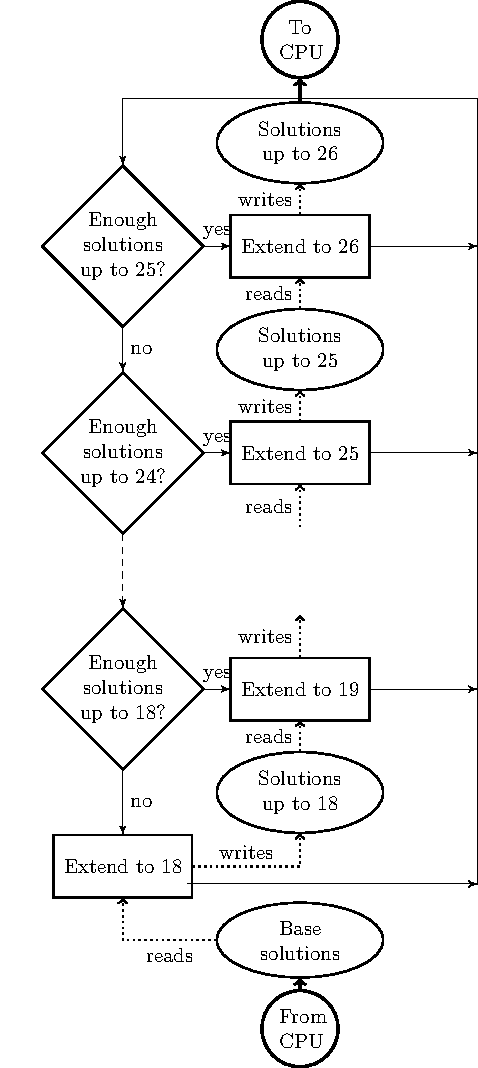
\includegraphics[scale=0.7]{figures/attack_diagram_std.pdf}
%%%%% /EPRINT %%%%
  \end{center}
%\end{minipage}
%\end{sideways}
  \caption[Simplified flow chart for the GPU part of the attack.]{Simplified flow chart for the GPU part of the attack. The start of this infinite loop is
  in the top left corner. Rectangles ``\,\protect\rectanMac\,'' represent
  snippets, ellipses ``\,\protect\elliMac\,''
  represent shared buffers, plain lines ``\,\protect\plainMac~''
  represent control flow, and dotted lines ``\,\protect\dottMac~'' represent data flow.}
  \label{fig:attack_diagram}
\end{figure}


\subsection{Implementation details}

We now give more details about the implementations of the attacks. In particular, we discuss
how partial solutions are represented at various steps in \autoref{sec:part_sol} and
we comment the code of a snippet function in \autoref{sec:snippet}. We very briefly discuss how
to tune GPU settings to use them more efficiently in \autoref{sec:gpu_tune}.

\subsubsection{Representation of partial solutions}
\label{sec:part_sol}

As the basis of our framework is to store, load and extend many partial solutions for the differential path, we need to be able to work with such objects
in an efficient way. One thus needs to define good representations for partial solutions, such that processing them is computationally simple, and managing them
in memory causes as little overhead as possible.

The representation we use is based on two types of buffers: some are holding enough information to define a \sha computation in its entirety, \ie it
contains the value of at least five (resp. sixteen) consecutive state (resp. message) words, while others only contain the necessary information to
express how the associated partial solution differs from a completely-defined one. Typically, the first kind of buffer may be used to store base solutions,
while the second is used to keep track of which neutral bits are active in a partial solution.

It is quite straightforward to define the structure of a base solution buffer, as there is little doubt about the necessary information they need
to include and the way to represent it. For instance, the 76-step base solution buffer contains the value of state words $\state_{13},\ldots,\state_{17}$
and of the message words $\expmess_6,\ldots,\expmess_{21}$. Additionally, it includes the value of $\state_{12}$; while this information is
not strictly necessary, it is useful to speed-up the computation of the activation of some neutral bits. Similar buffers without an extra state word
are used to hold partial solutions up to $\state_{36}$ and $\state_{56}$ (resp. $\state_{40}$ and $\state_{60}$ in the 80-step case). The choice
of these boundaries to define the late partial solutions were no more control is possible simply comes from the fact that a pair of messages following
the differential path of either attack is not expected to have any state differences at these steps. It is thus particularly efficient to filter
solutions that are not valid at these points.

The structures of the other buffers are also quite simple, but their instantiations may require some care to make them especially efficient.
In a nutshell, we just want such a buffer to keep a reference to a base solution and to remember the values of the currently active neutral bits.
To make this efficient and convenient to use, we would like to share a similar structure for the input and output buffers of a snippet; this would
allow to extend a partial solution that possibly already has some bits active by simply adding the newly activated bits for this step. This is the
approach we followed in our implementations, with an added refinement.

\medskip

We have already mentioned in the past section that \eg the 76-step attack contains neutral bits acting on a wide range of steps, from $\state_{18}$
to $\state_{26}$; the range for the 80-step attack is even wider, due to the use of boomerangs. Additionally, the neutral bits themselves are located on many message
words. Thus, it would seem wasteful to recompute the action of past neutral bits on message words as low as $\expmess_{14}$ while in the snippet corresponding
\eg to $\state_{24}$. Consequently, we have a strong incentive to store intermediary partial solutions in order to save some of this recomputation.

In the 76-step case, there is a natural location that may be used to define what we call \emph{extended base solutions}. As we will detail in
\autoref{sec:res_76}, neutral bits located on words $\expmess_{14}$ to $\expmess_{18}$ are only used up to $\state_{21}$, and the ones located
on words $\expmess_{19}$ to $\expmess_{21}$ are only used in later steps. Thus, it would make sense that once the active bits up to
$\expmess_{18}$ have all been determined, only the modified message words and the corresponding value for the state should be stored. There is
however no need to keep again sixteen message words in such an extended base solution, as most of them are identical to the ones of the corresponding
base solution, and as a base solution is in general extended into many distinct extended base solutions, it would not make sense to \eg add enough
message words to the latter and erase the former. One subtlety in the definition of this extended base solution is that
it also includes the message word $\expmess_{20}$. Although no neutral bits on this word
have been activated at the point where the solution is
formed, some of its bits may need to be flipped depending on the use of neutral bits on words $\expmess_{15}$ and $\expmess_{16}$, so as to
preserve message bit relations. A convenient way to remember this information is simply to preemptively add the possible contributions of the neutral
bits to $\expmess_{20}$ and to store this modified word in the extended base solution.
All in all, the buffer of extended base solution of the 76-step attack is made of twelve words: five state words $\state_{17}$ to $\state_{21}$,
six message words $\expmess_{14}$ to $\expmess_{18}$ and $\expmess_{20}$, and one word holding an identifier for the base solution from which
it is extended.

The ``inter-snippet'' buffers that refer to changes from a base or extended base solution are only made of two words consisting of concatenated
segments of the message words containing neutral bits and of a reference to the associated solution.

The 80-step attack uses similar representations but with a few variations. As we will show in \autoref{sec:res_80}, there are
more possible corrections on the messages to be performed in the 80-step attack to preserve message bit relations. Consequently, some of the precomputations of
individual neutral bit contributions are stored alongside the actual neutral bits. It is also slightly less immediate to determine where to
start defining an extended base solution, as there is no natural separation between the location of various neutral bits as there was in
the 76-step case. This is not a major issue, however, as the location of the neutral bits of a same word shared between base and extended base solutions
are not overlapping inside the word itself; splitting their representation over multiple buffers thus does not result in significant overhead.
Finally, the additional use of boomerang neutral bits, or somehow equivalently the use of more neutral bits than in the 76-step attack,
implies that the last inter-snippet buffers contain one more word  compared to the ones for early snippets and all such buffers
in the 76-step case, \ie three in total.

In \autoref{sec:res_76} and \autoref{sec:res_80}, we will describe the full content of most of the inter-snippet buffers.

\bigskip

We conclude this part by discussing some implementation aspects of the various buffers.

All of the buffers are cyclic and hold $2^{20}$ elements, regardless of their sizes, except the buffers of partial solutions extended up to
$\state_{36} \sim \state_{40}$ and $\state_{56} \sim \state_{60}$ which only have $2^{10}$ elements as they see a lower production rate due to their purely probabilistic nature.

With the exception of the buffers holding the base solutions and the collision candidates formed by partial solutions
up to $\state_{56} \sim \state_{60}$, \ie the buffers that are written or read by a CPU,
there is one instance of every buffer per block, \ie 26 buffers per GPU. This allows to use block-wise instead of global
synchronization mechanisms when updating the buffers' content,
thence reducing the overhead inherent to the use of such shared data structures.
Taken together, the buffers thus use a significant portion of the 4\,GB memory available on the \gtx, needing in the neighbourhood of 3\,GB.

We carefully took into account the presence of a limited amount of
very fast multi\-processor-specific shared memory. While the 96\,KB available per multiprocessor is
hardly enough to store the whole buffers themselves, we take advantage of it by dissociating the storage of
the buffers and of the meta-data used for their control logic, the latter being held in
shared memory. This improves the overall latency of buffer manipulations, especially in case of
heavy contention between different warps. This local shared memory is also very useful to buffer
the writes to the buffers themselves. Indeed, only a fraction of the threads of a warp often as low as $2^{-3}$
have a valid solution to write after having tested a single candidate,
and the more unsuccessful threads need to wait while the former write their solution to global memory.
It is therefore beneficial to first write the solutions to a small local warp-specific buffer and to
flush it to the main block-wise buffer as soon as it holds 32 solutions or more, thence
significantly reducing the number of accesses to the slower global memory.


\subsubsection{An example of snippet function}
\label{sec:snippet}

We now illustrate the discussion of this section by providing a commented snippet from the 76-step attack given in \autoref{lst:snippet_example} written in \textsf{CUDA C/C++}, namely a function that is taking partial solutions up to $\state_{22}$  and that is
trying to extend them up to $\state_{23}$ using neutral bits on $\expmess_{19}$. Its structure is a straightforward application of the framework, and is fairly representative of most of the
code of both of our attacks although some snippets may at first seem more complex due to their use of neutral bits located on several distinct message words.

\begin{minted}[linenos,breaklines]{c}
__device__ void stepQ23(uint32_t thread_rd_idx)
{
	uint32_t base_idx = Q22SOLBUF.get<11>(thread_rd_idx);
	uint32_t q17 = Q22SOLBUF.get<0>(thread_rd_idx);
	uint32_t q18 = Q22SOLBUF.get<1>(thread_rd_idx);
	uint32_t q19 = Q22SOLBUF.get<2>(thread_rd_idx);
	uint32_t q20 = Q22SOLBUF.get<3>(thread_rd_idx);
	uint32_t q21 = Q22SOLBUF.get<4>(thread_rd_idx);
	uint32_t m6  = BASESOLBUF.get<6>(base_idx);
	uint32_t m8  = BASESOLBUF.get<8>(base_idx);
	uint32_t m19 = BASESOLBUF.get<19>(base_idx);
	uint32_t m21 = BASESOLBUF.get<21>(base_idx);
	uint32_t m14 = Q22SOLBUF.get<5>(thread_rd_idx);
	uint32_t m22;

	uint32_t q22  = sha1_round2(q21, q20, q19, q18, q17, m21);

	uint32_t w19_q23_nb = 0;
	for (unsigned i = 0; i < 32; i++)
	{
		NEXT_NB(w19_q23_nb, W19NBQ23M);

		m19 &= ~W19NBQ23M;
		m19 |= w19_q23_nb;
		m22 = sha1_mess(m19, m14, m8, m6);

		uint32_t newq20 = q20 + w19_q23_nb;
		uint32_t newq21 = q21 + rotate_left(w19_q23_nb, 5);
		uint32_t newq22 = sha1_round2(newq21, newq20, q19, q18, q17, m21);
		uint32_t newq23 = sha1_round2(newq22, newq21, newq20, q19, q18, m22);

		uint32_t q23nessies = Qset1mask[QOFF + 23] ^ (Qprevrmask [QOFF + 23] & rotate_left(newq22, 30));
		bool valid_sol = (0 == ((newq21 ^ q21) & Qcondmask[QOFF + 21]));
		valid_sol &= (0 == ((newq22 ^ q22) & Qcondmask[QOFF + 22]));
		valid_sol &= (0 == ((newq23 ^ q23nessies) & Qcondmask[QOFF + 23]));

		uint32_t sol_val_0 = pack_update_q23_0(m19);
		uint32_t sol_val_1 = pack_update_q23_1(thread_rd_idx);

		WARP_TMP_BUF.write2(valid_sol, sol_val_0, sol_val_1, Q23SOLBUF, Q23SOLCTL);
	}
	WARP_TMP_BUF.flush2(Q23SOLBUF, Q23SOLCTL);
}
\end{minted}
\begin{figure}[tbh]
\caption{The \emph{stepQ23} function from the 76-step attack.}
\label{lst:snippet_example}
\end{figure}

\medskip

This function takes as argument a thread-dependent identifier \mintinline{c}{thread_rd_idx} for a partial solution, which is essentially an index for the buffer \mintinline{c}{Q22SOLBUF}
of solutions up to $\state_{22}$.

The partial solution is loaded from the buffer and reconstructed from lines 3 to 16. This buffer being the first one holding an extended base solution,
there is no need to reapply neutral bits and most of the work simply consists in loading the appropriate state and message words either directly from the extended base solution
buffer, or from the matching solution of the base solution buffer \mintinline{c}{BASESOLBUF}, the index of which is recovered on line 3. The only recomputation performed here
is the one of \mintinline{c}{q22} on line 16, using the \shaone round function. This would in fact not be necessary in this function, as the value could have been included in the extended base solution altogether.
This was not done because recomputing \mintinline{c}{q22} is necessary in the snippets of the following steps and causes only minimal overhead in this one, while saving a 32-bit word from the \mintinline{c}{Q22SOLBUF} buffer.

The loop from lines 18 to 41, \ie the remainder of the function, applies every combination of the five neutral bits for this step, all of which 
are located on $\expmess_{19}$. In more details, line 21 sets the register
\mintinline{c}{w19_q23_nb} to one of the 32 possible combinations. Lines 23 and 24 clear the message word \mintinline{c}{m19} of the previous neutral bit combination and applies the new one, and line 25
computes the expanded message word \mintinline{c}{m22} based on the new value for \mintinline{c}{m19}, using \shaone's message expansion. Note that this computation could actually be optimized, \eg by
precomputing the contribution of \mintinline{c}{m14}, \mintinline{c}{m8} and \mintinline{c}{m6}, which are fixed in this function.
Lines 27 to 30 compute the impact of the current neutral bit combination, first by partially recomputing the state words \mintinline{c}{newq20} and \mintinline{c}{newq21}, then fully recomputing
\mintinline{c}{newq22}, and finally computing the as yet unknown word \mintinline{c}{newq23}.
Line 32 computes a mask of sufficient conditions for the value of \mintinline{c}{newq23} based on the value of \mintinline{c}{newq22}.
Lines 33 to 35 determine if the current combination of neutral bits lead to a valid partial solution for $\state_{23}$, first by comparing the values of \mintinline{c}{q21} and  \mintinline{c}{q22}
which we know to fulfill the conditions with the updated values \mintinline{c}{newq21} and \mintinline{c}{newq22} (lines 33 and 34), and then checking \mintinline{c}{newq23} for the previously computed conditions.
Lines 37 and 38 prepare the description of the partial solution.
Finally, line 40 writes the partial solution to the buffer \mintinline{c}{Q23SOLBUF}, at the condition that it is indeed valid. As mentioned at the end of \autoref{sec:part_sol}, this is done through a warp-specific
temporary buffer, which is flushed to the actual buffer on line 42 to ensure that every valid solution is indeed eventually copied to \mintinline{c}{Q23SOLBUF}.



\subsubsection{GPU tuning}
\label{sec:gpu_tune}

After our initial implementation of the 76-step attack, we did some fine tuning of the GPU BIOS settings in order to try improving the performance.
One first objective was to ensure that the GPU fans work at 100\% during the attack, as this was strangely
not the case initially for our particular boards, and was obviously not ideal for cooling.
We also experimented with various temperature limits
that define when the GPU will start to throttle and both over-clocking and under-volting.

Taken together, these variations had a significant impact on the overall performance of the program. For a single GPU, the initial setting resulted in an estimated
time of 4.94 days to produce one 76-step freestart collision. We were able to eventually reduce this to 4.16 days. We also set-up machines with four GPUs, and observed significant
performance variations across the GPUs. This was likely due to uneven heat dissipation, as was shown by the different temperatures reached by every board. All in all, the
average expected time to obtain a collision on a single 4-GPU machine was 4.42 days per GPU, and thus about 1.1 day per machine. As the cooling was not optimal in our set-up,
reaching a performance closer to the one-GPU setting is likely to be possible.

We did not make any major changes for the 80-step attack. However, due to the higher computational cost, we only run the attack once, only using 4-GPU machines.
The collision was found after ten days, with the attack being run on sixteen 4-GPU machines.

\FloatBarrier

\subsection{Efficiency of the framework}
\label{sec:effi_fw}

We conclude this section by evaluating the performance of our framework, and in particular by assessing the relative efficiency of a GPU-based attack compared to a more traditional CPU implementation.
We provide this analysis for the 76-step attack, but the results apply entirely to the 80-step attack as well and to would-be \shaone collision attacks implemented with our framework in general.


Our GPU implementation of \shaone can compute about $2^{31.8}$ full \shaone compression functions per second on a \gtx.
Comparing this with the expected time to find a collision of 4.16 days, this means that the 76-step attack has a complexity equivalent to $2^{50.25}$ calls to the compression function for the
best-performing GPU; this increases slightly to $2^{50.34}$ when considering the 4-GPU average of 4.42 days.

Comparatively, on a Haswell Core-i5 running at 3.2\,GHz, the OpenSSL implementation of \shaone
can compute $2^{23.47}$ compression functions per second on one core. A CPU implementation of our attack
on the same processor leads to an expected time to collision of 606.12 core-days, which translates to a complexity of $2^{49.1}$
compression function calls, though this could probably be improved by vectorizing part of the CPU implementation.
This means that a single \gtx is worth 322 such CPU cores when computing the \shaone compression function, and 138 cores when
running our attack program; this increases to 146 for the best-performing GPU.
While this drop in relative efficiency was to be expected, it is somehow surprisingly small given the
complexity of our implementation and \eg the intensive use of large shared data structures. Our careful implementation thus
gives a much better value for the GPUs when compared to previous attempts at running collision attacks on such a platform:
in their work, Grechnikov and Adinetz estimated a GPU to be worth 39 CPU cores~\cite{cryptoeprint:2011:641}. This comparison should however be modulated by considering possibly uneven progress in GPUs and CPUs
since 2011 and different hardware quality. We believe that the gap between these and our results is nonetheless significant.


\section{Freestart collisions for 76-step SHA-1}
\label{sec:res_76}

This section gives the attack parameters for the 76-step freestart collision attack on \shaone.

\subsection{The differential path for most of the two first rounds}
\label{sec:app_diff_path76}

We give a graphical representation of the differential path
used in our attack up to step 36 in \autoref{fig:diff_path76}.
The meanings of the various symbols are defined
in \autoref{table:appbitconditions}.
The remainder of the path up to step 76 can easily
be determined by linerization of the step function, given the differences
in the message.

The message bit relations used in the attack for message words past $\expmess_{35}$ are given in \autoref{fig:msgbitrel76}, together with a
graphical representation in \autoref{fig:msgbitrel76_graph}.

\begin{figure}
\centering
\begin{tabular}{lcc}
$i$ & $\state_i$ & $\mess_i$\\
-4 & \nodiff\nodiff\nodiff\nodiff\nodiff\nodiff\nodiff\nodiff\nodiff\nodiff\nodiff\nodiff\nodiff\nodiff\nodiff\nodiff\nodiff\nodiff\nodiff\nodiff\nodiff\nodiff\nodiff\nodiff\nodiff\nodiff\nodiff\nodiff\nodiff\nodiff\nodiff\nodiff \\
-3 & \nodiff\nodiff\nodiff\nodiff\nodiff\nodiff\nodiff\nodiff\nodiff\nodiff\nodiff\nodiff\nodiff\nodiff\nodiff\nodiff\nodiff\nodiff\nodiff\nodiff\nodiff\nodiff\nodiff\nodiff\nodiff\nodiff\nodiff\nodiff\nodiff\nodiff\nodiff\nodiff \\
-2 & \nodiff\nodiff\nodiff\nodiff\nodiff\nodiff\nodiff\nodiff\nodiff\nodiff\nodiff\nodiff\nodiff\nodiff\nodiff\nodiff\nodiff\nodiff\nodiff\nodiff\nodiff\nodiff\nodiff\nodiff\nodiff\nodiff\nodiff\nodiff\nodiff\equaup$\monediffu$\nodiff \\
-1 & $\mnodiffz$\nodiff\nodiff\nodiff\nodiff\nodiff\nodiff\nodiff\nodiff\nodiff\nodiff\nodiff\nodiff\nodiff\nodiff\nodiff\nodiff\nodiff\nodiff\nodiff\nodiff\nodiff\nodiff\nodiff\nodiff$\mnodiffo$\nodiff\nodiff\nodiff\nodiff\nodiff$\monediffu$ \\
0 & $\mnodiffo$$\mnodiffz$\nodiff$\mnodiffz$\nodiff\nodiff\nodiff\nodiff\nodiff\nodiff\nodiff\nodiff\nodiff\nodiff\nodiff\nodiff\nodiff\nodiff\nodiff\nodiff\nodiff\nodiff\nodiff\nodiff\nodiff$\mnodiffz$\nodiff$\mnodiffz$\nodiff\nodiff\nodiff\nodiff     &  \nodiff\nodiff\nodiff\nodiff\nodiff\nodiff\nodiff\nodiff\nodiff\nodiff\nodiff\nodiff\nodiff\nodiff\nodiff\nodiff\nodiff\nodiff\nodiff\nodiff\nodiff\nodiff\nodiff\nodiff\nodiff\nodiff\nodiff$\monediffu$\nodiff\nodiff\nodiff\nodiff \\
1 & \nodiff$\mnodiffz$\nodiff$\mnodiffo$\nodiff\nodiff\nodiff\nodiff\nodiff\nodiff\nodiff\nodiff\nodiff\nodiff\nodiff\nodiff\nodiff\nodiff\nodiff\nodiff\equaup\nodiff$\mnodiffz$\nodiff\nodiff\nodiff\nodiff$\monediffu$\nodiff\nodiff\nodiff\nodiff     & \nodiff\nodiff\nodiff\nodiff\nodiff$\monediffd$\nodiff\nodiff\nodiff\nodiff\nodiff\nodiff\nodiff\nodiff\nodiff\nodiff\nodiff\nodiff\nodiff\nodiff\nodiff\nodiff\nodiff\nodiff\nodiff\nodiff\nodiff$\monediffd$$\monediffu$$\monediffu$\nodiff\nodiff \\
2 & \nodiff\nodiff\nodiff\equaup\nodiff$\monediffd$\nodiff\nodiff\nodiff\nodiff\nodiff\nodiff\nodiff\nodiff\nodiff\equaup\nodiff$\mnodiffo$\nodiff\nodiff\nodiff\nodiff$\monediffu$\nodiff\nodiff\nodiff\nodiff$\mnodiffo$\nodiff$\monediffd$\nodiff$\mnodiffo$     & $\monediffd$$\monediffu$\nodiff\nodiff$\monediffd$$\monediffu$\nodiff\nodiff\nodiff\nodiff\nodiff\nodiff\nodiff\nodiff\nodiff\nodiff\nodiff\nodiff\nodiff\nodiff\nodiff\nodiff\nodiff\nodiff\nodiff\nodiff\nodiff$\monediffu$\nodiff$\monediffd$\nodiff\nodiff \\
3 & \nodiff\nodiff\nodiff\nodiff\nodiff$\monediffd$\nodiff$\mnodiffo$\nodiff\nodiff\equaup\nodiff$\mnodiffo$\nodiff\nodiff\nodiff\nodiff$\monediffu$\nodiff\nodiff\nodiff\nodiff$\mnodiffo$\nodiff$\monediffd$\nodiff\nodiff\nodiff\equaup$\monediffd$\nodiff$\mnodiffz$     & \nodiff\nodiff\nodiff\nodiff$\monediffu$$\monediffd$\nodiff\nodiff\nodiff\nodiff\nodiff\nodiff\nodiff\nodiff\nodiff\nodiff\nodiff\nodiff\nodiff\nodiff\nodiff\nodiff\nodiff\nodiff\nodiff\nodiff\nodiff\nodiff\nodiff\nodiff$\monediffu$\nodiff \\
4 & \nodiff$\monediffd$\nodiff$\mnodiffo$\nodiff\nodiff\nodiff$\mnodiffo$$\mnodiffo$\nodiff$\mnodiffz$\nodiff$\monediffu$\nodiff\nodiff\nodiff\nodiff$\mnodiffz$$\mnodiffz$$\monediffd$$\mnodiffo$$\mnodiffo$\nodiff\nodiff$\monediffd$\nodiff\equaup\nodiff\nodiff$\mnodiffz$$\monediffu$$\mnodiffo$     & $\monediffu$$\monediffd$\nodiff\nodiff\nodiff\nodiff\nodiff\nodiff\nodiff\nodiff\nodiff\nodiff\nodiff\nodiff\nodiff\nodiff\nodiff\nodiff\nodiff\nodiff\nodiff\nodiff\nodiff\nodiff\nodiff\nodiff\nodiff$\monediffd$\nodiff\nodiff\nodiff\nodiff \\
5 & $\mnodiffo$$\monediffu$\nodiff$\mnodiffz$\nodiff\equaup\nodiff$\mnodiffz$$\mnodiffz$\equaup$\mnodiffo$$\mnodiffo$$\mnodiffo$\nodiff$\monediffd$\nodiff$\mnodiffo$$\mnodiffz$$\mnodiffo$$\monediffd$$\mnodiffz$$\mnodiffz$\nodiff$\mnodiffo$\nodiff\nodiff$\monediffu$\nodiff$\monediffu$$\mnodiffo$\nodiff$\mnodiffz$     & $\monediffu$\nodiff$\monediffu$$\monediffu$\nodiff$\monediffd$\nodiff\nodiff\nodiff\nodiff\nodiff\nodiff\nodiff\nodiff\nodiff\nodiff\nodiff\nodiff\nodiff\nodiff\nodiff\nodiff\nodiff\nodiff\nodiff\nodiff\nodiff$\monediffd$$\monediffu$$\monediffd$\nodiff\nodiff \\
6 & $\mnodiffz$$\mnodiffz$\nodiff$\monediffd$\equaup$\monediffd$$\mnodiffo$$\monediffd$$\mnodiffo$$\monediffd$$\monediffd$$\monediffu$$\monediffu$$\monediffu$$\monediffu$\equaup$\mnodiffz$$\mnodiffo$$\monediffu$$\mnodiffz$$\monediffd$\nodiff$\monediffd$$\monediffd$\nodiff$\mnodiffo$$\mnodiffo$\nodiff$\mnodiffo$\nodiff$\mnodiffz$$\monediffd$     & \nodiff\nodiff$\monediffu$$\monediffd$$\monediffu$$\monediffu$\nodiff\nodiff\nodiff\nodiff\nodiff\nodiff\nodiff\nodiff\nodiff\nodiff\nodiff\nodiff\nodiff\nodiff\nodiff\nodiff\nodiff\nodiff\nodiff\nodiff\nodiff\nodiff\nodiff$\monediffu$\nodiff\nodiff \\
7 & $\mnodiffo$$\monediffu$\nodiff$\monediffd$\equaup$\monediffu$$\monediffd$$\mnodiffz$$\monediffd$$\monediffu$$\mnodiffo$$\mnodiffz$$\monediffu$$\monediffd$$\mnodiffz$\equaup$\monediffu$$\monediffu$$\monediffd$$\monediffu$$\mnodiffo$\equaup$\mnodiffo$\nodiff$\mnodiffz$$\monediffu$\nodiff\nodiff$\mnodiffz$\nodiff$\mnodiffo$$\mnodiffo$     & $\monediffu$\nodiff$\monediffu$$\monediffd$$\monediffd$$\monediffd$\nodiff\nodiff\nodiff\nodiff\nodiff\nodiff\nodiff\nodiff\nodiff\nodiff\nodiff\nodiff\nodiff\nodiff\nodiff\nodiff\nodiff\nodiff\nodiff\nodiff\nodiff$\monediffu$$\monediffd$\nodiff$\monediffd$\nodiff \\
8 & $\monediffu$$\monediffd$\nodiff$\mnodiffo$\nodiff\nodiff$\monediffu$$\monediffd$$\monediffd$$\monediffd$$\monediffd$$\monediffd$$\monediffd$$\monediffd$$\monediffd$$\monediffd$$\monediffd$$\monediffd$$\monediffd$$\monediffd$$\mnodiffo$$\monediffd$$\monediffu$$\monediffu$$\mnodiffo$$\mnodiffo$\nodiff$\monediffd$\nodiff\nodiff$\monediffu$$\mnodiffz$     & \nodiff\nodiff$\monediffd$\nodiff\nodiff\nodiff\nodiff\nodiff\nodiff\nodiff\nodiff\nodiff\nodiff\nodiff\nodiff\nodiff\nodiff\nodiff\nodiff\nodiff\nodiff\nodiff\nodiff\nodiff\nodiff\nodiff\nodiff$\monediffd$\nodiff\nodiff\nodiff\nodiff \\
9 & $\monediffd$$\monediffd$$\monediffu$$\mnodiffz$\nodiff$\mnodiffo$\nodiff$\mnodiffz$$\mnodiffo$$\mnodiffz$\nodiff$\mnodiffo$$\mnodiffz$$\mnodiffz$$\mnodiffz$\nodiff$\mnodiffo$$\mnodiffz$$\monediffu$$\monediffd$\nodiff$\mnodiffz$\nodiff$\mnodiffo$$\mnodiffz$$\mnodiffz$$\monediffd$$\mnodiffo$\nodiff$\mnodiffo$$\mnodiffz$\nodiff     & \nodiff\nodiff$\monediffu$\nodiff\nodiff$\monediffu$\nodiff\nodiff\nodiff\nodiff\nodiff\nodiff\nodiff\nodiff\nodiff\nodiff\nodiff\nodiff\nodiff\nodiff\nodiff\nodiff\nodiff\nodiff\nodiff\nodiff\nodiff$\monediffd$$\monediffu$$\monediffu$\nodiff\nodiff \\
10 & $\monediffd$$\mnodiffo$$\mnodiffz$\nodiff$\mnodiffo$\nodiff\nodiff\nodiff$\mnodiffo$$\mnodiffz$$\mnodiffz$$\mnodiffz$$\mnodiffo$$\mnodiffo$$\mnodiffo$$\mnodiffz$$\mnodiffo$$\mnodiffo$$\mnodiffz$$\mnodiffz$$\mnodiffo$\nodiff\nodiff$\mnodiffo$$\mnodiffo$$\mnodiffo$\nodiff\nodiff$\mnodiffo$$\mnodiffz$\nodiff\nodiff     & $\monediffd$$\monediffd$$\monediffu$\nodiff$\monediffu$$\monediffd$\nodiff\nodiff\nodiff\nodiff\nodiff\nodiff\nodiff\nodiff\nodiff\nodiff\nodiff\nodiff\nodiff\nodiff\nodiff\nodiff\nodiff\nodiff\nodiff\nodiff\nodiff$\monediffd$\nodiff$\monediffu$\nodiff\nodiff \\
11 & $\mnodiffo$\nodiff\nodiff$\monediffd$$\mnodiffo$\nodiff\nodiff\nodiff\nodiff\nodiff\nodiff\nodiff\nodiff\nodiff\nodiff\nodiff\nodiff\nodiff\nodiff\nodiff$\mnodiffo$$\mnodiffz$\nodiff\nodiff\nodiff\nodiff\nodiff\nodiff$\mnodiffo$\nodiff\equaup\nodiff     & \nodiff\nodiff\nodiff\nodiff$\monediffd$$\monediffu$\nodiff\nodiff\nodiff\nodiff\nodiff\nodiff\nodiff\nodiff\nodiff\nodiff\nodiff\nodiff\nodiff\nodiff\nodiff\nodiff\nodiff\nodiff\nodiff\nodiff\nodiff\nodiff\nodiff\nodiff$\monediffd$\nodiff \\
12 & $\monediffu$\nodiff$\monediffu$\nodiff\nodiff$\mnodiffo$\nodiff\nodiff\nodiff\nodiff\nodiff\nodiff\nodiff\nodiff\nodiff\nodiff\nodiff\nodiff\nodiff\nodiff\nodiff\nodiff\nodiff\nodiff\equaup\nodiff\nodiff\nodiff\nodiff\nodiff\nodiff\nodiff     & $\monediffd$$\monediffu$\nodiff\nodiff\nodiff\nodiff\nodiff\nodiff\nodiff\nodiff\nodiff\nodiff\nodiff\nodiff\nodiff\nodiff\nodiff\nodiff\nodiff\nodiff\nodiff\nodiff\nodiff\nodiff\nodiff\nodiff\nodiff$\monediffu$\nodiff\nodiff\nodiff\nodiff \\
13 & $\mnodiffz$\nodiff$\monediffu$\nodiff$\mnodiffo$$\mnodiffz$\nodiff\nodiff\nodiff\nodiff\nodiff\nodiff\nodiff\nodiff\nodiff\nodiff\nodiff\nodiff\nodiff\nodiff\nodiff\nodiff\nodiff\nodiff\nodiff\nodiff$\monediffd$\nodiff\nodiff\nodiff\nodiff$\mnodiffz$     & $\monediffu$\nodiff$\monediffd$$\monediffd$\nodiff$\monediffd$\nodiff\nodiff\nodiff\nodiff\nodiff\nodiff\nodiff\nodiff\nodiff\nodiff\nodiff\nodiff\nodiff\nodiff\nodiff\nodiff\nodiff\nodiff\nodiff\nodiff\nodiff$\monediffu$$\monediffd$$\monediffd$\nodiff\nodiff \\
14 & \nodiff\nodiff$\monediffu$\nodiff\nodiff\nodiff\nodiff\nodiff\nodiff\nodiff\nodiff\nodiff\nodiff\nodiff\nodiff\nodiff\nodiff\nodiff\nodiff\nodiff\nodiff\nodiff\nodiff\nodiff\nodiff\nodiff\nodiff\nodiff$\mnodiffz$\nodiff\nodiff$\mnodiffo$     & \nodiff\nodiff$\monediffd$\nodiff$\monediffd$$\monediffu$\nodiff\nodiff\nodiff\nodiff\nodiff\nodiff\nodiff\nodiff\nodiff\nodiff\nodiff\nodiff\nodiff\nodiff\nodiff\nodiff\nodiff\nodiff\nodiff\nodiff\nodiff\nodiff\nodiff$\monediffd$\nodiff\nodiff \\
15 & $\mnodiffo$$\monediffd$\nodiff\nodiff\nodiff\nodiff\nodiff\nodiff\nodiff\nodiff\nodiff\nodiff\nodiff\nodiff\nodiff\nodiff\nodiff\nodiff\nodiff\nodiff\nodiff\nodiff\nodiff\nodiff\nodiff\nodiff\nodiff\nodiff$\mnodiffo$\nodiff\diffup\nodiff     & $\monediffu$\nodiff$\monediffd$$\monediffu$$\monediffu$$\monediffu$\nodiff\nodiff\nodiff\nodiff\nodiff\nodiff\nodiff\nodiff\nodiff\nodiff\nodiff\nodiff\nodiff\nodiff\nodiff\nodiff\nodiff\nodiff\nodiff\nodiff\nodiff$\monediffu$$\monediffd$\nodiff\nodiff\nodiff \\
16 & $\monediffu$\nodiff\nodiff$\mnodiffo$$\mnodiffz$\nodiff\nodiff\nodiff\nodiff\nodiff\nodiff\nodiff\nodiff\nodiff\nodiff\nodiff\nodiff\nodiff\nodiff\nodiff\nodiff\nodiff\nodiff\nodiff\nodiff\nodiff\nodiff\nodiff\nodiff\nodiff\equaup\nodiff     & $\monediffd$\nodiff$\monediffd$$\monediffu$\nodiff\nodiff\nodiff\nodiff\nodiff\nodiff\nodiff\nodiff\nodiff\nodiff\nodiff\nodiff\nodiff\nodiff\nodiff\nodiff\nodiff\nodiff\nodiff\nodiff\nodiff\nodiff\nodiff$\monediffd$\nodiff\nodiff\nodiff\nodiff \\
17 & $\monediffu$\nodiff$\monediffd$$\mnodiffo$\nodiff\nodiff\nodiff\nodiff\nodiff\nodiff\nodiff\nodiff\nodiff\nodiff\nodiff\nodiff\nodiff\nodiff\nodiff\nodiff\nodiff\nodiff\nodiff\nodiff\nodiff\nodiff\nodiff\nodiff\nodiff\nodiff\diffup\nodiff     & \nodiff\nodiff\nodiff\nodiff\nodiff\nodiff\nodiff\nodiff\nodiff\nodiff\nodiff\nodiff\nodiff\nodiff\nodiff\nodiff\nodiff\nodiff\nodiff\nodiff\nodiff\nodiff\nodiff\nodiff\nodiff\nodiff\nodiff\nodiff$\monediffd$$\monediffu$\nodiff\nodiff \\
18 & $\monediffu$\nodiff\nodiff\nodiff$\mnodiffo$\nodiff\nodiff\nodiff\nodiff\nodiff\nodiff\nodiff\nodiff\nodiff\nodiff\nodiff\nodiff\nodiff\nodiff\nodiff\nodiff\nodiff\nodiff\nodiff\nodiff\nodiff\nodiff\nodiff\nodiff\nodiff\nodiff\equaup     & $\monediffu$\nodiff$\monediffu$$\monediffd$$\monediffu$\nodiff\nodiff\nodiff\nodiff\nodiff\nodiff\nodiff\nodiff\nodiff\nodiff\nodiff\nodiff\nodiff\nodiff\nodiff\nodiff\nodiff\nodiff\nodiff\nodiff\nodiff\nodiff$\monediffd$\nodiff\nodiff\nodiff\nodiff \\
19 & \nodiff$\monediffd$\nodiff\nodiff\diffrightup\nodiff\nodiff\nodiff\nodiff\nodiff\nodiff\nodiff\nodiff\nodiff\nodiff\nodiff\nodiff\nodiff\nodiff\nodiff\nodiff\nodiff\nodiff\nodiff\nodiff\nodiff\nodiff\nodiff\nodiff\nodiff\nodiff\nodiff     & \nodiff\nodiff\nodiff\nodiff$\monediffd$\nodiff\nodiff\nodiff\nodiff\nodiff\nodiff\nodiff\nodiff\nodiff\nodiff\nodiff\nodiff\nodiff\nodiff\nodiff\nodiff\nodiff\nodiff\nodiff\nodiff\nodiff\nodiff$\monediffu$$\monediffd$\nodiff\nodiff\nodiff \\
20 & $\monediffd$\nodiff\diffrightup\diffrightupup\nodiff\nodiff\nodiff\nodiff\nodiff\nodiff\nodiff\nodiff\nodiff\nodiff\nodiff\nodiff\nodiff\nodiff\nodiff\nodiff\nodiff\nodiff\nodiff\nodiff\nodiff\nodiff\nodiff\nodiff\nodiff\nodiff\nodiff\nodiff     & \nodiff$\monediffu$$\monediffu$$\monediffu$$\monediffu$\nodiff\nodiff\nodiff\nodiff\nodiff\nodiff\nodiff\nodiff\nodiff\nodiff\nodiff\nodiff\nodiff\nodiff\nodiff\nodiff\nodiff\nodiff\nodiff\nodiff\nodiff\nodiff$\monediffu$\nodiff\nodiff\nodiff\nodiff \\
21 & $\monediffd$\nodiff$\monediffd$\diffrightup\nodiff\nodiff\nodiff\nodiff\nodiff\nodiff\nodiff\nodiff\nodiff\nodiff\nodiff\nodiff\nodiff\nodiff\nodiff\nodiff\nodiff\nodiff\nodiff\nodiff\nodiff\nodiff\nodiff\nodiff\nodiff\nodiff\nodiff\nodiff     & \nodiff\nodiff\nodiff\nodiff$\monediffd$\nodiff\nodiff\nodiff\nodiff\nodiff\nodiff\nodiff\nodiff\nodiff\nodiff\nodiff\nodiff\nodiff\nodiff\nodiff\nodiff\nodiff\nodiff\nodiff\nodiff\nodiff\nodiff$\monediffu$\nodiff$\monediffu$\nodiff\nodiff \\
22 & $\monediffd$\nodiff\nodiff\nodiff\equarightupup\nodiff\nodiff\nodiff\nodiff\nodiff\nodiff\nodiff\nodiff\nodiff\nodiff\nodiff\nodiff\nodiff\nodiff\nodiff\nodiff\nodiff\nodiff\nodiff\nodiff\nodiff\nodiff\nodiff\nodiff\nodiff\nodiff\nodiff     & \nodiff$\monediffd$$\monediffu$$\monediffu$\nodiff\nodiff\nodiff\nodiff\nodiff\nodiff\nodiff\nodiff\nodiff\nodiff\nodiff\nodiff\nodiff\nodiff\nodiff\nodiff\nodiff\nodiff\nodiff\nodiff\nodiff\nodiff\nodiff$\monediffu$\nodiff\nodiff\nodiff\nodiff \\
23 & $\monediffd$\nodiff$\monediffu$\nodiff\equarightup\nodiff\nodiff\nodiff\nodiff\nodiff\nodiff\nodiff\nodiff\nodiff\nodiff\nodiff\nodiff\nodiff\nodiff\nodiff\nodiff\nodiff\nodiff\nodiff\nodiff\nodiff\nodiff\nodiff\nodiff\nodiff\nodiff\nodiff     & $\monediffd$\nodiff$\monediffu$$\monediffd$$\monediffu$\nodiff\nodiff\nodiff\nodiff\nodiff\nodiff\nodiff\nodiff\nodiff\nodiff\nodiff\nodiff\nodiff\nodiff\nodiff\nodiff\nodiff\nodiff\nodiff\nodiff\nodiff\nodiff$\monediffu$$\monediffd$$\monediffu$\nodiff\nodiff \\
24 & \nodiff\nodiff\nodiff\nodiff\diffrightupup\nodiff\nodiff\nodiff\nodiff\nodiff\nodiff\nodiff\nodiff\nodiff\nodiff\nodiff\nodiff\nodiff\nodiff\nodiff\nodiff\nodiff\nodiff\nodiff\nodiff\nodiff\nodiff\nodiff\nodiff\nodiff\nodiff\nodiff     & $\monediffd$$\monediffd$$\monediffu$\nodiff$\monediffu$\nodiff\nodiff\nodiff\nodiff\nodiff\nodiff\nodiff\nodiff\nodiff\nodiff\nodiff\nodiff\nodiff\nodiff\nodiff\nodiff\nodiff\nodiff\nodiff\nodiff\nodiff\nodiff\nodiff\nodiff\nodiff\nodiff\nodiff \\
25 & \nodiff\nodiff$\monediffd$\nodiff\diffrightup\nodiff\nodiff\nodiff\nodiff\nodiff\nodiff\nodiff\nodiff\nodiff\nodiff\nodiff\nodiff\nodiff\nodiff\nodiff\nodiff\nodiff\nodiff\nodiff\nodiff\nodiff\nodiff\nodiff\nodiff\nodiff\nodiff\nodiff     & $\monediffd$\nodiff$\monediffu$$\monediffu$\nodiff\nodiff\nodiff\nodiff\nodiff\nodiff\nodiff\nodiff\nodiff\nodiff\nodiff\nodiff\nodiff\nodiff\nodiff\nodiff\nodiff\nodiff\nodiff\nodiff\nodiff\nodiff\nodiff\nodiff\nodiff$\monediffu$\nodiff\nodiff \\
26 & $\monediffd$\nodiff\nodiff\nodiff\diffrightupup\nodiff\nodiff\nodiff\nodiff\nodiff\nodiff\nodiff\nodiff\nodiff\nodiff\nodiff\nodiff\nodiff\nodiff\nodiff\nodiff\nodiff\nodiff\nodiff\nodiff\nodiff\nodiff\nodiff\nodiff\nodiff\nodiff\equaup     & \nodiff$\monediffd$\nodiff$\monediffu$$\monediffd$\nodiff\nodiff\nodiff\nodiff\nodiff\nodiff\nodiff\nodiff\nodiff\nodiff\nodiff\nodiff\nodiff\nodiff\nodiff\nodiff\nodiff\nodiff\nodiff\nodiff\nodiff\nodiff$\monediffu$\nodiff\nodiff\nodiff\nodiff \\
27 & \nodiff$\monediffd$$\monediffd$\nodiff\equarightup\nodiff\nodiff\nodiff\nodiff\nodiff\nodiff\nodiff\nodiff\nodiff\nodiff\nodiff\nodiff\nodiff\nodiff\nodiff\nodiff\nodiff\nodiff\nodiff\nodiff\nodiff\nodiff\nodiff\nodiff\nodiff\nodiff\nodiff     & $\monediffu$\nodiff$\monediffu$$\monediffd$\nodiff\nodiff\nodiff\nodiff\nodiff\nodiff\nodiff\nodiff\nodiff\nodiff\nodiff\nodiff\nodiff\nodiff\nodiff\nodiff\nodiff\nodiff\nodiff\nodiff\nodiff\nodiff\nodiff\nodiff$\monediffu$$\monediffu$\nodiff\nodiff \\
28 & \nodiff\nodiff\equarightup\diffrightupup\diffrightupup\nodiff\nodiff\nodiff\nodiff\nodiff\nodiff\nodiff\nodiff\nodiff\nodiff\nodiff\nodiff\nodiff\nodiff\nodiff\nodiff\nodiff\nodiff\nodiff\nodiff\nodiff\nodiff\nodiff\nodiff\nodiff\nodiff\nodiff     & \nodiff$\monediffu$\nodiff\nodiff$\monediffu$\nodiff\nodiff\nodiff\nodiff\nodiff\nodiff\nodiff\nodiff\nodiff\nodiff\nodiff\nodiff\nodiff\nodiff\nodiff\nodiff\nodiff\nodiff\nodiff\nodiff\nodiff\nodiff\nodiff\nodiff\nodiff\nodiff\nodiff \\
29 & \nodiff\nodiff\nodiff\equarightup\equarightup\nodiff\nodiff\nodiff\nodiff\nodiff\nodiff\nodiff\nodiff\nodiff\nodiff\nodiff\nodiff\nodiff\nodiff\nodiff\nodiff\nodiff\nodiff\nodiff\nodiff\nodiff\nodiff\nodiff\nodiff\nodiff\nodiff\nodiff    & $\monediffu$\nodiff$\monediffu$$\monediffd$\nodiff\nodiff\nodiff\nodiff\nodiff\nodiff\nodiff\nodiff\nodiff\nodiff\nodiff\nodiff\nodiff\nodiff\nodiff\nodiff\nodiff\nodiff\nodiff\nodiff\nodiff\nodiff\nodiff\nodiff\nodiff\nodiff\nodiff\nodiff \\
30 & $\monediffd$\nodiff\nodiff\nodiff\nodiff\nodiff\nodiff\nodiff\nodiff\nodiff\nodiff\nodiff\nodiff\nodiff\nodiff\nodiff\nodiff\nodiff\nodiff\nodiff\nodiff\nodiff\nodiff\nodiff\nodiff\nodiff\nodiff\nodiff\nodiff\nodiff\nodiff\nodiff     & $\monediffd$\nodiff$\monediffu$$\monediffu$$\monediffu$\nodiff\nodiff\nodiff\nodiff\nodiff\nodiff\nodiff\nodiff\nodiff\nodiff\nodiff\nodiff\nodiff\nodiff\nodiff\nodiff\nodiff\nodiff\nodiff\nodiff\nodiff\nodiff$\monediffu$\nodiff\nodiff\nodiff\nodiff \\
31 & $\monediffd$\nodiff\equarightupup\nodiff\nodiff\nodiff\nodiff\nodiff\nodiff\nodiff\nodiff\nodiff\nodiff\nodiff\nodiff\nodiff\nodiff\nodiff\nodiff\nodiff\nodiff\nodiff\nodiff\nodiff\nodiff\nodiff\nodiff\nodiff\nodiff\nodiff\nodiff\nodiff     & $\monediffd$\nodiff\nodiff$\monediffu$$\monediffu$\nodiff\nodiff\nodiff\nodiff\nodiff\nodiff\nodiff\nodiff\nodiff\nodiff\nodiff\nodiff\nodiff\nodiff\nodiff\nodiff\nodiff\nodiff\nodiff\nodiff\nodiff\nodiff$\monediffu$\nodiff\nodiff\nodiff\nodiff \\
32 & \nodiff\nodiff\nodiff\nodiff\nodiff\nodiff\nodiff\nodiff\nodiff\nodiff\nodiff\nodiff\nodiff\nodiff\nodiff\nodiff\nodiff\nodiff\nodiff\nodiff\nodiff\nodiff\nodiff\nodiff\nodiff\nodiff\nodiff\nodiff\nodiff\nodiff\nodiff\nodiff     & $\monediffd$\nodiff$\monediffu$\nodiff\nodiff\nodiff\nodiff\nodiff\nodiff\nodiff\nodiff\nodiff\nodiff\nodiff\nodiff\nodiff\nodiff\nodiff\nodiff\nodiff\nodiff\nodiff\nodiff\nodiff\nodiff\nodiff\nodiff\nodiff\nodiff\nodiff\nodiff\nodiff \\
33 & \nodiff\nodiff\diffrightup\nodiff\nodiff\nodiff\nodiff\nodiff\nodiff\nodiff\nodiff\nodiff\nodiff\nodiff\nodiff\nodiff\nodiff\nodiff\nodiff\nodiff\nodiff\nodiff\nodiff\nodiff\nodiff\nodiff\nodiff\nodiff\nodiff\nodiff\nodiff\nodiff     & \nodiff\nodiff\nodiff\nodiff\nodiff\nodiff\nodiff\nodiff\nodiff\nodiff\nodiff\nodiff\nodiff\nodiff\nodiff\nodiff\nodiff\nodiff\nodiff\nodiff\nodiff\nodiff\nodiff\nodiff\nodiff\nodiff\nodiff\nodiff\nodiff\nodiff\nodiff\nodiff \\
34 & \nodiff\nodiff\nodiff\nodiff\nodiff\nodiff\nodiff\nodiff\nodiff\nodiff\nodiff\nodiff\nodiff\nodiff\nodiff\nodiff\nodiff\nodiff\nodiff\nodiff\nodiff\nodiff\nodiff\nodiff\nodiff\nodiff\nodiff\nodiff\nodiff\nodiff\nodiff\nodiff     & \nodiff\nodiff\nodiff\nodiff\nodiff\nodiff\nodiff\nodiff\nodiff\nodiff\nodiff\nodiff\nodiff\nodiff\nodiff\nodiff\nodiff\nodiff\nodiff\nodiff\nodiff\nodiff\nodiff\nodiff\nodiff\nodiff\nodiff\nodiff\nodiff\nodiff\nodiff\nodiff \\
35 & \nodiff\nodiff\nodiff\nodiff\nodiff\nodiff\nodiff\nodiff\nodiff\nodiff\nodiff\nodiff\nodiff\nodiff\nodiff\nodiff\nodiff\nodiff\nodiff\nodiff\nodiff\nodiff\nodiff\nodiff\nodiff\nodiff\nodiff\nodiff\nodiff\nodiff\nodiff\nodiff     & \nodiff\nodiff$\monediffu$\nodiff\nodiff\nodiff\nodiff\nodiff\nodiff\nodiff\nodiff\nodiff\nodiff\nodiff\nodiff\nodiff\nodiff\nodiff\nodiff\nodiff\nodiff\nodiff\nodiff\nodiff\nodiff\nodiff\nodiff\nodiff\nodiff\nodiff\nodiff\nodiff \\
36 & \nodiff\nodiff\nodiff\nodiff\nodiff\nodiff\nodiff\nodiff\nodiff\nodiff\nodiff\nodiff\nodiff\nodiff\nodiff\nodiff\nodiff\nodiff\nodiff\nodiff\nodiff\nodiff\nodiff\nodiff\nodiff\nodiff\nodiff\nodiff\nodiff\nodiff\nodiff\nodiff \\
\end{tabular}
\caption{The differential path of the 76-step attack up to step 36.\label{fig:diff_path76}}
\end{figure}

\begingroup
\fontsize{8pt}{9pt}\selectfont
\begin{verbbox}
- W54[29] ^ W55[29] = 0
- W53[29] ^ W55[29] = 0
- W51[4] ^ W55[29] = 0
- W49[29] ^ W50[29] = 0
- W48[29] ^ W50[29] = 0
- W47[28] ^ W47[29] = 1
- W46[4] ^ W50[29] = 0
- W46[28] ^ W47[28] = 0
- W46[29] ^ W47[28] = 1
- W45[28] ^ W47[28] = 0
- W44[29] ^ W44[30] = 0
- W43[3] ^ W47[28] = 0
- W43[4] ^ W47[28] = 1
- W42[29] ^ W47[28] = 1
- W41[4] ^ W47[28] = 0
- W40[29] ^ W47[28] = 0
- W39[4] ^ W47[28] = 1
- W37[4] ^ W47[28] = 0
- W59[4] ^ W63[29] = 0
- W57[4] ^ W59[29] = 0
- W74[0] = 1
- W75[5] = 0
- W73[1] ^ W74[6] = 1
- W71[5] ^ W75[30] = 0
- W70[0] ^ W75[30] = 1
\end{verbbox}
\endgroup
\begin{figure}
\begin{center}
\begin{tabular}{l l l}
 $\expmess_{54}[29] \oplus \expmess_{55}[29] = 0$ & $\expmess_{53}[29] \oplus \expmess_{55}[29] = 0$ & $\expmess_{51}[4]  \oplus \expmess_{55}[29] = 0$\\
 $\expmess_{49}[29] \oplus \expmess_{50}[29] = 0$ & $\expmess_{48}[29] \oplus \expmess_{50}[29] = 0$ & $\expmess_{47}[28] \oplus \expmess_{47}[29] = 1$\\
 $\expmess_{46}[4]  \oplus \expmess_{50}[29] = 0$ & $\expmess_{46}[28] \oplus \expmess_{47}[28] = 0$ & $\expmess_{46}[29] \oplus \expmess_{47}[28] = 1$\\
 $\expmess_{45}[28] \oplus \expmess_{47}[28] = 0$ & $\expmess_{44}[29] \oplus \expmess_{44}[30] = 0$ & $\expmess_{43}[3]  \oplus \expmess_{47}[28] = 0$\\
 $\expmess_{43}[4]  \oplus \expmess_{47}[28] = 1$ & $\expmess_{42}[29] \oplus \expmess_{47}[28] = 1$ & $\expmess_{41}[4]  \oplus \expmess_{47}[28] = 0$\\
 $\expmess_{40}[29] \oplus \expmess_{47}[28] = 0$ & $\expmess_{39}[4]  \oplus \expmess_{47}[28] = 1$ & $\expmess_{37}[4]  \oplus \expmess_{47}[28] = 0$\\
 $\expmess_{59}[4]  \oplus \expmess_{63}[29] = 0$ & $\expmess_{57}[4]  \oplus \expmess_{59}[29] = 0$ & $\expmess_{74}[0] = 1$\\ 
 $\expmess_{75}[5] = 0$ & $\expmess_{73}[1]  \oplus \expmess_{74}[6] = 1$ & $\expmess_{71}[5]  \oplus \expmess_{75}[30] = 0$\\
 $\expmess_{70}[0]  \oplus \expmess_{75}[30] = 1$\\
\end{tabular}
\end{center}
  \caption{The message bit relations of the 76-step attack for message words $\expmess_{36}$ to $\expmess_{75}$.
  \label{fig:msgbitrel76}}
\end{figure}

\begingroup
\fontsize{8pt}{9pt}\selectfont
\begin{verbbox}
W36:	 . . . . . . . . . . . . . . . . . . . . . . . . . . . . . . . .
W37:	 . . . . . . . . . . . . . . . . . . . . . . . . . . . a . . . .
W38:	 . . . . . . . . . . . . . . . . . . . . . . . . . . . . . . . .
W39:	 . . . . . . . . . . . . . . . . . . . . . . . . . . . A . . . .
W40:	 . . a . . . . . . . . . . . . . . . . . . . . . . . . . . . . .
W41:	 . . . . . . . . . . . . . . . . . . . . . . . . . . . a . . . .
W42:	 . . A . . . . . . . . . . . . . . . . . . . . . . . . . . . . .
W43:	 . . . . . . . . . . . . . . . . . . . . . . . . . . . A a . . .
W44:	 . b b . . . . . . . . . . . . . . . . . . . . . . . . . . . . .
W45:	 . . . a . . . . . . . . . . . . . . . . . . . . . . . . . . . .
W46:	 . . A a . . . . . . . . . . . . . . . . . . . . . . . c . . . .
W47:	 . . A a . . . . . . . . . . . . . . . . . . . . . . . . . . . .
W48:	 . . c . . . . . . . . . . . . . . . . . . . . . . . . . . . . .
W49:	 . . c . . . . . . . . . . . . . . . . . . . . . . . . . . . . .
W50:	 . . c . . . . . . . . . . . . . . . . . . . . . . . . . . . . .
W51:	 . . . . . . . . . . . . . . . . . . . . . . . . . . . d . . . .
W52:	 . . . . . . . . . . . . . . . . . . . . . . . . . . . . . . . .
W53:	 . . d . . . . . . . . . . . . . . . . . . . . . . . . . . . . .
W54:	 . . d . . . . . . . . . . . . . . . . . . . . . . . . . . . . .
W55:	 . . d . . . . . . . . . . . . . . . . . . . . . . . . . . . . .
W56:	 . . . . . . . . . . . . . . . . . . . . . . . . . . . . . . . .
W57:	 . . . . . . . . . . . . . . . . . . . . . . . . . . . e . . . .
W58:	 . . . . . . . . . . . . . . . . . . . . . . . . . . . . . . . .
W59:	 . . e . . . . . . . . . . . . . . . . . . . . . . . . f . . . .
W60:	 . . . . . . . . . . . . . . . . . . . . . . . . . . . . . . . .
W61:	 . . . . . . . . . . . . . . . . . . . . . . . . . . . . . . . .
W62:	 . . . . . . . . . . . . . . . . . . . . . . . . . . . . . . . .
W63:	 . . f . . . . . . . . . . . . . . . . . . . . . . . . . . . . .
W64:	 . . . . . . . . . . . . . . . . . . . . . . . . . . . . . . . .
W65:	 . . . . . . . . . . . . . . . . . . . . . . . . . . . . . . . .
W66:	 . . . . . . . . . . . . . . . . . . . . . . . . . . . . . . . .
W67:	 . . . . . . . . . . . . . . . . . . . . . . . . . . . . . . . .
W68:	 . . . . . . . . . . . . . . . . . . . . . . . . . . . . . . . .
W69:	 . . . . . . . . . . . . . . . . . . . . . . . . . . . . . . . .
W70:	 . . . . . . . . . . . . . . . . . . . . . . . . . . . . . . . g
W71:	 . . . . . . . . . . . . . . . . . . . . . . . . . . G . . . . .
W72:	 . . . . . . . . . . . . . . . . . . . . . . . . . . . . . . . .
W73:	 . . . . . . . . . . . . . . . . . . . . . . . . . . . . . . h .
W74:	 . . . . . . . . . . . . . . . . . . . . . . . . . H . . . . . 1
W75:	 . G . . . . . . . . . . . . . . . . . . . . . . . . 0 . . . . .
\end{verbbox}
\endgroup

\begin{figure}[ht]
\centering
  \theverbbox
  \caption{The message bit-relations used in the attack for words $\expmess_{36}$ to $\expmess_{75}$ (graphical representation).
  A dot (``\texttt{.}'') means an absence of condition. A zero (``\texttt{0}'') or one (``\texttt{1}'') character represents a bit unconditionally set to 0 or 1.
  A pair of two identical letters $x$ means that the two bits have the same value. A pair of two
  letters $x$ and $X$ means that the two bits have different values.
  \label{fig:msgbitrel76_graph}}
\end{figure}

\subsection{The neutral bits}
\label{sec:neutral_bits76}
We give here the list of the neutral bits used in the attack.
There are fifty-one of them over the eight message words
$\expmess_{14}$ to $\expmess_{21}$, distributed as
follows:
\begin{itemize}
\item $\expmess_{14}$: 9 neutral bits at  bit positions (starting with the least significant bit (\emph{LSB}) at zero) 5,6,7,8,9,10,11,12,13
\item $\expmess_{15}$: 11 neutral bits at positions 5,6,7,8,9,10,11,12,13,14,16
\item $\expmess_{16}$: 8 neutral bits at positions 6,7,8,9,10,11,13,16
\item $\expmess_{17}$: 5 neutral bits at positions 10,11,12,13,19
\item $\expmess_{18}$: 2 neutral bits at positions 15,16
\item $\expmess_{19}$: 8 neutral bits at positions 6,7,8,9,10,11,12,14
\item $\expmess_{20}$: 5 neutral bits at positions 0,6,11,12,13
\item $\expmess_{21}$: 3 neutral bits at positions 11,16,17
\end{itemize}
We give a graphical representation of the repartition of these neutral bits in \autoref{fig:neutbits76}.

\begin{figure}
\centering
\begin{tabular}{l c}
$\expmess_{14}$: & \nodiff\nodiff\nodiff\nodiff\nodiff\nodiff\nodiff\nodiff\nodiff\nodiff\nodiff\nodiff\nodiff\nodiff\nodiff\nodiff\nodiff\nodiff\onediff\onediff\onediff\onediff\onediff\onediff\onediff\onediff\onediff\nodiff\nodiff\nodiff\nodiff\nodiff \\
$\expmess_{15}$: & \nodiff\nodiff\nodiff\nodiff\nodiff\nodiff\nodiff\nodiff\nodiff\nodiff\nodiff\nodiff\nodiff\nodiff\nodiff\onediff\nodiff\onediff\onediff\onediff\onediff\onediff\onediff\onediff\onediff\onediff\onediff\nodiff\nodiff\nodiff\nodiff\nodiff \\
$\expmess_{16}$: & \nodiff\nodiff\nodiff\nodiff\nodiff\nodiff\nodiff\nodiff\nodiff\nodiff\nodiff\nodiff\nodiff\nodiff\nodiff\onediff\nodiff\nodiff\onediff\nodiff\onediff\onediff\onediff\onediff\onediff\onediff\nodiff\nodiff\nodiff\nodiff\nodiff\nodiff \\
$\expmess_{17}$: & \nodiff\nodiff\nodiff\nodiff\nodiff\nodiff\nodiff\nodiff\nodiff\nodiff\nodiff\nodiff\onediff\nodiff\nodiff\nodiff\nodiff\nodiff\onediff\onediff\onediff\onediff\nodiff\nodiff\nodiff\nodiff\nodiff\nodiff\nodiff\nodiff\nodiff\nodiff \\
$\expmess_{18}$: & \nodiff\nodiff\nodiff\nodiff\nodiff\nodiff\nodiff\nodiff\nodiff\nodiff\nodiff\nodiff\nodiff\nodiff\nodiff\onediff\onediff\nodiff\nodiff\nodiff\nodiff\nodiff\nodiff\nodiff\nodiff\nodiff\nodiff\nodiff\nodiff\nodiff\nodiff\nodiff \\
$\expmess_{19}$: & \nodiff\nodiff\nodiff\nodiff\nodiff\nodiff\nodiff\nodiff\nodiff\nodiff\nodiff\nodiff\nodiff\nodiff\nodiff\nodiff\nodiff\onediff\nodiff\onediff\onediff\onediff\onediff\onediff\onediff\onediff\nodiff\nodiff\nodiff\nodiff\nodiff\nodiff \\
$\expmess_{20}$: & \nodiff\nodiff\nodiff\nodiff\nodiff\nodiff\nodiff\nodiff\nodiff\nodiff\nodiff\nodiff\nodiff\nodiff\nodiff\nodiff\nodiff\nodiff\onediff\onediff\onediff\nodiff\nodiff\nodiff\nodiff\onediff\nodiff\nodiff\nodiff\nodiff\nodiff\onediff \\
$\expmess_{21}$: & \nodiff\nodiff\nodiff\nodiff\nodiff\nodiff\nodiff\nodiff\nodiff\nodiff\nodiff\nodiff\nodiff\nodiff\onediff\onediff\nodiff\nodiff\nodiff\nodiff\onediff\nodiff\nodiff\nodiff\nodiff\nodiff\nodiff\nodiff\nodiff\nodiff\nodiff\nodiff \\
\end{tabular}
  \caption{The fifty-one neutral bits of the 76-step attack, using (with some abuse) a ``difference'' notation.
  A ``\nodiff'' (resp. ``\onediff'') symbol means the absence (resp. presence) of a neutral bit on the corresponding bit.
  The message words are (as usual) written left to right from MSB to LSB.
  \label{fig:neutbits76}}
\end{figure}

Not all of the neutral bits located on the same word (say $\expmess_{14}$) are neutral up to the same state word. Their repartition
in that respect is as follows
\begin{itemize}
	\item Bits neutral up to step 18 (excluded): $\expmess_{14}$[9,10,11,12,13], $\expmess_{15}$[14,16]
	\item Bits neutral up to step 19 (excluded): $\expmess_{14}$[5,6,7,8], $\expmess_{15}$[8,9,10,11,12,13], $\expmess_{16}$[13,16], $\expmess_{17}$[19]
	\item Bits neutral up to step 20 (excluded): $\expmess_{15}$[5,6,7], $\expmess_{16}$[9,10,11]
	\item Bits neutral up to step 21 (excluded): $\expmess_{16}$[6,7,8], $\expmess_{17}$[10,11,12,13], $\expmess_{18}$[15,16]
	\item Bits neutral up to step 23 (excluded): $\expmess_{19}$[9,10,11,12,14]
	\item Bits neutral up to step 24 (excluded): $\expmess_{19}$[6,7], $\expmess_{20}$[11,12], $\expmess_{21}$[16,17]
	\item Bits neutral up to step 25 (excluded): $\expmess_{19}$[8], $\expmess_{20}$[6,13], $\expmess_{21}$[11]
	\item Bits neutral up to step 26 (excluded): $\expmess_{20}$[0]
\end{itemize}
We also give a graphical representation of this repartition in \autoref{fig:neutbits76_2}.

\begin{figure}
\centering
\begin{tabular}{l c}
$\state_{18}$ \\
$\expmess_{14}$: & \nodiff\nodiff\nodiff\nodiff\nodiff\nodiff\nodiff\nodiff\nodiff\nodiff\nodiff\nodiff\nodiff\nodiff\nodiff\nodiff\nodiff\nodiff\onediff\onediff\onediff\onediff\onediff\nodiff\nodiff\nodiff\nodiff\nodiff\nodiff\nodiff\nodiff\nodiff \\
$\expmess_{15}$: & \nodiff\nodiff\nodiff\nodiff\nodiff\nodiff\nodiff\nodiff\nodiff\nodiff\nodiff\nodiff\nodiff\nodiff\nodiff\onediff\nodiff\onediff\nodiff\nodiff\nodiff\nodiff\nodiff\nodiff\nodiff\nodiff\nodiff\nodiff\nodiff\nodiff\nodiff\nodiff \\

$\state_{19}$ \\
$\expmess_{14}$: & \nodiff\nodiff\nodiff\nodiff\nodiff\nodiff\nodiff\nodiff\nodiff\nodiff\nodiff\nodiff\nodiff\nodiff\nodiff\nodiff\nodiff\nodiff\nodiff\nodiff\nodiff\nodiff\nodiff\onediff\onediff\onediff\onediff\nodiff\nodiff\nodiff\nodiff\nodiff \\
$\expmess_{15}$: & \nodiff\nodiff\nodiff\nodiff\nodiff\nodiff\nodiff\nodiff\nodiff\nodiff\nodiff\nodiff\nodiff\nodiff\nodiff\nodiff\nodiff\nodiff\onediff\onediff\onediff\onediff\onediff\onediff\nodiff\nodiff\nodiff\nodiff\nodiff\nodiff\nodiff\nodiff \\
$\expmess_{16}$: & \nodiff\nodiff\nodiff\nodiff\nodiff\nodiff\nodiff\nodiff\nodiff\nodiff\nodiff\nodiff\nodiff\nodiff\nodiff\onediff\nodiff\nodiff\onediff\nodiff\nodiff\nodiff\nodiff\nodiff\nodiff\nodiff\nodiff\nodiff\nodiff\nodiff\nodiff\nodiff \\
$\expmess_{17}$: & \nodiff\nodiff\nodiff\nodiff\nodiff\nodiff\nodiff\nodiff\nodiff\nodiff\nodiff\nodiff\onediff\nodiff\nodiff\nodiff\nodiff\nodiff\nodiff\nodiff\nodiff\nodiff\nodiff\nodiff\nodiff\nodiff\nodiff\nodiff\nodiff\nodiff\nodiff\nodiff \\

$\state_{20}$ \\
$\expmess_{15}$: & \nodiff\nodiff\nodiff\nodiff\nodiff\nodiff\nodiff\nodiff\nodiff\nodiff\nodiff\nodiff\nodiff\nodiff\nodiff\nodiff\nodiff\nodiff\nodiff\nodiff\nodiff\nodiff\nodiff\nodiff\onediff\onediff\onediff\nodiff\nodiff\nodiff\nodiff\nodiff \\
$\expmess_{16}$: & \nodiff\nodiff\nodiff\nodiff\nodiff\nodiff\nodiff\nodiff\nodiff\nodiff\nodiff\nodiff\nodiff\nodiff\nodiff\nodiff\nodiff\nodiff\nodiff\nodiff\onediff\onediff\onediff\nodiff\nodiff\nodiff\nodiff\nodiff\nodiff\nodiff\nodiff\nodiff \\

$\state_{21}$\\
$\expmess_{16}$: & \nodiff\nodiff\nodiff\nodiff\nodiff\nodiff\nodiff\nodiff\nodiff\nodiff\nodiff\nodiff\nodiff\nodiff\nodiff\nodiff\nodiff\nodiff\nodiff\nodiff\nodiff\nodiff\nodiff\onediff\onediff\onediff\nodiff\nodiff\nodiff\nodiff\nodiff\nodiff \\
$\expmess_{17}$: & \nodiff\nodiff\nodiff\nodiff\nodiff\nodiff\nodiff\nodiff\nodiff\nodiff\nodiff\nodiff\nodiff\nodiff\nodiff\nodiff\nodiff\nodiff\onediff\onediff\onediff\onediff\nodiff\nodiff\nodiff\nodiff\nodiff\nodiff\nodiff\nodiff\nodiff\nodiff \\
$\expmess_{18}$: & \nodiff\nodiff\nodiff\nodiff\nodiff\nodiff\nodiff\nodiff\nodiff\nodiff\nodiff\nodiff\nodiff\nodiff\nodiff\onediff\onediff\nodiff\nodiff\nodiff\nodiff\nodiff\nodiff\nodiff\nodiff\nodiff\nodiff\nodiff\nodiff\nodiff\nodiff\nodiff \\

$\state_{23}$\\
$\expmess_{19}$: & \nodiff\nodiff\nodiff\nodiff\nodiff\nodiff\nodiff\nodiff\nodiff\nodiff\nodiff\nodiff\nodiff\nodiff\nodiff\nodiff\nodiff\onediff\nodiff\onediff\onediff\onediff\onediff\nodiff\nodiff\nodiff\nodiff\nodiff\nodiff\nodiff\nodiff\nodiff \\

$\state_{24}$\\
$\expmess_{19}$: & \nodiff\nodiff\nodiff\nodiff\nodiff\nodiff\nodiff\nodiff\nodiff\nodiff\nodiff\nodiff\nodiff\nodiff\nodiff\nodiff\nodiff\nodiff\nodiff\nodiff\nodiff\nodiff\nodiff\nodiff\onediff\onediff\nodiff\nodiff\nodiff\nodiff\nodiff\nodiff \\
$\expmess_{20}$: & \nodiff\nodiff\nodiff\nodiff\nodiff\nodiff\nodiff\nodiff\nodiff\nodiff\nodiff\nodiff\nodiff\nodiff\nodiff\nodiff\nodiff\nodiff\nodiff\onediff\onediff\nodiff\nodiff\nodiff\nodiff\nodiff\nodiff\nodiff\nodiff\nodiff\nodiff\nodiff \\
$\expmess_{21}$: & \nodiff\nodiff\nodiff\nodiff\nodiff\nodiff\nodiff\nodiff\nodiff\nodiff\nodiff\nodiff\nodiff\nodiff\onediff\onediff\nodiff\nodiff\nodiff\nodiff\nodiff\nodiff\nodiff\nodiff\nodiff\nodiff\nodiff\nodiff\nodiff\nodiff\nodiff\nodiff \\

$\state_{25}$\\
$\expmess_{19}$: & \nodiff\nodiff\nodiff\nodiff\nodiff\nodiff\nodiff\nodiff\nodiff\nodiff\nodiff\nodiff\nodiff\nodiff\nodiff\nodiff\nodiff\nodiff\nodiff\nodiff\nodiff\nodiff\nodiff\onediff\nodiff\nodiff\nodiff\nodiff\nodiff\nodiff\nodiff\nodiff \\
$\expmess_{20}$: & \nodiff\nodiff\nodiff\nodiff\nodiff\nodiff\nodiff\nodiff\nodiff\nodiff\nodiff\nodiff\nodiff\nodiff\nodiff\nodiff\nodiff\nodiff\onediff\nodiff\nodiff\nodiff\nodiff\nodiff\nodiff\onediff\nodiff\nodiff\nodiff\nodiff\nodiff\nodiff \\
$\expmess_{21}$: & \nodiff\nodiff\nodiff\nodiff\nodiff\nodiff\nodiff\nodiff\nodiff\nodiff\nodiff\nodiff\nodiff\nodiff\nodiff\nodiff\nodiff\nodiff\nodiff\nodiff\onediff\nodiff\nodiff\nodiff\nodiff\nodiff\nodiff\nodiff\nodiff\nodiff\nodiff\nodiff \\

$\state_{26}$\\
$\expmess_{20}$: & \nodiff\nodiff\nodiff\nodiff\nodiff\nodiff\nodiff\nodiff\nodiff\nodiff\nodiff\nodiff\nodiff\nodiff\nodiff\nodiff\nodiff\nodiff\nodiff\nodiff\nodiff\nodiff\nodiff\nodiff\nodiff\nodiff\nodiff\nodiff\nodiff\nodiff\nodiff\onediff \\
\end{tabular}
  \caption{The fifty-one neutral bits regrouped by the first state where they start to interact. A ``\onediff'' represents the presence
  of a neutral bit, and a ``\nodiff'' the absence thereof. The LSB position is the rightmost one.
  \label{fig:neutbits76_2}}
\end{figure}

Finally, on the implementation side, we show how the neutral bits are packed together inside the ``inter-snippet'' buffers (mentioned in \autoref{sec:part_sol}) in \autoref{fig:nb_packing76} and
\autoref{fig:nb_packing76_2}. These figures represent each of the two words of the buffers as thirty-two numbered coloured circles, one for each bit. The colours represent the original message word from which the
bit comes from, and the number is the bit position in this original word. For instance, in \autoref{fig:nb_packing76}, \begin{tikzpicture}[scale=0.67,transform shape]\draw[fill=Cerulean!85] (0,0) circle (.3) node{13};\end{tikzpicture}
is the value of the thirteenth bit (starting from zero) in some instance of $\expmess_{14}$ (\ie $\expmess_{14}[13]$); the fact that this circle is the leftmost one in the top sequence means that in the buffer, this information is stored as the MSB
of the first word.
One should note that not all consecutive bits of a message (for a certain window) are neutral; non-neutral bits do not need to be stored, but it is nonetheless useful to maintain the relative distance between the actual neutral bits inside
the packing.
For instance, there is no neutral bit on $\expmess_{15}[15]$, thus this bit is not included \emph{per se} in \autoref{fig:nb_packing76}, but a padding bit is added instead.
This is shown as \begin{tikzpicture}[scale=0.67,transform shape]\draw[fill=Rhodamine!30] (0,0) circle (.3) node{.};\end{tikzpicture}.

\begin{figure}[!htb]
\begin{center}
\begin{tikzpicture}[scale=0.67,transform shape]
\draw[fill=Cerulean!85] (0,0) circle (.3) node{13};
\draw[fill=Cerulean!85] (0.7,0) circle (.3) node{12};
\draw[fill=Cerulean!85] (1.4,0) circle (.3) node{11};
\draw[fill=Cerulean!85] (2.1,0) circle (.3) node{10};
\draw[fill=Cerulean!85] (2.8,0) circle (.3) node{ 9};
\draw[fill=Cerulean!85] (3.5,0) circle (.3) node{ 8};
\draw[fill=Cerulean!85] (4.2,0) circle (.3) node{ 7};
\draw[fill=Cerulean!85] (4.9,0) circle (.3) node{ 6};
\draw[fill=Cerulean!85] (5.6,0) circle (.3) node{ 5};
\draw[fill=Rhodamine!30] (6.3,0) circle (.3) node{16};
\draw[fill=Rhodamine!30] (7.0,0) circle (.3) node{.};
\draw[fill=Rhodamine!30] (7.7,0) circle (.3) node{14};
\draw[fill=Rhodamine!30] (8.4,0) circle (.3) node{13};
\draw[fill=Rhodamine!30] (9.1,0) circle (.3) node{12};
\draw[fill=Rhodamine!30] (9.8,0) circle (.3) node{11};
\draw[fill=Rhodamine!30] (10.5,0) circle (.3) node{10};
\draw[fill=Rhodamine!30] (11.2,0) circle (.3) node{ 9};
\draw[fill=Rhodamine!30] (11.9,0) circle (.3) node{ 8};
\draw[fill=Rhodamine!30] (12.6,0) circle (.3) node{ 7};
\draw[fill=Rhodamine!30] (13.3,0) circle (.3) node{ 6};
\draw[fill=Rhodamine!30] (14.0,0) circle (.3) node{ 5};
\draw[fill=BurntOrange!85] (14.7,0) circle (.3) node{16};
\draw[fill=BurntOrange!85] (15.4,0) circle (.3) node{.};
\draw[fill=BurntOrange!85] (16.1,0) circle (.3) node{.};
\draw[fill=BurntOrange!85] (16.8,0) circle (.3) node{13};
\draw[fill=BurntOrange!85] (17.5,0) circle (.3) node{.};
\draw[fill=BurntOrange!85] (18.2,0) circle (.3) node{11};
\draw[fill=BurntOrange!85] (18.9,0) circle (.3) node{10};
\draw[fill=BurntOrange!85] (19.6,0) circle (.3) node{ 9};
\draw[fill=BurntOrange!85] (20.3,0) circle (.3) node{ 8};
\draw[fill=BurntOrange!85] (21.0,0) circle (.3) node{ 7};
\draw[fill=BurntOrange!85] (21.7,0) circle (.3) node{ 6};
\draw[fill=YellowOrange!45] (0,-1) circle (.3) node{19};
\draw[fill=YellowOrange!45] (0.7,-1) circle (.3) node{.};
\draw[fill=YellowOrange!45] (1.4,-1) circle (.3) node{.};
\draw[fill=YellowOrange!45] (2.1,-1) circle (.3) node{.};
\draw[fill=YellowOrange!45] (2.8,-1) circle (.3) node{.};
\draw[fill=YellowOrange!45] (3.5,-1) circle (.3) node{.};
\draw[fill=YellowOrange!45] (4.2,-1) circle (.3) node{13};
\draw[fill=YellowOrange!45] (4.9,-1) circle (.3) node{12};
\draw[fill=YellowOrange!45] (5.6,-1) circle (.3) node{11};
\draw[fill=YellowOrange!45] (6.3,-1) circle (.3) node{10};
\draw[fill=Fuchsia!70] (7.0,-1) circle (.3) node{16};
\draw[fill=Fuchsia!70] (7.7,-1) circle (.3) node{15};
\draw[fill=LimeGreen!40] (8.4,-1) circle (.3) node{$\star$};
\draw[fill=LimeGreen!40] (9.1,-1) circle (.3) node{$\star$};
\draw[fill=LimeGreen!40] (9.8,-1) circle (.3) node{$\star$};
\draw[fill=LimeGreen!40] (10.5,-1) circle (.3) node{$\star$};
\draw[fill=LimeGreen!40] (11.2,-1) circle (.3) node{$\star$};
\draw[fill=LimeGreen!40] (11.9,-1) circle (.3) node{$\star$};
\draw[fill=LimeGreen!40] (12.6,-1) circle (.3) node{$\star$};
\draw[fill=LimeGreen!40] (13.3,-1) circle (.3) node{$\star$};
\draw[fill=LimeGreen!40] (14.0,-1) circle (.3) node{$\star$};
\draw[fill=LimeGreen!40] (14.7,-1) circle (.3) node{$\star$};
\draw[fill=LimeGreen!40] (15.4,-1) circle (.3) node{$\star$};
\draw[fill=LimeGreen!40] (16.1,-1) circle (.3) node{$\star$};
\draw[fill=LimeGreen!40] (16.8,-1) circle (.3) node{$\star$};
\draw[fill=LimeGreen!40] (17.5,-1) circle (.3) node{$\star$};
\draw[fill=LimeGreen!40] (18.2,-1) circle (.3) node{$\star$};
\draw[fill=LimeGreen!40] (18.9,-1) circle (.3) node{$\star$};
\draw[fill=LimeGreen!40] (19.6,-1) circle (.3) node{$\star$};
\draw[fill=LimeGreen!40] (20.3,-1) circle (.3) node{$\star$};
\draw[fill=LimeGreen!40] (21.0,-1) circle (.3) node{$\star$};
\draw[fill=LimeGreen!40] (21.7,-1) circle (.3) node{$\star$};
\end{tikzpicture}
\end{center}
\caption{The inter-snippet buffer for steps $\state_{18}$ to $\state_{21}$.
From top to bottom, left to right, bright cerulean (\protect\tikz{\protect\draw[fill=Cerulean!85] (0,0) circle (.15);})
refers to bits from $\expmess_{14}$; light rhodamine (\protect\tikz{\protect\draw[fill=Rhodamine!30] (0,0) circle (.15);})
refers to bits from $\expmess_{15}$; bright (burnt) orange (\protect\tikz{\protect\draw[fill=BurntOrange!85] (0,0) circle (.15);})
bits come from $\expmess_{16}$, while light (yellow) orange (\protect\tikz{\protect\draw[fill=YellowOrange!45] (0,0) circle (.15);})
means bits from $\expmess_{17}$. Finally, bright fuchsia (\protect\tikz{\protect\draw[fill=Fuchsia!70] (0,0) circle (.15);})
and light lime (\protect\tikz{\protect\draw[fill=LimeGreen!40] (0,0) circle (.15);}) refer to bits of $\expmess_{18}$
and bits holding the index of a base solution respectively.}
\label{fig:nb_packing76}
\end{figure}

\begin{figure}[!htb]
\begin{center}
\begin{tikzpicture}[scale=0.67,transform shape]
\draw[fill=LimeGreen!40] (0,0) circle (.3) node{.};
\draw[fill=LimeGreen!40] (0.7,0) circle (.3) node{.};
\draw[fill=Cerulean!85] (1.4,0) circle (.3) node{17};
\draw[fill=Cerulean!85] (2.1,0) circle (.3) node{16};
\draw[fill=Cerulean!85] (2.8,0) circle (.3) node{.};
\draw[fill=Cerulean!85] (3.5,0) circle (.3) node{.};
\draw[fill=Cerulean!85] (4.2,0) circle (.3) node{.};
\draw[fill=Cerulean!85] (4.9,0) circle (.3) node{.};
\draw[fill=Cerulean!85] (5.6,0) circle (.3) node{11};
\draw[fill=Rhodamine!30] (6.3,0) circle (.3) node{14};
\draw[fill=Rhodamine!30] (7.0,0) circle (.3) node{.};
\draw[fill=Rhodamine!30] (7.7,0) circle (.3) node{12};
\draw[fill=Rhodamine!30] (8.4,0) circle (.3) node{11};
\draw[fill=Rhodamine!30] (9.1,0) circle (.3) node{10};
\draw[fill=Rhodamine!30] (9.8,0) circle (.3) node{ 9};
\draw[fill=Rhodamine!30] (10.5,0) circle (.3) node{ 8};
\draw[fill=Rhodamine!30] (11.2,0) circle (.3) node{ 7};
\draw[fill=Rhodamine!30] (11.9,0) circle (.3) node{ 6};
\draw[fill=BurntOrange!85] (12.6,0) circle (.3) node{13};
\draw[fill=BurntOrange!85] (13.3,0) circle (.3) node{12};
\draw[fill=BurntOrange!85] (14.0,0) circle (.3) node{11};
\draw[fill=BurntOrange!85] (14.7,0) circle (.3) node{.};
\draw[fill=BurntOrange!85] (15.4,0) circle (.3) node{.};
\draw[fill=BurntOrange!85] (16.1,0) circle (.3) node{.};
\draw[fill=BurntOrange!85] (16.8,0) circle (.3) node{.};
\draw[fill=BurntOrange!85] (17.5,0) circle (.3) node{ 6};
\draw[fill=BurntOrange!85] (18.2,0) circle (.3) node{.};
\draw[fill=BurntOrange!85] (18.9,0) circle (.3) node{.};
\draw[fill=BurntOrange!85] (19.6,0) circle (.3) node{.};
\draw[fill=BurntOrange!85] (20.3,0) circle (.3) node{.};
\draw[fill=BurntOrange!85] (21.0,0) circle (.3) node{.};
\draw[fill=BurntOrange!85] (21.7,0) circle (.3) node{ 0};
\draw[fill=YellowOrange!45] (0,-1) circle (.3) node{.};
\draw[fill=YellowOrange!45] (0.7,-1) circle (.3) node{.};
\draw[fill=YellowOrange!45] (1.4,-1) circle (.3) node{.};
\draw[fill=YellowOrange!45] (2.1,-1) circle (.3) node{.};
\draw[fill=YellowOrange!45] (2.8,-1) circle (.3) node{.};
\draw[fill=YellowOrange!45] (3.5,-1) circle (.3) node{.};
\draw[fill=YellowOrange!45] (4.2,-1) circle (.3) node{.};
\draw[fill=YellowOrange!45] (4.9,-1) circle (.3) node{.};
\draw[fill=YellowOrange!45] (5.6,-1) circle (.3) node{.};
\draw[fill=YellowOrange!45] (6.3,-1) circle (.3) node{.};
\draw[fill=YellowOrange!45] (7.0,-1) circle (.3) node{.};
\draw[fill=YellowOrange!45] (7.7,-1) circle (.3) node{.};
\draw[fill=Fuchsia!70] (8.4,-1) circle (.3) node{$\star$};
\draw[fill=Fuchsia!70] (9.1,-1) circle (.3) node{$\star$};
\draw[fill=Fuchsia!70] (9.8,-1) circle (.3) node{$\star$};
\draw[fill=Fuchsia!70] (10.5,-1) circle (.3) node{$\star$};
\draw[fill=Fuchsia!70] (11.2,-1) circle (.3) node{$\star$};
\draw[fill=Fuchsia!70] (11.9,-1) circle (.3) node{$\star$};
\draw[fill=Fuchsia!70] (12.6,-1) circle (.3) node{$\star$};
\draw[fill=Fuchsia!70] (13.3,-1) circle (.3) node{$\star$};
\draw[fill=Fuchsia!70] (14.0,-1) circle (.3) node{$\star$};
\draw[fill=Fuchsia!70] (14.7,-1) circle (.3) node{$\star$};
\draw[fill=Fuchsia!70] (15.4,-1) circle (.3) node{$\star$};
\draw[fill=Fuchsia!70] (16.1,-1) circle (.3) node{$\star$};
\draw[fill=Fuchsia!70] (16.8,-1) circle (.3) node{$\star$};
\draw[fill=Fuchsia!70] (17.5,-1) circle (.3) node{$\star$};
\draw[fill=Fuchsia!70] (18.2,-1) circle (.3) node{$\star$};
\draw[fill=Fuchsia!70] (18.9,-1) circle (.3) node{$\star$};
\draw[fill=Fuchsia!70] (19.6,-1) circle (.3) node{$\star$};
\draw[fill=Fuchsia!70] (20.3,-1) circle (.3) node{$\star$};
\draw[fill=Fuchsia!70] (21.0,-1) circle (.3) node{$\star$};
\draw[fill=Fuchsia!70] (21.7,-1) circle (.3) node{$\star$};
\end{tikzpicture}
\end{center}
\caption{The inter-snippet buffer for steps $\state_{23}$ to $\state_{26}$.
From top to bottom, left to right, the two lime bits (\protect\tikz{\protect\draw[fill=LimeGreen!40] (0,0) circle (.15);})
are bits of padding that do not hold any meaningful data;
bright cerulean (\protect\tikz{\protect\draw[fill=Cerulean!85] (0,0) circle (.15);})
refers to bits from $\expmess_{21}$ and light rhodamine (\protect\tikz{\protect\draw[fill=Rhodamine!30] (0,0) circle (.15);})
to bits from $\expmess_{19}$; bright (burnt) orange (\protect\tikz{\protect\draw[fill=BurntOrange!85] (0,0) circle (.15);})
bits come from $\expmess_{20}$. Light (yellow) orange (\protect\tikz{\protect\draw[fill=YellowOrange!45] (0,0) circle (.15);})
bits are also padding bits, and bright fuchsia (\protect\tikz{\protect\draw[fill=Fuchsia!70] (0,0) circle (.15);})
bits finally hold the index of an extended base solution.}
\label{fig:nb_packing76_2}
\end{figure}

\subsection{An example of colliding message pair}
\label{sec:colli_ex76}
We give an example of collision in \autoref{tbl:fscoll76}.
This shows the two (message, \iv) pairs with their (identical) resulting digest. The \ivs and the digests' words are ordered similarly
as in \autoref{tab:sha_iv}; the messages' words are ordered as $\mess_0,\ldots,\mess_{15}$ from top to bottom, left to right.
Although the separations between the 32-bit words are not materialized, they should be taken into account, and
the values should not be interpreted as binary strings.
Note that unlike most inputs discussed in this article, the \iv values are compatible with the \emph{original} description
of \shaone, \ie they are not (all) equal to the corresponding state values $\state_{0},\ldots,\state_{-4}$; compared to
$\state_{-2},\ldots,\state_{-4}$, the last three \iv words are rotated by two to the right.

\begin{table}[!htb]
\caption{A freestart collision for 76-step \shaone. Message and \iv bytes with differences are highlighted with \framebox{\color{LimeGreen}coloured boxes}.}\label{tbl:fscoll76}
\centering
\begin{tabular}{c c}
\toprule
 & Message 1\\
\midrule
\iv &  \hspace{-1.95mm}\tt 81 bf 23 06  41 b8 3b \framebox{\color{Cerulean}5c  03} e9 a7 8f  ba 50 28 d5  fc 50 87 88 \\
\midrule
$\mess$ & \tt \hspace{1.15mm}46\hspace{1.25mm} fa 5a \framebox{\color{Cerulean}88  f4} f0 c7 \framebox{\color{Cerulean}f0  b8} de db \framebox{\color{Cerulean}ec  95} 1e 25 \framebox{\color{Cerulean}88}\\
        & \tt \framebox{\color{Cerulean}77} 34 fd \framebox{\color{Cerulean}f5 4c} 42 c4 \framebox{\color{Cerulean}97 52} d7 d8 \framebox{\color{Cerulean}f9 5f} 14 52 \framebox{\color{Cerulean}ea} \\
		& \tt \framebox{\color{Cerulean}b4} 9e 93 \framebox{\color{Cerulean}b2 91} c2 30 \framebox{\color{Cerulean}71 c7} 0f 35 \framebox{\color{Cerulean}9b 8a} ba cf \framebox{\color{Cerulean}af} \\
		& \tt \framebox{\color{Cerulean}b3} 7f fb \framebox{\color{Cerulean}27 3d} fe 7f \framebox{\color{Cerulean}ad 7a} de 56 \framebox{\color{Cerulean}95 20} fd 7c \framebox{\color{Cerulean}ea} \\
\midrule
$\compress(\iv,\mess)$ & \tt af 49 5d 10  52 82 35 03  e4 9e 46 78  dc e7 f3 b3  d6 da a3 24 \\
\bottomrule\\

\toprule
 & Message 2 \\
\midrule
$\diff$\iv & \hspace{-1.95mm}\tt 81 bf 23 06  41 b8 3b \framebox{\color{RubineRed}5d  83} e9 a7 8f  ba 50 28 d5  fc 50 87 88 \\
\midrule
$\diff\mess$ & \tt \hspace{1.15mm}46\hspace{1.25mm} fa 5a \framebox{\color{RubineRed}98  f0} f0 c7 \framebox{\color{RubineRed}ec  7a} de db \framebox{\color{RubineRed}f8  99} 1e 25 \framebox{\color{RubineRed}8a}\\
      		 & \tt \framebox{\color{RubineRed}b7} 34 fd \framebox{\color{RubineRed}e5 f8} 42 c4 \framebox{\color{RubineRed}8b 6e} d7 d8 \framebox{\color{RubineRed}fd e3} 14 52 \framebox{\color{RubineRed}f0} \\
			 & \tt \framebox{\color{RubineRed}94} 9e 93 \framebox{\color{RubineRed}a2 b5} c2 30 \framebox{\color{RubineRed}6d 2b} 0f 35 \framebox{\color{RubineRed}8f 86} ba cf \framebox{\color{RubineRed}ad} \\
			 & \tt \framebox{\color{RubineRed}73} 7f fb \framebox{\color{RubineRed}37 89} fe 7f \framebox{\color{RubineRed}b1 56} de 56 \framebox{\color{RubineRed}91 9c} fd 7c \framebox{\color{RubineRed}f2} \\
\midrule
$\compress(\diff\iv,\diff\mess)$ & \tt af 49 5d 10  52 82 35 03  e4 9e 46 78  dc e7 f3 b3  d6 da a3 24 \\
\bottomrule
\end{tabular}
\end{table}

\subsection{Complexity of the attack}
\label{sec:comp76}

As we already mentioned in \autoref{sec:gpu_tune}, the expected time to find a collision on a single average-performing \gtx is 4.42 days.
This figure is obtained by considering the rate at which partial solutions up to $\state_{56}$ are produced together with the probability that such a partial solution leads to a collision.
In our experiments, partial solutions were obtained at a rate of 0.0171 per second on average, while JLCA gives a probability of $2^{-12.67}$, leading to the above expected time to collision.
As we mentioned in \autoref{sec:effi_fw}, this translates to a complexity of $2^{50.34}$ compression function calls on a \gtx.


\section{Freestart collisions for 80-step SHA-1}
\label{sec:res_80}

This section gives the attack parameters for the 80-step (full) freestart collision attack on \shaone.

\subsection{The differential path for part of the two first rounds}
\label{sec:app_diff_path80}

A graphical representation of the differential path
used in our attack up to step 28 is given in \autoref{fig:diff_path80}.
It consists of sufficient conditions for the state, and of the associated message signed bit differences.
The meaning of the bit condition symbols were defined in \autoref{table:appbitconditions}.
Note that the signs of message bit differences are enforced through message bit relations.
The message bit relations
used in the attack past $\expmess_{28}$ are given in \autoref{fig:msgbitrel80}, and a graphical
representation thereof in
\autoref{fig:msgbitrel80_graph}.
The remainder of the path can easily be determined by linearisation of the step function given the differences
in the message.

\begingroup
\fontsize{8pt}{9pt}\selectfont
\begin{verbbox}
A-4: ........ ........ ........ ........
A-3: ........ ........ ........ ........
A-2: ........ ........ ........ .....^-.
A-1: 1...1... ........ ........ .0.....+
A0 : 01..0... ........ ........ .1......  W0 : x.+...+. ........ ........ ...+....
A1 : 11+^..+. ........ ....^... ...+....  W1 : ..-..-.. ........ ........ ...-++..
A2 : ..-11-1. 1......^ .....1+1 10.1.0..  W2 : ..+..--. ........ ........ ...-.+..
A3 : .0.0-001 1.^.10.. .+01.011 11^0.1.1  W3 : ..-..--. ........ ........ ...-+.-.
A4 : .1.11+-1 +^^^+1^^ ^011^^.- +++++-.+  W4 : ........ ........ ........ ...+....
A5 : .+.+.-++ ++++++++ ++++++++ .+0-1111  W5 : .....-.. ........ ........ ...+++..
A6 : .0.0.1.0 11.111.1 1110-010 0-1.10-+  W6 : x+..++.. ........ ........ ...-.+..
A7 : 1-.+.1.0 10100010 00000011 1+.-.0.+  W7 : ....-+.. ........ ........ ......+.
A8 : 0+.0.0.. ........ ......0. .+.-.0.1  W8 : x-...... ........ ........ ...+....
A9 : .+.0.0.. ........ ........ .0.+...^  W9 : x.-+.-.. ........ ........ ...-++..
A10: .+...... ........ ........ ...+.0..  W10: ..-+++.. ........ ........ .....-..
A11: ...-.... ........ ........ ........  W11: x.++++.. ........ ........ ...-+.+.
A12: ...0.1.. ........ ........ .....1..  W12: ..-..... ........ ........ ...-....
A13: .1...0.. ........ ........ ......!^  W13: ..+..+.. ........ ........ ...-++..
A14: +-...... ........ ........ ........  W14: x++.+-.. ........ ........ ...-.+..
A15: 1.1-.... ........ ........ ......!.  W15: ....+-.. ........ ........ ......+.
A16: +.10.1.. ........ ........ ........  W16: x+...... ........ ........ ...-....
A17: 1.-..0.. ........ ........ .......^  W17: x.++.+.. ........ ........ ...+--..
A18: .+-.0... ........ ........ .......!  W18: ..+.--.. ........ ........ .....-..
A19: .+.s.... ........ ........ ........  W19: x.+---.. ........ ........ ...-+...
A20: -...R... ........ ........ ........  W20: x.++.... ........ ........ ...+....
A21: -.+R.... ........ ........ ........  W21: ........ ........ ........ ....++..
A22: -...S... ........ ........ .......^  W22: x.---... ........ ........ ...+....
A23: .-..R... ........ ........ ........  W23: ....-... ........ ........ ...+-...
A24: -.rs.... ........ ........ ........  W24: .-+--... ........ ........ ...+....
A25: -.-r.... ........ ........ ........  W25: ....+... ........ ........ ...+.+..
A26: -...s... ........ ........ ........  W26: .+--.... ........ ........ ...+....
A27: -.-.r... ........ ........ ........  W27: x.+-+... ........ ........ ...++-..
A28: ........ ........ ........ ........  W28: x+-.-... ........ ........ ........
A29: ..-..... ........ ........ ........
\end{verbbox}
\endgroup

\begin{figure}[!htb]
\centering
\begin{tabular}{lcc}
$i$ & $\state_i$ & $\mess_i$\\
-4 & \nodiff\nodiff\nodiff\nodiff\nodiff\nodiff\nodiff\nodiff\nodiff\nodiff\nodiff\nodiff\nodiff\nodiff\nodiff\nodiff\nodiff\nodiff\nodiff\nodiff\nodiff\nodiff\nodiff\nodiff\nodiff\nodiff\nodiff\nodiff\nodiff\nodiff\nodiff\nodiff \\
-3 & \nodiff\nodiff\nodiff\nodiff\nodiff\nodiff\nodiff\nodiff\nodiff\nodiff\nodiff\nodiff\nodiff\nodiff\nodiff\nodiff\nodiff\nodiff\nodiff\nodiff\nodiff\nodiff\nodiff\nodiff\nodiff\nodiff\nodiff\nodiff\nodiff\nodiff\nodiff\nodiff \\
-2 & \nodiff\nodiff\nodiff\nodiff\nodiff\nodiff\nodiff\nodiff\nodiff\nodiff\nodiff\nodiff\nodiff\nodiff\nodiff\nodiff\nodiff\nodiff\nodiff\nodiff\nodiff\nodiff\nodiff\nodiff\nodiff\nodiff\nodiff\nodiff\nodiff\equaup$\monediffd$\nodiff \\
-1 & $\mnodiffo$\nodiff\nodiff\nodiff$\mnodiffo$\nodiff\nodiff\nodiff\nodiff\nodiff\nodiff\nodiff\nodiff\nodiff\nodiff\nodiff\nodiff\nodiff\nodiff\nodiff\nodiff\nodiff\nodiff\nodiff\nodiff$\mnodiffz$\nodiff\nodiff\nodiff\nodiff\nodiff$\monediffu$ \\
0  & $\mnodiffz$$\mnodiffo$\nodiff\nodiff$\mnodiffz$\nodiff\nodiff\nodiff\nodiff\nodiff\nodiff\nodiff\nodiff\nodiff\nodiff\nodiff\nodiff\nodiff\nodiff\nodiff\nodiff\nodiff\nodiff\nodiff\nodiff$\mnodiffo$\nodiff\nodiff\nodiff\nodiff\nodiff\nodiff  &  \onediff\nodiff$\monediffu$\nodiff\nodiff\nodiff$\monediffu$\nodiff\nodiff\nodiff\nodiff\nodiff\nodiff\nodiff\nodiff\nodiff\nodiff\nodiff\nodiff\nodiff\nodiff\nodiff\nodiff\nodiff\nodiff\nodiff\nodiff$\monediffu$\nodiff\nodiff\nodiff\nodiff \\
1  & $\mnodiffo$$\mnodiffo$$\monediffu$\equaup\nodiff\nodiff$\monediffu$\nodiff\nodiff\nodiff\nodiff\nodiff\nodiff\nodiff\nodiff\nodiff\nodiff\nodiff\nodiff\nodiff\equaup\nodiff\nodiff\nodiff\nodiff\nodiff\nodiff$\monediffu$\nodiff\nodiff\nodiff\nodiff  &  \nodiff\nodiff$\monediffd$\nodiff\nodiff$\monediffd$\nodiff\nodiff\nodiff\nodiff\nodiff\nodiff\nodiff\nodiff\nodiff\nodiff\nodiff\nodiff\nodiff\nodiff\nodiff\nodiff\nodiff\nodiff\nodiff\nodiff\nodiff$\monediffd$$\monediffu$$\monediffu$\nodiff\nodiff \\
2  & \nodiff\nodiff$\monediffd$$\mnodiffo$$\mnodiffo$$\monediffd$$\mnodiffo$\nodiff$\mnodiffo$\nodiff\nodiff\nodiff\nodiff\nodiff\nodiff\equaup\nodiff\nodiff\nodiff\nodiff\nodiff$\mnodiffo$$\monediffu$$\mnodiffo$$\mnodiffo$$\mnodiffz$\nodiff$\mnodiffo$\nodiff$\mnodiffz$\nodiff\nodiff  &  \nodiff\nodiff$\monediffu$\nodiff\nodiff$\monediffd$$\monediffd$\nodiff\nodiff\nodiff\nodiff\nodiff\nodiff\nodiff\nodiff\nodiff\nodiff\nodiff\nodiff\nodiff\nodiff\nodiff\nodiff\nodiff\nodiff\nodiff\nodiff$\monediffd$\nodiff$\monediffu$\nodiff\nodiff \\
3  & \nodiff$\mnodiffz$\nodiff$\mnodiffz$$\monediffd$$\mnodiffz$$\mnodiffz$$\mnodiffo$$\mnodiffo$\nodiff\equaup\nodiff$\mnodiffo$$\mnodiffz$\nodiff\nodiff\nodiff$\monediffu$$\mnodiffz$$\mnodiffo$\nodiff$\mnodiffz$$\mnodiffo$$\mnodiffo$$\mnodiffo$$\mnodiffo$\equaup$\mnodiffz$\nodiff$\mnodiffo$\nodiff$\mnodiffo$  &  \nodiff\nodiff$\monediffd$\nodiff\nodiff$\monediffd$$\monediffd$\nodiff\nodiff\nodiff\nodiff\nodiff\nodiff\nodiff\nodiff\nodiff\nodiff\nodiff\nodiff\nodiff\nodiff\nodiff\nodiff\nodiff\nodiff\nodiff\nodiff$\monediffd$$\monediffu$\nodiff$\monediffd$\nodiff \\
4  & \nodiff$\mnodiffo$\nodiff$\mnodiffo$$\mnodiffo$$\monediffu$$\monediffd$$\mnodiffo$$\monediffu$\equaup\equaup\equaup$\monediffu$$\mnodiffo$\equaup\equaup\equaup$\mnodiffz$$\mnodiffo$$\mnodiffo$\equaup\equaup\nodiff$\monediffd$$\monediffu$$\monediffu$$\monediffu$$\monediffu$$\monediffu$$\monediffd$\nodiff$\monediffu$  &  \nodiff\nodiff\nodiff\nodiff\nodiff\nodiff\nodiff\nodiff\nodiff\nodiff\nodiff\nodiff\nodiff\nodiff\nodiff\nodiff\nodiff\nodiff\nodiff\nodiff\nodiff\nodiff\nodiff\nodiff\nodiff\nodiff\nodiff$\monediffu$\nodiff\nodiff\nodiff\nodiff \\
5  & \nodiff$\monediffu$\nodiff$\monediffu$\nodiff$\monediffd$$\monediffu$$\monediffu$$\monediffu$$\monediffu$$\monediffu$$\monediffu$$\monediffu$$\monediffu$$\monediffu$$\monediffu$$\monediffu$$\monediffu$$\monediffu$$\monediffu$$\monediffu$$\monediffu$$\monediffu$$\monediffu$\nodiff$\monediffu$$\mnodiffz$$\monediffd$$\mnodiffo$$\mnodiffo$$\mnodiffo$$\mnodiffo$  &  \nodiff\nodiff\nodiff\nodiff\nodiff$\monediffd$\nodiff\nodiff\nodiff\nodiff\nodiff\nodiff\nodiff\nodiff\nodiff\nodiff\nodiff\nodiff\nodiff\nodiff\nodiff\nodiff\nodiff\nodiff\nodiff\nodiff\nodiff$\monediffu$$\monediffu$$\monediffu$\nodiff\nodiff \\
6  & \nodiff$\mnodiffz$\nodiff$\mnodiffz$\nodiff$\mnodiffo$\nodiff$\mnodiffz$$\mnodiffo$$\mnodiffo$\nodiff$\mnodiffo$$\mnodiffo$$\mnodiffo$\nodiff$\mnodiffo$$\mnodiffo$$\mnodiffo$$\mnodiffo$$\mnodiffz$$\monediffd$$\mnodiffz$$\mnodiffo$$\mnodiffz$$\mnodiffz$$\monediffd$$\mnodiffo$\nodiff$\mnodiffo$$\mnodiffz$$\monediffd$$\monediffu$  &  \onediff$\monediffu$\nodiff\nodiff$\monediffu$$\monediffu$\nodiff\nodiff\nodiff\nodiff\nodiff\nodiff\nodiff\nodiff\nodiff\nodiff\nodiff\nodiff\nodiff\nodiff\nodiff\nodiff\nodiff\nodiff\nodiff\nodiff\nodiff$\monediffd$\nodiff$\monediffu$\nodiff\nodiff \\
7  & $\mnodiffo$$\monediffd$\nodiff$\monediffu$\nodiff$\mnodiffo$\nodiff$\mnodiffz$$\mnodiffo$$\mnodiffz$$\mnodiffo$$\mnodiffz$$\mnodiffz$$\mnodiffz$$\mnodiffo$$\mnodiffz$$\mnodiffz$$\mnodiffz$$\mnodiffz$$\mnodiffz$$\mnodiffz$$\mnodiffz$$\mnodiffo$$\mnodiffo$$\mnodiffo$$\monediffu$\nodiff$\monediffd$\nodiff$\mnodiffz$\nodiff$\monediffu$  &  \nodiff\nodiff\nodiff\nodiff$\monediffd$$\monediffu$\nodiff\nodiff\nodiff\nodiff\nodiff\nodiff\nodiff\nodiff\nodiff\nodiff\nodiff\nodiff\nodiff\nodiff\nodiff\nodiff\nodiff\nodiff\nodiff\nodiff\nodiff\nodiff\nodiff\nodiff$\monediffu$\nodiff \\
8  & $\mnodiffz$$\monediffu$\nodiff$\mnodiffz$\nodiff$\mnodiffz$\nodiff\nodiff\nodiff\nodiff\nodiff\nodiff\nodiff\nodiff\nodiff\nodiff\nodiff\nodiff\nodiff\nodiff\nodiff\nodiff$\mnodiffz$\nodiff\nodiff$\monediffu$\nodiff$\monediffd$\nodiff$\mnodiffz$\nodiff$\mnodiffo$  &  \onediff$\monediffd$\nodiff\nodiff\nodiff\nodiff\nodiff\nodiff\nodiff\nodiff\nodiff\nodiff\nodiff\nodiff\nodiff\nodiff\nodiff\nodiff\nodiff\nodiff\nodiff\nodiff\nodiff\nodiff\nodiff\nodiff\nodiff$\monediffu$\nodiff\nodiff\nodiff\nodiff \\
9  & \nodiff$\monediffu$\nodiff$\mnodiffz$\nodiff$\mnodiffz$\nodiff\nodiff\nodiff\nodiff\nodiff\nodiff\nodiff\nodiff\nodiff\nodiff\nodiff\nodiff\nodiff\nodiff\nodiff\nodiff\nodiff\nodiff\nodiff$\mnodiffz$\nodiff$\monediffu$\nodiff\nodiff\nodiff\equaup  &  \onediff\nodiff$\monediffd$$\monediffu$\nodiff$\monediffd$\nodiff\nodiff\nodiff\nodiff\nodiff\nodiff\nodiff\nodiff\nodiff\nodiff\nodiff\nodiff\nodiff\nodiff\nodiff\nodiff\nodiff\nodiff\nodiff\nodiff\nodiff$\monediffd$$\monediffu$$\monediffu$\nodiff\nodiff \\
10 & \nodiff$\monediffu$\nodiff\nodiff\nodiff\nodiff\nodiff\nodiff\nodiff\nodiff\nodiff\nodiff\nodiff\nodiff\nodiff\nodiff\nodiff\nodiff\nodiff\nodiff\nodiff\nodiff\nodiff\nodiff\nodiff\nodiff\nodiff$\monediffu$\nodiff$\mnodiffz$\nodiff\nodiff  &  \nodiff\nodiff$\monediffd$$\monediffu$$\monediffu$$\monediffu$\nodiff\nodiff\nodiff\nodiff\nodiff\nodiff\nodiff\nodiff\nodiff\nodiff\nodiff\nodiff\nodiff\nodiff\nodiff\nodiff\nodiff\nodiff\nodiff\nodiff\nodiff\nodiff\nodiff$\monediffd$\nodiff\nodiff \\
11 & \nodiff\nodiff\nodiff$\monediffd$\nodiff\nodiff\nodiff\nodiff\nodiff\nodiff\nodiff\nodiff\nodiff\nodiff\nodiff\nodiff\nodiff\nodiff\nodiff\nodiff\nodiff\nodiff\nodiff\nodiff\nodiff\nodiff\nodiff\nodiff\nodiff\nodiff\nodiff\nodiff  &  \onediff\nodiff$\monediffu$$\monediffu$$\monediffu$$\monediffu$\nodiff\nodiff\nodiff\nodiff\nodiff\nodiff\nodiff\nodiff\nodiff\nodiff\nodiff\nodiff\nodiff\nodiff\nodiff\nodiff\nodiff\nodiff\nodiff\nodiff\nodiff$\monediffd$$\monediffu$\nodiff$\monediffu$\nodiff \\
12 & \nodiff\nodiff\nodiff$\mnodiffz$\nodiff$\mnodiffo$\nodiff\nodiff\nodiff\nodiff\nodiff\nodiff\nodiff\nodiff\nodiff\nodiff\nodiff\nodiff\nodiff\nodiff\nodiff\nodiff\nodiff\nodiff\nodiff\nodiff\nodiff\nodiff\nodiff$\mnodiffo$\nodiff\nodiff  &  \nodiff\nodiff$\monediffd$\nodiff\nodiff\nodiff\nodiff\nodiff\nodiff\nodiff\nodiff\nodiff\nodiff\nodiff\nodiff\nodiff\nodiff\nodiff\nodiff\nodiff\nodiff\nodiff\nodiff\nodiff\nodiff\nodiff\nodiff$\monediffd$\nodiff\nodiff\nodiff\nodiff \\
13 & \nodiff$\mnodiffo$\nodiff\nodiff\nodiff$\mnodiffz$\nodiff\nodiff\nodiff\nodiff\nodiff\nodiff\nodiff\nodiff\nodiff\nodiff\nodiff\nodiff\nodiff\nodiff\nodiff\nodiff\nodiff\nodiff\nodiff\nodiff\nodiff\nodiff\nodiff\nodiff\diffup\equaup  &  \nodiff\nodiff$\monediffu$\nodiff\nodiff$\monediffu$\nodiff\nodiff\nodiff\nodiff\nodiff\nodiff\nodiff\nodiff\nodiff\nodiff\nodiff\nodiff\nodiff\nodiff\nodiff\nodiff\nodiff\nodiff\nodiff\nodiff\nodiff$\monediffd$$\monediffu$$\monediffu$\nodiff\nodiff \\
14 & $\monediffu$$\monediffd$\nodiff\nodiff\nodiff\nodiff\nodiff\nodiff\nodiff\nodiff\nodiff\nodiff\nodiff\nodiff\nodiff\nodiff\nodiff\nodiff\nodiff\nodiff\nodiff\nodiff\nodiff\nodiff\nodiff\nodiff\nodiff\nodiff\nodiff\nodiff\nodiff\nodiff  &  \onediff$\monediffu$$\monediffu$\nodiff$\monediffu$$\monediffd$\nodiff\nodiff\nodiff\nodiff\nodiff\nodiff\nodiff\nodiff\nodiff\nodiff\nodiff\nodiff\nodiff\nodiff\nodiff\nodiff\nodiff\nodiff\nodiff\nodiff\nodiff$\monediffd$\nodiff$\monediffu$\nodiff\nodiff \\
15 & $\mnodiffo$\nodiff$\mnodiffo$$\monediffd$\nodiff\nodiff\nodiff\nodiff\nodiff\nodiff\nodiff\nodiff\nodiff\nodiff\nodiff\nodiff\nodiff\nodiff\nodiff\nodiff\nodiff\nodiff\nodiff\nodiff\nodiff\nodiff\nodiff\nodiff\nodiff\nodiff\diffup\nodiff  &  \nodiff\nodiff\nodiff\nodiff$\monediffu$$\monediffd$\nodiff\nodiff\nodiff\nodiff\nodiff\nodiff\nodiff\nodiff\nodiff\nodiff\nodiff\nodiff\nodiff\nodiff\nodiff\nodiff\nodiff\nodiff\nodiff\nodiff\nodiff\nodiff\nodiff\nodiff$\monediffu$\nodiff \\
16 & $\monediffu$\nodiff$\mnodiffo$$\mnodiffz$\nodiff$\mnodiffo$\nodiff\nodiff\nodiff\nodiff\nodiff\nodiff\nodiff\nodiff\nodiff\nodiff\nodiff\nodiff\nodiff\nodiff\nodiff\nodiff\nodiff\nodiff\nodiff\nodiff\nodiff\nodiff\nodiff\nodiff\nodiff\nodiff  &  \onediff$\monediffu$\nodiff\nodiff\nodiff\nodiff\nodiff\nodiff\nodiff\nodiff\nodiff\nodiff\nodiff\nodiff\nodiff\nodiff\nodiff\nodiff\nodiff\nodiff\nodiff\nodiff\nodiff\nodiff\nodiff\nodiff\nodiff$\monediffd$\nodiff\nodiff\nodiff\nodiff \\
17 & $\mnodiffo$\nodiff$\monediffd$\nodiff\nodiff$\mnodiffz$\nodiff\nodiff\nodiff\nodiff\nodiff\nodiff\nodiff\nodiff\nodiff\nodiff\nodiff\nodiff\nodiff\nodiff\nodiff\nodiff\nodiff\nodiff\nodiff\nodiff\nodiff\nodiff\nodiff\nodiff\nodiff\equaup  &  \onediff\nodiff$\monediffu$$\monediffu$\nodiff$\monediffu$\nodiff\nodiff\nodiff\nodiff\nodiff\nodiff\nodiff\nodiff\nodiff\nodiff\nodiff\nodiff\nodiff\nodiff\nodiff\nodiff\nodiff\nodiff\nodiff\nodiff\nodiff$\monediffu$$\monediffd$$\monediffd$\nodiff\nodiff \\
18 & \nodiff$\monediffu$$\monediffd$\nodiff$\mnodiffz$\nodiff\nodiff\nodiff\nodiff\nodiff\nodiff\nodiff\nodiff\nodiff\nodiff\nodiff\nodiff\nodiff\nodiff\nodiff\nodiff\nodiff\nodiff\nodiff\nodiff\nodiff\nodiff\nodiff\nodiff\nodiff\nodiff\diffup  &  \nodiff\nodiff$\monediffu$\nodiff$\monediffd$$\monediffd$\nodiff\nodiff\nodiff\nodiff\nodiff\nodiff\nodiff\nodiff\nodiff\nodiff\nodiff\nodiff\nodiff\nodiff\nodiff\nodiff\nodiff\nodiff\nodiff\nodiff\nodiff\nodiff\nodiff$\monediffd$\nodiff\nodiff \\
19 & \nodiff$\monediffu$\nodiff\equarightupup\nodiff\nodiff\nodiff\nodiff\nodiff\nodiff\nodiff\nodiff\nodiff\nodiff\nodiff\nodiff\nodiff\nodiff\nodiff\nodiff\nodiff\nodiff\nodiff\nodiff\nodiff\nodiff\nodiff\nodiff\nodiff\nodiff\nodiff\nodiff  &  \onediff\nodiff$\monediffu$$\monediffd$$\monediffd$$\monediffd$\nodiff\nodiff\nodiff\nodiff\nodiff\nodiff\nodiff\nodiff\nodiff\nodiff\nodiff\nodiff\nodiff\nodiff\nodiff\nodiff\nodiff\nodiff\nodiff\nodiff\nodiff$\monediffd$$\monediffu$\nodiff\nodiff\nodiff \\
20 & $\monediffd$\nodiff\nodiff\nodiff\diffrightup\nodiff\nodiff\nodiff\nodiff\nodiff\nodiff\nodiff\nodiff\nodiff\nodiff\nodiff\nodiff\nodiff\nodiff\nodiff\nodiff\nodiff\nodiff\nodiff\nodiff\nodiff\nodiff\nodiff\nodiff\nodiff\nodiff\nodiff  &  \onediff\nodiff$\monediffu$$\monediffu$\nodiff\nodiff\nodiff\nodiff\nodiff\nodiff\nodiff\nodiff\nodiff\nodiff\nodiff\nodiff\nodiff\nodiff\nodiff\nodiff\nodiff\nodiff\nodiff\nodiff\nodiff\nodiff\nodiff$\monediffu$\nodiff\nodiff\nodiff\nodiff \\
21 & $\monediffd$\nodiff$\monediffu$\diffrightup\nodiff\nodiff\nodiff\nodiff\nodiff\nodiff\nodiff\nodiff\nodiff\nodiff\nodiff\nodiff\nodiff\nodiff\nodiff\nodiff\nodiff\nodiff\nodiff\nodiff\nodiff\nodiff\nodiff\nodiff\nodiff\nodiff\nodiff\nodiff  &  \nodiff\nodiff\nodiff\nodiff\nodiff\nodiff\nodiff\nodiff\nodiff\nodiff\nodiff\nodiff\nodiff\nodiff\nodiff\nodiff\nodiff\nodiff\nodiff\nodiff\nodiff\nodiff\nodiff\nodiff\nodiff\nodiff\nodiff\nodiff$\monediffu$$\monediffu$\nodiff\nodiff \\
22 & $\monediffd$\nodiff\nodiff\nodiff\diffrightupup\nodiff\nodiff\nodiff\nodiff\nodiff\nodiff\nodiff\nodiff\nodiff\nodiff\nodiff\nodiff\nodiff\nodiff\nodiff\nodiff\nodiff\nodiff\nodiff\nodiff\nodiff\nodiff\nodiff\nodiff\nodiff\nodiff\equaup  &  \onediff\nodiff$\monediffd$$\monediffd$$\monediffd$\nodiff\nodiff\nodiff\nodiff\nodiff\nodiff\nodiff\nodiff\nodiff\nodiff\nodiff\nodiff\nodiff\nodiff\nodiff\nodiff\nodiff\nodiff\nodiff\nodiff\nodiff\nodiff$\monediffu$\nodiff\nodiff\nodiff\nodiff \\
23 & \nodiff$\monediffd$\nodiff\nodiff\diffrightup\nodiff\nodiff\nodiff\nodiff\nodiff\nodiff\nodiff\nodiff\nodiff\nodiff\nodiff\nodiff\nodiff\nodiff\nodiff\nodiff\nodiff\nodiff\nodiff\nodiff\nodiff\nodiff\nodiff\nodiff\nodiff\nodiff\nodiff  &  \nodiff\nodiff\nodiff\nodiff$\monediffd$\nodiff\nodiff\nodiff\nodiff\nodiff\nodiff\nodiff\nodiff\nodiff\nodiff\nodiff\nodiff\nodiff\nodiff\nodiff\nodiff\nodiff\nodiff\nodiff\nodiff\nodiff\nodiff$\monediffu$$\monediffd$\nodiff\nodiff\nodiff \\
24 & $\monediffd$\nodiff\equarightup\equarightupup\nodiff\nodiff\nodiff\nodiff\nodiff\nodiff\nodiff\nodiff\nodiff\nodiff\nodiff\nodiff\nodiff\nodiff\nodiff\nodiff\nodiff\nodiff\nodiff\nodiff\nodiff\nodiff\nodiff\nodiff\nodiff\nodiff\nodiff\nodiff  &  \nodiff$\monediffd$$\monediffu$$\monediffd$$\monediffd$\nodiff\nodiff\nodiff\nodiff\nodiff\nodiff\nodiff\nodiff\nodiff\nodiff\nodiff\nodiff\nodiff\nodiff\nodiff\nodiff\nodiff\nodiff\nodiff\nodiff\nodiff\nodiff$\monediffu$\nodiff\nodiff\nodiff\nodiff \\
25 & $\monediffd$\nodiff$\monediffd$\equarightup\nodiff\nodiff\nodiff\nodiff\nodiff\nodiff\nodiff\nodiff\nodiff\nodiff\nodiff\nodiff\nodiff\nodiff\nodiff\nodiff\nodiff\nodiff\nodiff\nodiff\nodiff\nodiff\nodiff\nodiff\nodiff\nodiff\nodiff\nodiff  &  \nodiff\nodiff\nodiff\nodiff$\monediffu$\nodiff\nodiff\nodiff\nodiff\nodiff\nodiff\nodiff\nodiff\nodiff\nodiff\nodiff\nodiff\nodiff\nodiff\nodiff\nodiff\nodiff\nodiff\nodiff\nodiff\nodiff\nodiff$\monediffu$\nodiff$\monediffu$\nodiff\nodiff \\
26 & $\monediffd$\nodiff\nodiff\nodiff\equarightupup\nodiff\nodiff\nodiff\nodiff\nodiff\nodiff\nodiff\nodiff\nodiff\nodiff\nodiff\nodiff\nodiff\nodiff\nodiff\nodiff\nodiff\nodiff\nodiff\nodiff\nodiff\nodiff\nodiff\nodiff\nodiff\nodiff\nodiff  &  \nodiff$\monediffu$$\monediffd$$\monediffd$\nodiff\nodiff\nodiff\nodiff\nodiff\nodiff\nodiff\nodiff\nodiff\nodiff\nodiff\nodiff\nodiff\nodiff\nodiff\nodiff\nodiff\nodiff\nodiff\nodiff\nodiff\nodiff\nodiff$\monediffu$\nodiff\nodiff\nodiff\nodiff \\
27 & $\monediffd$\nodiff$\monediffd$\nodiff\equarightup\nodiff\nodiff\nodiff\nodiff\nodiff\nodiff\nodiff\nodiff\nodiff\nodiff\nodiff\nodiff\nodiff\nodiff\nodiff\nodiff\nodiff\nodiff\nodiff\nodiff\nodiff\nodiff\nodiff\nodiff\nodiff\nodiff\nodiff  &  \onediff\nodiff$\monediffu$$\monediffd$$\monediffu$\nodiff\nodiff\nodiff\nodiff\nodiff\nodiff\nodiff\nodiff\nodiff\nodiff\nodiff\nodiff\nodiff\nodiff\nodiff\nodiff\nodiff\nodiff\nodiff\nodiff\nodiff\nodiff$\monediffu$$\monediffu$$\monediffd$\nodiff\nodiff \\
28 & \nodiff\nodiff\nodiff\nodiff\nodiff\nodiff\nodiff\nodiff\nodiff\nodiff\nodiff\nodiff\nodiff\nodiff\nodiff\nodiff\nodiff\nodiff\nodiff\nodiff\nodiff\nodiff\nodiff\nodiff\nodiff\nodiff\nodiff\nodiff\nodiff\nodiff\nodiff\nodiff  &  \onediff$\monediffu$$\monediffd$\nodiff$\monediffd$\nodiff\nodiff\nodiff\nodiff\nodiff\nodiff\nodiff\nodiff\nodiff\nodiff\nodiff\nodiff\nodiff\nodiff\nodiff\nodiff\nodiff\nodiff\nodiff\nodiff\nodiff\nodiff\nodiff\nodiff\nodiff\nodiff\nodiff \\
29 & \nodiff\nodiff$\monediffd$\nodiff\nodiff\nodiff\nodiff\nodiff\nodiff\nodiff\nodiff\nodiff\nodiff\nodiff\nodiff\nodiff\nodiff\nodiff\nodiff\nodiff\nodiff\nodiff\nodiff\nodiff\nodiff\nodiff\nodiff\nodiff\nodiff\nodiff\nodiff\nodiff \\
  \end{tabular}
  \caption{The differential path used in the 80-step attack up to step 29.
  \label{fig:diff_path80}}
\end{figure}

\begin{figure}[!htb]
\centering
  \begin{tabular}{l l l}
$\expmess_{29}[2] = 0$ & $\expmess_{29}[28] = 0$ & $\expmess_{29}[29] = 0$ \\
$\expmess_{30}[27] \oplus \expmess_{30}[28] = 1$ & $\expmess_{30}[30] = 1$ & $\expmess_{31}[2] = 0$ \\
$\expmess_{31}[3] = 0$ & $\expmess_{31}[28] = 0$ & $\expmess_{31}[29] = 0$ \\
$\expmess_{33}[28] \oplus \expmess_{33}[29] = 1$ & $\expmess_{30}[4] \oplus \expmess_{34}[29] = 0$ & $\expmess_{35}[27] = 0$ \\
$\expmess_{35}[28] = 0$ & $\expmess_{35}[4]  \oplus \expmess_{39}[29] = 0$ & $\expmess_{58}[29] \oplus \expmess_{59}[29] = 0$ \\
$\expmess_{57}[29] \oplus \expmess_{59}[29] = 0$ & $\expmess_{55}[4]  \oplus \expmess_{59}[29] = 0$ & $\expmess_{53}[29] \oplus \expmess_{54}[29] = 0$ \\ 
$\expmess_{52}[29] \oplus \expmess_{54}[29] = 0$ & $\expmess_{51}[28] \oplus \expmess_{51}[29] = 1$ & $\expmess_{50}[4]  \oplus \expmess_{54}[29] = 0$ \\ 
$\expmess_{50}[28] \oplus \expmess_{51}[28] = 0$ & $\expmess_{50}[29] \oplus \expmess_{51}[28] = 1$ & $\expmess_{49}[28] \oplus \expmess_{51}[28] = 0$ \\ 
$\expmess_{48}[29] \oplus \expmess_{48}[30] = 0$ & $\expmess_{47}[3]  \oplus \expmess_{51}[28] = 0$ & $\expmess_{47}[4]  \oplus \expmess_{51}[28] = 1$ \\ 
$\expmess_{46}[29] \oplus \expmess_{51}[28] = 1$ & $\expmess_{45}[4]  \oplus \expmess_{51}[28] = 0$ & $\expmess_{44}[29] \oplus \expmess_{51}[28] = 0$ \\ 
$\expmess_{43}[4]  \oplus \expmess_{51}[28] = 1$ & $\expmess_{43}[29] \oplus \expmess_{51}[28] = 0$ & $\expmess_{41}[4]  \oplus \expmess_{51}[28] = 0$ \\ 
$\expmess_{63}[4]  \oplus \expmess_{67}[29] = 0$ & $\expmess_{79}[5] = 0$ & $\expmess_{78}[0] = 1$ \\
$\expmess_{77}[1] \oplus \expmess_{78}[6] = 1$ & $\expmess_{75}[5] \oplus \expmess_{79}[30] = 0$ & $\expmess_{74}[0] \oplus \expmess_{79}[30] = 1$ \\
  \end{tabular}
  \caption{The message bit relations of the 80-step attack for message words $\expmess_{29}$ to $\expmess_{79}$.
  \label{fig:msgbitrel80}}
\end{figure}

\begingroup
\fontsize{8pt}{9pt}\selectfont
\begin{verbbox}
W29:	 . . 0 0 . . . . . . . . . . . . . . . . . . . . . . . . . 0 . .
W30:	 . 1 . A a . . . . . . . . . . . . . . . . . . . . . . c . . . .
W31:	 . . 0 0 . . . . . . . . . . . . . . . . . . . . . . . . 0 0 . .
W32:	 . . . . . . . . . . . . . . . . . . . . . . . . . . . . . . . .
W33:	 . . B b . . . . . . . . . . . . . . . . . . . . . . . . . . . .
W34:	 . . c . . . . . . . . . . . . . . . . . . . . . . . . . . . . .
W35:	 . . . 0 0 . . . . . . . . . . . . . . . . . . . . . . d . . . .
W36:	 . . . . . . . . . . . . . . . . . . . . . . . . . . . . . . . .
W37:	 . . . . . . . . . . . . . . . . . . . . . . . . . . . . . . . .
W38:	 . . . . . . . . . . . . . . . . . . . . . . . . . . . . . . . .
W39:	 . . d . . . . . . . . . . . . . . . . . . . . . . . . . . . . .
W40:	 . . . . . . . . . . . . . . . . . . . . . . . . . . . . . . . .
W41:	 . . . . . . . . . . . . . . . . . . . . . . . . . . . e . . . .
W42:	 . . . . . . . . . . . . . . . . . . . . . . . . . . . . . . . .
W43:	 . . e . . . . . . . . . . . . . . . . . . . . . . . . E . . . .
W44:	 . . e . . . . . . . . . . . . . . . . . . . . . . . . . . . . .
W45:	 . . . . . . . . . . . . . . . . . . . . . . . . . . . e . . . .
W46:	 . . E . . . . . . . . . . . . . . . . . . . . . . . . . . . . .
W47:	 . . . . . . . . . . . . . . . . . . . . . . . . . . . E e . . .
W48:	 . f f . . . . . . . . . . . . . . . . . . . . . . . . . . . . .
W49:	 . . . e . . . . . . . . . . . . . . . . . . . . . . . . . . . .
W50:	 . . E e . . . . . . . . . . . . . . . . . . . . . . . g . . . .
W51:	 . . E e . . . . . . . . . . . . . . . . . . . . . . . . . . . .
W52:	 . . g . . . . . . . . . . . . . . . . . . . . . . . . . . . . .
W53:	 . . g . . . . . . . . . . . . . . . . . . . . . . . . . . . . .
W54:	 . . g . . . . . . . . . . . . . . . . . . . . . . . . . . . . .
W55:	 . . . . . . . . . . . . . . . . . . . . . . . . . . . h . . . .
W56:	 . . . . . . . . . . . . . . . . . . . . . . . . . . . . . . . .
W57:	 . . h . . . . . . . . . . . . . . . . . . . . . . . . . . . . .
W58:	 . . h . . . . . . . . . . . . . . . . . . . . . . . . . . . . .
W59:	 . . h . . . . . . . . . . . . . . . . . . . . . . . . . . . . .
W60:	 . . . . . . . . . . . . . . . . . . . . . . . . . . . . . . . .
W61:	 . . . . . . . . . . . . . . . . . . . . . . . . . . . . . . . .
W62:	 . . . . . . . . . . . . . . . . . . . . . . . . . . . . . . . .
W63:	 . . . . . . . . . . . . . . . . . . . . . . . . . . . i . . . .
W64:	 . . . . . . . . . . . . . . . . . . . . . . . . . . . . . . . .
W65:	 . . . . . . . . . . . . . . . . . . . . . . . . . . . . . . . .
W66:	 . . . . . . . . . . . . . . . . . . . . . . . . . . . . . . . .
W67:	 . . i . . . . . . . . . . . . . . . . . . . . . . . . . . . . .
W68:	 . . . . . . . . . . . . . . . . . . . . . . . . . . . . . . . .
W69:	 . . . . . . . . . . . . . . . . . . . . . . . . . . . . . . . .
W70:	 . . . . . . . . . . . . . . . . . . . . . . . . . . . . . . . .
W71:	 . . . . . . . . . . . . . . . . . . . . . . . . . . . . . . . .
W72:	 . . . . . . . . . . . . . . . . . . . . . . . . . . . . . . . .
W73:	 . . . . . . . . . . . . . . . . . . . . . . . . . . . . . . . .
W74:	 . . . . . . . . . . . . . . . . . . . . . . . . . . . . . . . j
W75:	 . . . . . . . . . . . . . . . . . . . . . . . . . . J . . . . .
W76:	 . . . . . . . . . . . . . . . . . . . . . . . . . . . . . . . .
W77:	 . . . . . . . . . . . . . . . . . . . . . . . . . . . . . . k .
W78:	 . . . . . . . . . . . . . . . . . . . . . . . . . K . . . . . 1
W79:	 . J . . . . . . . . . . . . . . . . . . . . . . . . 0 . . . . .
\end{verbbox}
\endgroup

\begin{figure}[!htb]
\centering
  \theverbbox
  \caption{The message bit-relations used in the attack for words $\expmess_{29}$ to $\expmess_{79}$ (graphical representation).
  A dot (``\texttt{.}'') means an absence of condition. A zero (``\texttt{0}'') or a one (``\texttt{1}'') character represents a bit unconditionally set to 0 or 1.
  A pair of two letters $x$ means that the two bits have the same value. A pair of two
  letters $x$ and $X$ means that the two bits have different values.
  \label{fig:msgbitrel80_graph}}
\end{figure}

\subsection{The neutral bits and boomerangs}
\label{sec:neutral_bits80}

We give here the list of the neutral bits used in the 80-step attack.
There are sixty of them over the seven message words
$\expmess_{14}$ to $\expmess_{20}$, distributed as
follows:
\begin{itemize}
\item $\expmess_{14}$: 6 neutral bits at  bit positions (starting with the least significant bit (\emph{LSB}) at zero) 5,7,8,9,10,11
\item $\expmess_{15}$: 11 neutral bits at positions 4,7,8,9,10,11,12,13,14,15,16
\item $\expmess_{16}$: 9 neutral bits at positions 8,9,10,11,12,13,14,15,16
\item $\expmess_{17}$: 10 neutral bits at positions 10,11,12,13,14,15,16,17,18,19 
\item $\expmess_{18}$: 11 neutral bits at positions 4,6,7,8,9,10,11,12,13,14,15
\item $\expmess_{19}$: 8 neutral bits at positions 6,7,8,9,10,11,12,14
\item $\expmess_{20}$: 5 neutral bits at positions 6,11,12,13,15 
\end{itemize}
We give a graphical representation of the position of these neutral bits in \autoref{fig:neutbits80}.

\begin{figure}[!htb]
\centering
\begin{tabular}{l c}
$\expmess_{14}$: & \nodiff\nodiff\nodiff\nodiff\nodiff\nodiff\nodiff\nodiff\nodiff\nodiff\nodiff\nodiff\nodiff\nodiff\nodiff\nodiff\nodiff\nodiff\nodiff\nodiff\onediff\onediff\onediff\onediff\onediff\nodiff\onediff\nodiff\nodiff\nodiff\nodiff\nodiff \\
$\expmess_{15}$: & \nodiff\nodiff\nodiff\nodiff\nodiff\nodiff\nodiff\nodiff\nodiff\nodiff\nodiff\nodiff\nodiff\nodiff\nodiff\onediff\onediff\onediff\onediff\onediff\onediff\onediff\onediff\onediff\onediff\nodiff\nodiff\onediff\nodiff\nodiff\nodiff\nodiff \\
$\expmess_{16}$: & \nodiff\nodiff\nodiff\nodiff\nodiff\nodiff\nodiff\nodiff\nodiff\nodiff\nodiff\nodiff\nodiff\nodiff\nodiff\onediff\onediff\onediff\onediff\onediff\onediff\onediff\onediff\onediff\nodiff\nodiff\nodiff\nodiff\nodiff\nodiff\nodiff\nodiff \\
$\expmess_{17}$: & \nodiff\nodiff\nodiff\nodiff\nodiff\nodiff\nodiff\nodiff\nodiff\nodiff\nodiff\nodiff\onediff\onediff\onediff\onediff\onediff\onediff\onediff\onediff\onediff\onediff\nodiff\nodiff\nodiff\nodiff\nodiff\nodiff\nodiff\nodiff\nodiff\nodiff \\
$\expmess_{18}$: & \nodiff\nodiff\nodiff\nodiff\nodiff\nodiff\nodiff\nodiff\nodiff\nodiff\nodiff\nodiff\nodiff\nodiff\nodiff\nodiff\onediff\onediff\onediff\onediff\onediff\onediff\onediff\onediff\onediff\onediff\nodiff\onediff\nodiff\nodiff\nodiff\nodiff \\
$\expmess_{19}$: & \nodiff\nodiff\nodiff\nodiff\nodiff\nodiff\nodiff\nodiff\nodiff\nodiff\nodiff\nodiff\nodiff\nodiff\nodiff\nodiff\nodiff\onediff\nodiff\onediff\onediff\onediff\onediff\onediff\onediff\onediff\nodiff\nodiff\nodiff\nodiff\nodiff\nodiff \\
$\expmess_{20}$: & \nodiff\nodiff\nodiff\nodiff\nodiff\nodiff\nodiff\nodiff\nodiff\nodiff\nodiff\nodiff\nodiff\nodiff\nodiff\nodiff\onediff\nodiff\onediff\onediff\onediff\nodiff\nodiff\nodiff\nodiff\onediff\nodiff\nodiff\nodiff\nodiff\nodiff\nodiff \\
\end{tabular}
  \caption{The sixty neutral bits of the 80-step attack, using (with some abuse) a ``difference'' notation.
  A ``\nodiff'' (resp. ``\onediff'') symbol means the absence (resp. presence) of a neutral bit on the corresponding bit.
  The message words are (as usual) written left to right from MSB to LSB.
  \label{fig:neutbits80}}
\end{figure}

Not all of the neutral bits of the same word (say $\expmess_{14}$) are used at the same step during the attack. Their repartition
in that respect is as follows
\begin{itemize}
	\item Bits neutral up to step 18 (excluded): $\expmess_{14}$[8,9,10,11], $\expmess_{15}$[13,14,15,16]
	\item Bits neutral up to step 19 (excluded): $\expmess_{14}$[5,7], $\expmess_{15}$[8,9,10,11,12], $\expmess_{16}$[12,13,14,15,16]
	\item Bits neutral up to step 20 (excluded): $\expmess_{15}$[4,7,8,9], $\expmess_{16}$[8,9,10,11,12], $\expmess_{17}$[14,15,16,\linebreak17,18,19]
	\item Bits neutral up to step 21 (excluded): $\expmess_{17}$[10,11,12,13], $\expmess_{18}$[15]
	\item Bits neutral up to step 22 (excluded): $\expmess_{18}$[9,10,11,12,13,14], $\expmess_{19}$[10,14]
	\item Bits neutral up to step 23 (excluded): $\expmess_{18}$[4,6,7,8], $\expmess_{19}$[9,11,12], $\expmess_{20}$[15]
	\item Bits neutral up to step 24 (excluded): $\expmess_{19}$[6,7,8], $\expmess_{20}$[11,12,13]
	\item Bit neutral up to step 25 (excluded): $\expmess_{20}$[7]
\end{itemize}
One should note that this list only includes a single bit per neutral bit group. As we mentioned in the previous section, some
additional flips may be needed in order to preserve message bit relations.

We also give a graphical representation of this repartition in \autoref{fig:neutbits80_2}.

\begin{figure}[ht]
\centering
\begin{tabular}{l c}
$\state_{18}$ \\
$\expmess_{14}$:  & \nodiff\nodiff\nodiff\nodiff\nodiff\nodiff\nodiff\nodiff\nodiff\nodiff\nodiff\nodiff\nodiff\nodiff\nodiff\nodiff\nodiff\nodiff\nodiff\nodiff\onediff\onediff\onediff\onediff\nodiff\nodiff\nodiff\nodiff\nodiff\nodiff\nodiff\nodiff \\ 
$\expmess_{15}$:  & \nodiff\nodiff\nodiff\nodiff\nodiff\nodiff\nodiff\nodiff\nodiff\nodiff\nodiff\nodiff\nodiff\nodiff\nodiff\onediff\onediff\onediff\onediff\nodiff\nodiff\nodiff\nodiff\nodiff\nodiff\nodiff\nodiff\nodiff\nodiff\nodiff\nodiff\nodiff \\ 
$\state_{19}$ \\
$\expmess_{14}$:  & \nodiff\nodiff\nodiff\nodiff\nodiff\nodiff\nodiff\nodiff\nodiff\nodiff\nodiff\nodiff\nodiff\nodiff\nodiff\nodiff\nodiff\nodiff\nodiff\nodiff\nodiff\nodiff\nodiff\nodiff\onediff\nodiff\onediff\nodiff\nodiff\nodiff\nodiff\nodiff \\ 
$\expmess_{15}$:  & \nodiff\nodiff\nodiff\nodiff\nodiff\nodiff\nodiff\nodiff\nodiff\nodiff\nodiff\nodiff\nodiff\nodiff\nodiff\nodiff\nodiff\nodiff\nodiff\onediff\onediff\onediff\onediff\onediff\nodiff\nodiff\nodiff\nodiff\nodiff\nodiff\nodiff\nodiff \\ 
$\expmess_{16}$:  & \nodiff\nodiff\nodiff\nodiff\nodiff\nodiff\nodiff\nodiff\nodiff\nodiff\nodiff\nodiff\nodiff\nodiff\nodiff\onediff\onediff\onediff\onediff\onediff\nodiff\nodiff\nodiff\nodiff\nodiff\nodiff\nodiff\nodiff\nodiff\nodiff\nodiff\nodiff \\ 
$\state_{20}$ \\
$\expmess_{15}$:  & \nodiff\nodiff\nodiff\nodiff\nodiff\nodiff\nodiff\nodiff\nodiff\nodiff\nodiff\nodiff\nodiff\nodiff\nodiff\nodiff\nodiff\nodiff\nodiff\nodiff\nodiff\nodiff\nodiff\nodiff\onediff\nodiff\nodiff\onediff\nodiff\nodiff\nodiff\nodiff \\ 
$\expmess_{16}$:  & \nodiff\nodiff\nodiff\nodiff\nodiff\nodiff\nodiff\nodiff\nodiff\nodiff\nodiff\nodiff\nodiff\nodiff\nodiff\nodiff\nodiff\nodiff\nodiff\nodiff\onediff\onediff\onediff\onediff\nodiff\nodiff\nodiff\nodiff\nodiff\nodiff\nodiff\nodiff \\ 
$\expmess_{17}$:  & \nodiff\nodiff\nodiff\nodiff\nodiff\nodiff\nodiff\nodiff\nodiff\nodiff\nodiff\nodiff\onediff\onediff\onediff\onediff\onediff\onediff\nodiff\nodiff\nodiff\nodiff\nodiff\nodiff\nodiff\nodiff\nodiff\nodiff\nodiff\nodiff\nodiff\nodiff \\ 
$\state_{21}$ \\
$\expmess_{17}$:  & \nodiff\nodiff\nodiff\nodiff\nodiff\nodiff\nodiff\nodiff\nodiff\nodiff\nodiff\nodiff\nodiff\nodiff\nodiff\nodiff\nodiff\nodiff\onediff\onediff\onediff\onediff\nodiff\nodiff\nodiff\nodiff\nodiff\nodiff\nodiff\nodiff\nodiff\nodiff \\ 
$\expmess_{18}$:  & \nodiff\nodiff\nodiff\nodiff\nodiff\nodiff\nodiff\nodiff\nodiff\nodiff\nodiff\nodiff\nodiff\nodiff\nodiff\nodiff\onediff\nodiff\nodiff\nodiff\nodiff\nodiff\nodiff\nodiff\nodiff\nodiff\nodiff\nodiff\nodiff\nodiff\nodiff\nodiff \\ 
$\state_{22}$ \\
$\expmess_{18}$:  & \nodiff\nodiff\nodiff\nodiff\nodiff\nodiff\nodiff\nodiff\nodiff\nodiff\nodiff\nodiff\nodiff\nodiff\nodiff\nodiff\nodiff\onediff\onediff\onediff\onediff\onediff\onediff\nodiff\nodiff\nodiff\nodiff\nodiff\nodiff\nodiff\nodiff\nodiff \\ 
$\expmess_{19}$:  & \nodiff\nodiff\nodiff\nodiff\nodiff\nodiff\nodiff\nodiff\nodiff\nodiff\nodiff\nodiff\nodiff\nodiff\nodiff\nodiff\nodiff\onediff\nodiff\nodiff\nodiff\onediff\nodiff\nodiff\nodiff\nodiff\nodiff\nodiff\nodiff\nodiff\nodiff\nodiff \\ 
$\state_{23}$ \\
$\expmess_{18}$:  & \nodiff\nodiff\nodiff\nodiff\nodiff\nodiff\nodiff\nodiff\nodiff\nodiff\nodiff\nodiff\nodiff\nodiff\nodiff\nodiff\nodiff\nodiff\nodiff\nodiff\nodiff\nodiff\nodiff\onediff\onediff\onediff\nodiff\onediff\nodiff\nodiff\nodiff\nodiff \\ 
$\expmess_{19}$:  & \nodiff\nodiff\nodiff\nodiff\nodiff\nodiff\nodiff\nodiff\nodiff\nodiff\nodiff\nodiff\nodiff\nodiff\nodiff\nodiff\nodiff\nodiff\nodiff\onediff\onediff\nodiff\onediff\nodiff\nodiff\nodiff\nodiff\nodiff\nodiff\nodiff\nodiff\nodiff \\ 
$\expmess_{20}$:  & \nodiff\nodiff\nodiff\nodiff\nodiff\nodiff\nodiff\nodiff\nodiff\nodiff\nodiff\nodiff\nodiff\nodiff\nodiff\nodiff\onediff\nodiff\nodiff\nodiff\nodiff\nodiff\nodiff\nodiff\nodiff\nodiff\nodiff\nodiff\nodiff\nodiff\nodiff\nodiff \\ 
$\state_{24}$ \\
$\expmess_{19}$:  & \nodiff\nodiff\nodiff\nodiff\nodiff\nodiff\nodiff\nodiff\nodiff\nodiff\nodiff\nodiff\nodiff\nodiff\nodiff\nodiff\nodiff\nodiff\nodiff\nodiff\nodiff\nodiff\nodiff\onediff\onediff\onediff\nodiff\nodiff\nodiff\nodiff\nodiff\nodiff \\ 
$\expmess_{20}$:  & \nodiff\nodiff\nodiff\nodiff\nodiff\nodiff\nodiff\nodiff\nodiff\nodiff\nodiff\nodiff\nodiff\nodiff\nodiff\nodiff\nodiff\nodiff\onediff\onediff\onediff\nodiff\nodiff\nodiff\nodiff\nodiff\nodiff\nodiff\nodiff\nodiff\nodiff\nodiff \\ 
$\state_{25}$ \\
$\expmess_{20}$:  & \nodiff\nodiff\nodiff\nodiff\nodiff\nodiff\nodiff\nodiff\nodiff\nodiff\nodiff\nodiff\nodiff\nodiff\nodiff\nodiff\nodiff\nodiff\nodiff\nodiff\nodiff\nodiff\nodiff\nodiff\nodiff\onediff\nodiff\nodiff\nodiff\nodiff\nodiff\nodiff \\ 
	\end{tabular}
  \caption{The sixty neutral bits regrouped by the first state where they start to interact. A ``\onediff'' represents the presence
  of a neutral bit, and a ``\nodiff'' the absence thereof. The LSB position is the rightmost one.
  \label{fig:neutbits80_2}}
\end{figure}

In addition to the ``single'' neutral bits, the 80-step attack also uses boomerangs. These are regrouped in two sets of two.
The first one first introduces a difference in the message at word $\expmess_{10}$;
as it does not significantly impact conditions up to step 27, it is used to increase the number of partial solutions for $\state_{28}$.
The second set first introduces a difference at word $\expmess_{11}$, and is used on partial solutions up to $\state_{30}$.
More precisely, the four boomerangs have their first differences on bits 7,8 of $\expmess_{10}$ and 8,9 of $\expmess_{11}$.
In \autoref{fig:boom_coll}, we give a graphical representation of the complete set of message bits to be flipped for each
boomerang. One can see that these follow the pattern of a local collisions, with some ``linear'' corrections omitted thanks to the absorption
properties of the $\fif$ Boolean function. 

\begin{figure}[!htb]
\centering
\begin{tabular}{l c}
$\expmess_{10}$: & \nodiff\nodiff\nodiff\nodiff\nodiff\nodiff\nodiff\nodiff\nodiff\nodiff\nodiff\nodiff\nodiff\nodiff\nodiff\nodiff\nodiff\nodiff\nodiff\nodiff\nodiff\nodiff$\monediffu$\diffup\nodiff\nodiff\nodiff\nodiff\nodiff\nodiff\nodiff\nodiff \\ 
$\expmess_{11}$: & \nodiff\nodiff\nodiff\nodiff\nodiff\nodiff\nodiff\nodiff\nodiff\nodiff\nodiff\nodiff\nodiff\nodiff\nodiff\nodiff\nodiff$\mnodiffo$\equaup\nodiff\nodiff\nodiff\nodiff$\monediffd$\diffrightup\nodiff\nodiff\nodiff\nodiff\nodiff\nodiff\nodiff \\
$\expmess_{12}$: & \nodiff\nodiff\nodiff\nodiff\nodiff\nodiff\nodiff\nodiff\nodiff\nodiff\nodiff\nodiff\nodiff\nodiff\nodiff\nodiff\nodiff\nodiff$\mnodiffz$\equarightup\nodiff\nodiff\nodiff\nodiff\nodiff\nodiff\nodiff\nodiff\nodiff\nodiff\nodiff\nodiff \\
$\expmess_{13}$: & \nodiff\nodiff\nodiff\nodiff\nodiff\nodiff\nodiff\nodiff\nodiff\nodiff\nodiff\nodiff\nodiff\nodiff\nodiff\nodiff\nodiff\nodiff\nodiff\nodiff\nodiff\nodiff\nodiff\nodiff\nodiff\nodiff\nodiff\nodiff\nodiff\nodiff\nodiff\nodiff \\
$\expmess_{14}$: & \nodiff\nodiff\nodiff\nodiff\nodiff\nodiff\nodiff\nodiff\nodiff\nodiff\nodiff\nodiff\nodiff\nodiff\nodiff\nodiff\nodiff\nodiff\nodiff\nodiff\nodiff\nodiff\nodiff\nodiff\nodiff\equaup\nodiff\nodiff\nodiff\nodiff\nodiff\nodiff \\
$\expmess_{15}$: & \nodiff\nodiff\nodiff\nodiff\nodiff\nodiff\nodiff\nodiff\nodiff\nodiff\nodiff\nodiff\nodiff\nodiff\nodiff\nodiff\nodiff\nodiff\nodiff\nodiff\nodiff\nodiff\nodiff\nodiff$\mnodiffo$\equaup\nodiff\nodiff\nodiff\nodiff\nodiff\nodiff \\
$\expmess_{16}$: & \nodiff\nodiff\nodiff\nodiff\nodiff\nodiff\nodiff\nodiff\nodiff\nodiff\nodiff\nodiff\nodiff\nodiff\nodiff\nodiff\nodiff\nodiff\nodiff\nodiff\nodiff\nodiff\nodiff\nodiff\nodiff$\mnodiffz$\equarightup\nodiff\nodiff\nodiff\nodiff\nodiff \\
\end{tabular}
  \caption{The local collision patterns for each of the four boomerangs, using ``difference'' symbols by an abuse of notation. The position of the first difference to be introduced is highlighted
  with a difference (black) symbol; the associated correcting differences (identified by the corresponding white symbols) must then have a sign different from this one. Note that boomerang ``\diffup'' uses one more difference than the others.
  \label{fig:boom_coll}}
\end{figure}

We conclude by showing how the neutral bits are packed together with the index of an (extended) base solution in \autoref{fig:nb_packing80_1} and \autoref{fig:nb_packing80_1}.
Note that neutral bits on $\expmess_{17}$ are split between the buffers for steps 18--20 and 21--25. Furthermore, the packing of steps 21--25 also includes
some ``flip'' values, which are partial sums of some selected neutral bits that aid in determining if additional bits need to be flipped so as to preserve message bit relations.
The representation of the packing is done similarly as in \autoref{sec:neutral_bits76}.

\begin{figure}[!htb]
\begin{center}
\begin{tikzpicture}[scale=0.67,transform shape]
\draw[fill=Cerulean!85] (0,0) circle (.3) node{16};
\draw[fill=Cerulean!85] (0.7,0) circle (.3) node{15};
\draw[fill=Cerulean!85] (1.4,0) circle (.3) node{14};
\draw[fill=Cerulean!85] (2.1,0) circle (.3) node{13};
\draw[fill=Cerulean!85] (2.8,0) circle (.3) node{12};
\draw[fill=Cerulean!85] (3.5,0) circle (.3) node{11};
\draw[fill=Cerulean!85] (4.2,0) circle (.3) node{10};
\draw[fill=Cerulean!85] (4.9,0) circle (.3) node{ 9};
\draw[fill=Cerulean!85] (5.6,0) circle (.3) node{ 8};
\draw[fill=Rhodamine!30] (6.3,0) circle (.3) node{.};
\draw[fill=Rhodamine!30] (7.0,0) circle (.3) node{.};
\draw[fill=Rhodamine!30] (7.7,0) circle (.3) node{.};
\draw[fill=Rhodamine!30] (8.4,0) circle (.3) node{16};
\draw[fill=Rhodamine!30] (9.1,0) circle (.3) node{15};
\draw[fill=Rhodamine!30] (9.8,0) circle (.3) node{14};
\draw[fill=Rhodamine!30] (10.5,0) circle (.3) node{13};
\draw[fill=Rhodamine!30] (11.2,0) circle (.3) node{12};
\draw[fill=Rhodamine!30] (11.9,0) circle (.3) node{11};
\draw[fill=Rhodamine!30] (12.6,0) circle (.3) node{10};
\draw[fill=Rhodamine!30] (13.3,0) circle (.3) node{ 9};
\draw[fill=Rhodamine!30] (14.0,0) circle (.3) node{ 8};
\draw[fill=Rhodamine!30] (14.7,0) circle (.3) node{ 7};
\draw[fill=Rhodamine!30] (15.4,0) circle (.3) node{.};
\draw[fill=Rhodamine!30] (16.1,0) circle (.3) node{.};
\draw[fill=Rhodamine!30] (16.8,0) circle (.3) node{ 4};
\draw[fill=BurntOrange!85] (17.5,0) circle (.3) node{11};
\draw[fill=BurntOrange!85] (18.2,0) circle (.3) node{10};
\draw[fill=BurntOrange!85] (18.9,0) circle (.3) node{ 9};
\draw[fill=BurntOrange!85] (19.6,0) circle (.3) node{ 8};
\draw[fill=BurntOrange!85] (20.3,0) circle (.3) node{ 7};
\draw[fill=BurntOrange!85] (21.0,0) circle (.3) node{.};
\draw[fill=BurntOrange!85] (21.7,0) circle (.3) node{ 5};
\draw[fill=YellowOrange!45] (0,-1) circle (.3) node{19};
\draw[fill=YellowOrange!45] (0.7,-1) circle (.3) node{18};
\draw[fill=YellowOrange!45] (1.4,-1) circle (.3) node{17};
\draw[fill=YellowOrange!45] (2.1,-1) circle (.3) node{16};
\draw[fill=YellowOrange!45] (2.8,-1) circle (.3) node{15};
\draw[fill=YellowOrange!45] (3.5,-1) circle (.3) node{14};
\draw[fill=Fuchsia!70] (4.2,-1) circle (.3) node{.};
\draw[fill=Fuchsia!70] (4.9,-1) circle (.3) node{.};
\draw[fill=Fuchsia!70] (5.6,-1) circle (.3) node{.};
\draw[fill=Fuchsia!70] (6.3,-1) circle (.3) node{.};
\draw[fill=Fuchsia!70] (7.0,-1) circle (.3) node{.};
\draw[fill=Fuchsia!70] (7.7,-1) circle (.3) node{.};
\draw[fill=LimeGreen!40] (8.4,-1) circle (.3) node{$\star$};
\draw[fill=LimeGreen!40] (9.1,-1) circle (.3) node{$\star$};
\draw[fill=LimeGreen!40] (9.8,-1) circle (.3) node{$\star$};
\draw[fill=LimeGreen!40] (10.5,-1) circle (.3) node{$\star$};
\draw[fill=LimeGreen!40] (11.2,-1) circle (.3) node{$\star$};
\draw[fill=LimeGreen!40] (11.9,-1) circle (.3) node{$\star$};
\draw[fill=LimeGreen!40] (12.6,-1) circle (.3) node{$\star$};
\draw[fill=LimeGreen!40] (13.3,-1) circle (.3) node{$\star$};
\draw[fill=LimeGreen!40] (14.0,-1) circle (.3) node{$\star$};
\draw[fill=LimeGreen!40] (14.7,-1) circle (.3) node{$\star$};
\draw[fill=LimeGreen!40] (15.4,-1) circle (.3) node{$\star$};
\draw[fill=LimeGreen!40] (16.1,-1) circle (.3) node{$\star$};
\draw[fill=LimeGreen!40] (16.8,-1) circle (.3) node{$\star$};
\draw[fill=LimeGreen!40] (17.5,-1) circle (.3) node{$\star$};
\draw[fill=LimeGreen!40] (18.2,-1) circle (.3) node{$\star$};
\draw[fill=LimeGreen!40] (18.9,-1) circle (.3) node{$\star$};
\draw[fill=LimeGreen!40] (19.6,-1) circle (.3) node{$\star$};
\draw[fill=LimeGreen!40] (20.3,-1) circle (.3) node{$\star$};
\draw[fill=LimeGreen!40] (21.0,-1) circle (.3) node{$\star$};
\draw[fill=LimeGreen!40] (21.7,-1) circle (.3) node{$\star$};
\end{tikzpicture}
\end{center}
\caption{The inter-snippet buffer for steps $\state_{18}$ to $\state_{20}$.
From top to bottom, left to right, bright cerulean (\protect\tikz{\protect\draw[fill=Cerulean!85] (0,0) circle (.15);})
refers to bits from $\expmess_{16}$; light rhodamine (\protect\tikz{\protect\draw[fill=Rhodamine!30] (0,0) circle (.15);})
refers to bits from $\expmess_{15}$ (with some additional padding); bright (burnt) orange (\protect\tikz{\protect\draw[fill=BurntOrange!85] (0,0) circle (.15);})
bits come from $\expmess_{14}$, while light (yellow) orange (\protect\tikz{\protect\draw[fill=YellowOrange!45] (0,0) circle (.15);})
means bits from $\expmess_{17}$. Finally, bright fuchsia (\protect\tikz{\protect\draw[fill=Fuchsia!70] (0,0) circle (.15);})
and light lime (\protect\tikz{\protect\draw[fill=LimeGreen!40] (0,0) circle (.15);}) refer to padding bits
and bits holding the index of a base solution respectively.}
\label{fig:nb_packing80_1}
\end{figure}

\begin{figure}[!htb]
\begin{center}
\begin{tikzpicture}[scale=0.67,transform shape]
\draw[fill=LimeGreen!40] (0,0) circle (.3) node{15};
\draw[fill=LimeGreen!40] (0.7,0) circle (.3) node{14};
\draw[fill=LimeGreen!40] (1.4,0) circle (.3) node{13};
\draw[fill=LimeGreen!40] (2.1,0) circle (.3) node{12};
\draw[fill=LimeGreen!40] (2.8,0) circle (.3) node{11};
\draw[fill=LimeGreen!40] (3.5,0) circle (.3) node{10};
\draw[fill=LimeGreen!40] (4.2,0) circle (.3) node{ 9};
\draw[fill=LimeGreen!40] (4.9,0) circle (.3) node{ 8};
\draw[fill=LimeGreen!40] (5.6,0) circle (.3) node{ 7};
\draw[fill=LimeGreen!40] (6.3,0) circle (.3) node{ 6};
\draw[fill=LimeGreen!40] (7.0,0) circle (.3) node{.};
\draw[fill=LimeGreen!40] (7.7,0) circle (.3) node{ 4};
\draw[fill=LimeGreen!40] (8.4,0) circle (.3) node{.};
\draw[fill=LimeGreen!40] (9.1,0) circle (.3) node{.};
\draw[fill=Fuchsia!70] (9.8,0) circle (.3) node{17};
\draw[fill=Fuchsia!70] (10.5,0) circle (.3) node{.};
\draw[fill=Fuchsia!70] (11.2,0) circle (.3) node{15};
\draw[fill=Fuchsia!70] (11.9,0) circle (.3) node{.};
\draw[fill=Fuchsia!70] (12.6,0) circle (.3) node{13};
\draw[fill=Fuchsia!70] (13.3,0) circle (.3) node{12};
\draw[fill=Fuchsia!70] (14.0,0) circle (.3) node{11};
\draw[fill=Fuchsia!70] (14.7,0) circle (.3) node{.};
\draw[fill=Fuchsia!70] (15.4,0) circle (.3) node{.};
\draw[fill=Fuchsia!70] (16.1,0) circle (.3) node{.};
\draw[fill=Fuchsia!70] (16.8,0) circle (.3) node{.};
\draw[fill=Fuchsia!70] (17.5,0) circle (.3) node{ 6};
\draw[fill=Fuchsia!70] (18.2,0) circle (.3) node{.};
\draw[fill=YellowOrange!45] (18.9,0) circle (.3) node{13};
\draw[fill=YellowOrange!45] (19.6,0) circle (.3) node{12};
\draw[fill=YellowOrange!45] (20.3,0) circle (.3) node{11};
\draw[fill=YellowOrange!45] (21.0,0) circle (.3) node{10};
\draw[fill=Fuchsia!70] (21.7,0) circle (.3) node{ 0};
\draw[fill=Cerulean!85] (0,-1) circle (.3) node{17};
\draw[fill=Cerulean!85] (0.7,-1) circle (.3) node{.};
\draw[fill=Cerulean!85] (1.4,-1) circle (.3) node{15};
\draw[fill=Cerulean!85] (2.1,-1) circle (.3) node{14};
\draw[fill=Cerulean!85] (2.8,-1) circle (.3) node{.};
\draw[fill=Cerulean!85] (3.5,-1) circle (.3) node{12};
\draw[fill=Cerulean!85] (4.2,-1) circle (.3) node{11};
\draw[fill=Cerulean!85] (4.9,-1) circle (.3) node{10};
\draw[fill=Cerulean!85] (5.6,-1) circle (.3) node{9};
\draw[fill=Cerulean!85] (6.3,-1) circle (.3) node{8};
\draw[fill=Cerulean!85] (7.0,-1) circle (.3) node{7};
\draw[fill=Cerulean!85] (7.7,-1) circle (.3) node{6};
\draw[fill=Rhodamine!30] (8.4,-1) circle (.3) node{$\star$};
\draw[fill=Rhodamine!30] (9.1,-1) circle (.3) node{$\star$};
\draw[fill=Rhodamine!30] (9.8,-1) circle (.3) node{$\star$};
\draw[fill=Rhodamine!30] (10.5,-1) circle (.3) node{$\star$};
\draw[fill=Rhodamine!30] (11.2,-1) circle (.3) node{$\star$};
\draw[fill=Rhodamine!30] (11.9,-1) circle (.3) node{$\star$};
\draw[fill=Rhodamine!30] (12.6,-1) circle (.3) node{$\star$};
\draw[fill=Rhodamine!30] (13.3,-1) circle (.3) node{$\star$};
\draw[fill=Rhodamine!30] (14.0,-1) circle (.3) node{$\star$};
\draw[fill=Rhodamine!30] (14.7,-1) circle (.3) node{$\star$};
\draw[fill=Rhodamine!30] (15.4,-1) circle (.3) node{$\star$};
\draw[fill=Rhodamine!30] (16.1,-1) circle (.3) node{$\star$};
\draw[fill=Rhodamine!30] (16.8,-1) circle (.3) node{$\star$};
\draw[fill=Rhodamine!30] (17.5,-1) circle (.3) node{$\star$};
\draw[fill=Rhodamine!30] (18.2,-1) circle (.3) node{$\star$};
\draw[fill=Rhodamine!30] (18.9,-1) circle (.3) node{$\star$};
\draw[fill=Rhodamine!30] (19.6,-1) circle (.3) node{$\star$};
\draw[fill=Rhodamine!30] (20.3,-1) circle (.3) node{$\star$};
\draw[fill=Rhodamine!30] (21.0,-1) circle (.3) node{$\star$};
\draw[fill=Rhodamine!30] (21.7,-1) circle (.3) node{$\star$};
\end{tikzpicture}
\end{center}
\caption{The inter-snippet buffer for steps $\state_{21}$ to $\state_{25}$.
From top to bottom, left to right, light lime bits (\protect\tikz{\protect\draw[fill=LimeGreen!40] (0,0) circle (.15);})
come from $\expmess_{18}$ (with a few trailing padding bits);
bright fuchsia (\protect\tikz{\protect\draw[fill=Fuchsia!70] (0,0) circle (.15);})
refers to bits from $\expmess_{20}$, including two ``flip'' bits on positions 17 and 0, and yellow-tinted orange bits (\protect\tikz{\protect\draw[fill=YellowOrange!45] (0,0) circle (.15);})
are from $\expmess_{17}$. Bright cerulean means (\protect\tikz{\protect\draw[fill=Cerulean!85] (0,0) circle (.15);})
bits from $\expmess_{19}$ (with two flip bits on 17 and 15), and finally light rhodamine (\protect\tikz{\protect\draw[fill=Rhodamine!30] (0,0) circle (.15);}) bits hold the index of an extended base solution.}
\label{fig:nb_packing80_2}
\end{figure}


\subsection{An example of colliding message pair}
\label{sec:colli_ex80}

We give an example of 80-step collision in \autoref{tbl:fscoll80}.
This shows the two (message, \iv) pairs with their (identical) resulting digest.
This table is formatted in the same way as the one of \autoref{sec:colli_ex76}.

\begin{table}[!htb]
\caption{A freestart collision for 80-step \shaone. Message and \iv bytes with differences are highlighted with \framebox{\color{LimeGreen}coloured boxes}.}\label{tbl:fscoll80}
\centering
\begin{tabular}{c c}
\toprule
 & Message 1\\
\midrule
\iv &  \hspace{-1.95mm}\texttt{ 50 6b 01 78 ff 6d 18 \framebox{\color{Cerulean}90 20} 22 91 fd 3a de 38 71 b2 c6 65 ea}\\
\midrule
$\mess$ & \texttt{ \framebox{\color{Cerulean}9d} 44 38 \framebox{\color{Cerulean}28 a5} ea 3d \framebox{\color{Cerulean}f0 86} ea a0 \framebox{\color{Cerulean}fa 77} 83 a7 \framebox{\color{Cerulean}36}}\\
      & \texttt{ \hspace{1.15mm}33\hspace{1.25mm} 24 48 \framebox{\color{Cerulean}4d af} 70 2a \framebox{\color{Cerulean}aa a3} da b6 \framebox{\color{Cerulean}79 d8} a6 9e \framebox{\color{Cerulean}2d}} \\
			& \texttt{ \framebox{\color{Cerulean}54} 38 20 \framebox{\color{Cerulean}ed a7} ff fb \framebox{\color{Cerulean}52 d3} ff 49 \framebox{\color{Cerulean}3f c3} ff 55 \framebox{\color{Cerulean}1e}} \\
			& \texttt{ \framebox{\color{Cerulean}fb} ff d9 \framebox{\color{Cerulean}7f 55} fe ee \framebox{\color{Cerulean}f2 08} 5a f3 \framebox{\color{Cerulean}12 08} 86 88 \framebox{\color{Cerulean}a9}} \\
\midrule
$\compress(\iv,\mess)$ & \texttt{ f0 20 48 6f 07 1b f1 10 53 54 7a 86 f4 a7 15 3b 3c 95 0f 4b }\\
\bottomrule\\

\toprule
 & Message 2 \\
\midrule
$\diff\iv$ & \hspace{-1.95mm}\texttt{ 50 6b 01 78 ff 6d 18 \framebox{\color{RubineRed}91 a0} 22 91 fd 3a de 38 71 b2 c6 65 ea}\\
\midrule
$\diff\mess$ & \texttt{ \framebox{\color{RubineRed}3f} 44 38 \framebox{\color{RubineRed}38 81} ea 3d \framebox{\color{RubineRed}ec a0} ea a0 \framebox{\color{RubineRed}ee 51} 83 a7 \framebox{\color{RubineRed}2c}} \\
      & \texttt{ \hspace{1.15mm}33\hspace{1.25mm} 24 48 \framebox{\color{RubineRed}5d ab} 70 2a \framebox{\color{RubineRed}b6 6f} da b6 \framebox{\color{RubineRed}6d d4} a6 9e \framebox{\color{RubineRed}2f}} \\
			& \texttt{ \framebox{\color{RubineRed}94} 38 20 \framebox{\color{RubineRed}fd 13} ff fb \framebox{\color{RubineRed}4e ef} ff 49 \framebox{\color{RubineRed}3b 7f} ff 55 \framebox{\color{RubineRed}04}} \\
			& \texttt{ \framebox{\color{RubineRed}db} ff d9 \framebox{\color{RubineRed}6f 71} fe ee \framebox{\color{RubineRed}ee e4} 5a f3 \framebox{\color{RubineRed}06 04} 86 88 \framebox{\color{RubineRed}ab}} \\
\midrule
$\compress(\diff\iv,\diff\mess)$ & \texttt{ f0 20 48 6f 07 1b f1 10 53 54 7a 86 f4 a7 15 3b 3c 95 0f 4b} \\
\bottomrule
\end{tabular}
\end{table}

\subsection{Complexity of the attack}
\label{sec:comp80}

To estimate the complexity of the attack, we may as in \autoref{sec:comp76} consider the production rate of partial solutions up to $\state_{60}$ and the corresponding probability of extending
these to a collision. However, the slower production rate (due to the higher number of conditions) would lead to a less reliable estimate than in the 76-step case. Thus, we choose instead to
consider partial solutions up to $\state_{40}$. On a good-performing \gtx, such solutions are produced at a rate of about 1030 per second. The probability that one of these results
in a collision is given by JLCA to be $2^{-35.58}$, leading to an expected time to collision of 577.16 days.
Recalling that one \gtx can compute $2^{31.8}$ \shaone compression functions per second, the complexity of the attack is thus of $2^{57.37}$ on such a GPU.
However, it should be noted that as for the 76-step attack, the average performance of the GPUs on an actual cluster slightly degrades compared to a single one. In our attack, we used
sixteen 4-GPU machines, which combined together led to an attack of complexity about $2^{57.5}$.


\FloatBarrier

\section{Conclusion}
\label{sec:conclusion}

The work described in this article culminated in the computation of an explicit freestart collision for the full \shaone, but a collision for the entire hash algorithm is still unknown.
There is no known generic and efficient algorithm that can turn a freestart collision into a plain collision for the hash function.
However, the advances we have made do allow us to precisely estimate and update the computational and financial cost to generate such a collision, using the latest cryptanalysis advances \cite{DBLP:conf/eurocrypt/Stevens13}
(the computational cost required to generate such a collision is actually a recurrent debate in the academic community since the first theoretical attack from Wang~\etal~\cite{DBLP:conf/crypto/WangYY05a}).

Schneier's projections~\cite{schneierSHA1} on the cost of \shaone collisions, made in 2012 (on Amazon EC2: $\approx$700K US\$ by 2015, $\approx$173K US\$ by 2018 and $\approx$43K US\$ by 2021) were based on
(an early announcement of) \cite{DBLP:conf/eurocrypt/Stevens13}. These projections have been used to establish the timeline of migrating away from \shaone-based signatures for secure Internet websites,
resulting in a migration by January 2017 ---one year before Schneier estimated that a \shaone collision would be within the resources of criminal syndicates. 

This work demonstrated that GPUs are much faster for this type of attacks (compared to CPUs)
and we now precisely estimate that a full \shaone collision should not cost more than between 75K and 120K US\$ by renting Amazon EC2 cloud over a few months at the time when this research was done, in early autumn 2015.
Our new GPU-based projections are now more accurate and they are significantly below Schneier's estimations. More worrying, they are theoretically already within Schneier's estimated resources of criminal syndicates as of the end of 2015,
almost two years earlier than previously expected, and one year before \shaone being marked as unsafe in modern Internet browsers.
This lead us to recommend that migration from \shaone to the secure \shatwo or \shathree hash algorithms should be done sooner than previously planned.

Note that it has previously been shown that a more advanced so-called chosen-prefix collision attack on \mdfive allowed the creation of a rogue Certification Authority undermining the security of all secure websites \cite{DBLP:conf/crypto/StevensSALMOW09}. 
Collisions on \shaone can result in \eg{} signature forgeries, but do not directly undermine the security of the Internet at large. More advanced so-called chosen-prefix collisions \cite{DBLP:conf/crypto/StevensSALMOW09}
are significantly more threatening, but currently much costlier to mount. Yet, given the lessons learned with the \mdfive full collision break, it is not advisable to wait until these become practically possible.

\medskip

At the time of the find of the 80-step freestart collision, in October 2015, we learned that in an ironic turn of events the CA/Browser Forum\footnote{The CA/Browser Forum is the main association of industries regulating the use of digital certificates on the Internet.}
was planning to hold a ballot to decide whether to extend issuance of \shaone certificates through the year 2016 \cite{cabforum}.
With our new cost projections in mind, we strongly recommended against this extension and the ballot was subsequently withdrawn \cite{cabforum2}.
Further action was subsequently considered by major browser providers such as Microsoft \cite{MS_sha} and Mozilla \cite{Moz_sha} to speed up the deprectation of \shaone certificates.



\FloatBarrier

\bibliographystyle{amsalpha_nolower_eev2}

\bibliography{sha1fs7680_bibliography}

\end{document}
